
\chapter{Introduction}\label{thesis-introduction}

Design and implementation issues of a computer algebra in an interpreted dynamically typed programming language.

Where numerical methods fail or are incompetent, giving only local view of the problem
domain, computer algebra systems, or CAS for short, arise. Hamming {[}9{]} said, concerning
numerical computations, that \emph{``The purpose of computing is insight, not numbers''}, meaning
that besides obtaining some raw results, which we can call data, we ought to learn something,
hopefully new, from the results we get.

\cite{Ulmer1996kovacic}
\cite{Frink2001large}
\cite{Wang1976teaching}

Another approach to symbolic mathematics is SymPy, which is available
from \href{http://sympy.org}{http://sympy.org}.  SymPy is a library written in pure Python,
which aims to become a full-featured symbolic mathematics package
while keeping the code as simple as possible in order to be
comprehensible and easily extensible. Moreover, SymPy does not depend,
by default, on any external software besides a Python interpreter,
although additional dependencies like GMPY, Cython or Pyglet (for
plotting) are optional. This way it is straightforward to use SymPy's
mathematical functionality in environments like Google App Engine or
Jython (Python in Java). It is also fairly easy for people to include
SymPy in their projects.

SymPy can be used either as a standalone library, or inside \href{http://sagemath.org/}{Sage} (or other similar distributions like \href{http://femhub.org/}{FEMhub}). It is also part of most of the Linux
distributions and the OS X Fink package system. There is also an
installer for Windows available.

The fundamental difference between SymPy and many other mathematical
packages is that SymPy is written from scratch in a simple,
interpreted, general purpose programming language: Python.  There is
no separation between the core and user libraries, which are usually
implemented in different programming languages, the core in a compiled
(machine oriented) one and libraries in an interpreted one. This gives
great flexibility and allows the user to experiment with every detail
of SymPy, without any need for compiling code, which leads to a much
faster development cycle.

Below we use IPython, which is a feature rich version of the standard
Python shell, equipped with syntax highlighting, auto-completion, many
\emph{magic} functions and a rich API (for details refer to
\href{http://ipython.scipy.org}{http://ipython.scipy.org}). Lets consider a simple SymPy session using
IPython:

\begin{Verbatim}[commandchars=@\[\]]
In @PYGZlb[]1@PYGZrb[]: from sympy import var, sin, integrate, pi

In @PYGZlb[]2@PYGZrb[]: var('x')
Out@PYGZlb[]2@PYGZrb[]: x

In @PYGZlb[]3@PYGZrb[]: sin(x)
Out@PYGZlb[]3@PYGZrb[]: sin(x)

In @PYGZlb[]4@PYGZrb[]: sin(x).diff(x)
Out@PYGZlb[]4@PYGZrb[]: cos(x)

In @PYGZlb[]5@PYGZrb[]: integrate(sin(x), x)
Out@PYGZlb[]5@PYGZrb[]: -cos(x)

In @PYGZlb[]6@PYGZrb[]: integrate(sin(x), (x, 0, pi))
Out@PYGZlb[]6@PYGZrb[]: 2
\end{Verbatim}
\noindent
First we need to import all classes and functions that we will take
advantage of in this session. We could alternatively import everything
that SymPy exports by default, by issuing \code{from sympy import *};
however, this approach is not recommended if the user plans to use
SymPy in parallel with other libraries, like NumPy, in a single
session. We are using a general purpose programming language, so we
need to declare all symbols that we will use. In this case we declare
one symbol \code{x}, using \code{var()} function, which is clever enough
to inject \code{x} into the current namespace, saving us a little
typing. From this point we can start computing with symbolics, either
by using procedural (see \code{integrate()}) or object oriented (see
\code{diff()}) styles. For users convenience, both ways are usually
available, as users may have different backgrounds and may be
accustomed to different styles.

For a detailed explanation of SymPy's functionality and its semantics,
refer to SymPy's documentation, which is available at
\href{http://docs.sympy.org}{http://docs.sympy.org}. If help is needed, then one may ask questions
at SymPy's mailing list \href{mailto:sympy@googlegroups.com}{sympy@googlegroups.com} or IRC channel
\code{\#sympy} at irc.freenode.net.

The same behavior can be obtained from inside Sage. There is full
interoperability between Sage's and SymPy's functionality. For
example, the user can create Sage's expressions and use them with
SymPy's classes and functions, and then use the computed results back
in Sage. All conversions, in both directions, are done automatically.

There exists a similar link between SymPy and mpmath, a library for
arbitrary precision numerical computing in Python (see the following
section for more details). SymPy is a symbolic mathematics library,
but it also allows for numerical evaluation thanks to the mpmath
library, which is included by default in SymPy. For example, SymPy
implements a symbolic integrator and the user can compute various
classes of integrals in a purely symbolic way. It is easy to also
compute similar integrals numerically using mpmath.  The bindings are
sufficiently strong so that the user doesn't have to do any manual
conversions or even use mpmath's functionality directly, although if
needed, anything specific can be imported explicitly from mpmath.

SymPy ships with a simple script called \code{isympy}, which can be used
to run SymPy as a standalone application. The script chooses the best
Python shell installed on the system (e.g., IPython, if available, and
falls back to a standard Python shell otherwise), imports SymPy,
setups pretty printing and injects some predefined symbols and
functions declarations into the current namespace, for user
convenience.

Although the project started in 2006, SymPy already implements a wide
variety of algorithms and data structures for symbolic
manipulation. SymPy can do basic arithmetic, calculus
(differentiation, integration, limits), simplification of expressions,
polynomials (factoring, expansion, Gröbner bases), pattern matching,
solving (algebraic, difference and differential equations, and systems
of equations), symbolic matrices (determinants, LU decomposition,
eigenvalues/eigenvectors), 2D and 3D plotting, Unicode pretty printing
of expressions and more. Lets consider a few nontrivial examples of
SymPy's capabilities:

\begin{Verbatim}[commandchars=@\[\]]
In @PYGZlb[]1@PYGZrb[]: from sympy import *

In @PYGZlb[]2@PYGZrb[]: var('x')
Out@PYGZlb[]2@PYGZrb[]: x

In @PYGZlb[]3@PYGZrb[]: sqrt3 = lambda x: x**(S(1)/3)

In @PYGZlb[]4@PYGZrb[]: limit((sqrt3(x**2) - 2*sqrt3(x) + 1)/(x - 1)**2, x, 1)
Out@PYGZlb[]4@PYGZrb[]: 1/9

In @PYGZlb[]5@PYGZrb[]: f = (x - tan(x)) / tan(x)**2  +  tan(x)

In @PYGZlb[]6@PYGZrb[]: integrate(f, x)
Out@PYGZlb[]6@PYGZrb[]: log(1 + tan(x)**2)/2 - x/tan(x) - x**2/2

In @PYGZlb[]7@PYGZrb[]: ratsimp(diff(@_, x)) == f
Out@PYGZlb[]7@PYGZrb[]: True
\end{Verbatim}
\noindent
This example shows one important point about SymPy and the pure Python
approach. In the third input we wrote \code{S(1)/3} to get the rational
one over three. Why couldn't we simply write \code{1/3}? This is because
\code{1} and \code{3} are Python objects and division of those objects will
either give an integer (floor division) or a floating--point value
(this depends on the version of Python interpreter and its
configuration). In this particular case we have to tell Python that
\code{1} should be a SymPy's object, so we need to write \code{S(1)}.  \code{S}
is a shorthand for \code{sympify()} function, which converts objects
and strings into SymPy's objects. We could write alternatively
\code{S('1/3')} or \code{Rational(1, 3)}, but never \code{1/3} directly. This
is a cost associated with the approach we took when designing SymPy.
In contrast, in Sage this problem is automatically dealt with via a
preparser.
\begin{quote}

sage: 1/3
1/3
\end{quote}

There is another frequently asked question concerning any library
written entirely in an interpreted programming language for the very
demanding task of symbolic manipulation: is SymPy at all efficient?
Compared to Pynac, which uses an optimized core written in C++ (a
fast, machine-oriented programming language), SymPy can be considered
slow, because of the significant overhead of interpretation of the
Python language.  In some areas SymPy can already compete with other
mathematical software, for example with Maxima when computing certain
classes of Gröbner bases. There are efforts ongoing to make SymPy
faster, e.g., by using pure mode Cython (this approach allows us to
compile Python source code, while keeping a single source base). We
are also considering writing tiny auxiliary modules in Cython for time
critical parts of SymPy.

Besides those issues, the pure Python approach seems very promising,
for example in teaching, because it allows for analysis and
modification of the implemented algorithms and data structures, on any
level, even by people with only moderate programming experience and
knowledge of Python.
\begin{quote}

SymPy is not the first approach to the problem of designing a computer algebra
\end{quote}

system, nor the last. First CAS emerged in early 1960s as the requirement of
theoretical physics and research into artificial intelligence. For a detailed historical
insight refer to an interview {[}8{]} with Gaston Gonnet, a key figure in computer algebra
systems design, co–creator of Maple, a leading third–party CAS. The early systems,
which provide basis for modern tools, include, amongst others, Reduce, Macsyma,
AXIOM and Derive. The more recent are Maple, Singular, Mathematica, Magma,
Maxima, Yacas, GiNaC, SAGE etc.
\begin{quote}

The standard approach {[}10{]} to computer algebra systems design was to separate the
\end{quote}

system into a core (engine) and a mathematical library. The core was written in
a higher–level, compiled (to machine code) programming language, like Lisp, C or
C + +, and implemented low–level primitives, resource demanding algorithms, but
also, a compiler (to machine independent byte code) of a new extension (domain
specific) language, or DSL for short, and its evaluator (virtual machine). The
mathematical library implemented actual algorithms, transformation rules etc., using
the newly invented language.
\begin{quote}

In our view this approach is unfortunate, because it implies additional burden of
\end{quote}

setting up whole grammar, parsing mechanisms, evaluation etc. of the new DSL and
requires users to learn this new language to use the system. The situation gets even
worse when there are several computer algebra systems that each specialize in
different fields of science and each having its own scripting language, usually with
many subtle differences from others (e.g. operator precedence). Most notable
exceptions to this rule are GiNaC and SAGE.
\begin{quote}

GiNaC is a C + + library designed to allow the creation of integrated systems that
\end{quote}

embed symbolic manipulations together with more established areas of computer
science, like computation–intense numeric applications, graphical interfaces, etc.,
under one roof {[}2{]}. Although GiNaC does not introduce a new a new domain specific
language, it is a very inefficient practice to script GiNaC directly in C + +, due to its
non--dynamic characteristic and lack of interactiveness (compilation required).
\begin{quote}

To overcome this difficulty several Python based interfaces were developed. The
\end{quote}

most notable implementations are pyginac and swiginac. Although both allow its users
to access GiNaC features from an interactive environment, still all modifications of
the core of GiNaC are needed to be written in C + +.
\begin{quote}

SAGE {[}15{]} goes a step further and provides a coherent interface, written in Python
\end{quote}

and Cython (a static compiled to C version of Python), to several computer algebra
systems and scientific libraries in the market, both open source and third--party. Note
that SymPy is included in SAGE as a part of the distribution. SAGE also provides
many additional features like interactive web notebooks, similar to Mathematica's
notebook but much more powerful. However the preferred way to work with SAGE is
using a preparser of a Python--like language.
\begin{quote}

Combining best features of many existing systems, which are being considered as
\end{quote}

leaders in their fields of expertise, in a single environment seems very appealing, as
user is no more required to learn the language of choice of each single system that
SAGE maps to, and each system incorporates its optimum of computing power in its
field. This gives an impressive tool for doing both numeric and symbolic
computations.
\begin{quote}

There are however deficiencies of this model. SAGE itself can not be called an
\end{quote}

algebra system but rather a software distribution, very large in size, as all subsystems
are included in appropriate versions to build APIs. Being built as a glue to bind
together heterogeneous subsystems, if there is a bug in one of those systems, one has
to be an expert in that subsystem, or otherwise it's difficult to fix the bug. As opposed
to a homogeneous system, written just in Python and possibly Cython.


\section{What is symbolic manipulation?}


\section{And what is computer algebra?}


\section{The state of art in symbolic and algebraic computing}

There is another term often used when speaking about symbolic manipulation


\section{What is a polynomial?}

Polynomials at the core of this thesis and it would be very unwise to proceed with any discussion about
the internals of polynomials manipulation module without giving a definition of this fundamental concept.
Suppose we are given an expression $7*x**3 + x*y + 11$. Is it a polynomial? A high school student can
answer this question affirmatively: yes, this is a polynomial.

But it this all? Hopfully not, because
if we recognize the expression as a polynomial we can take advantage of this fact.


\section{The current version}

Polynomials manipulation module is under continuous development, so the notion of, so called, current
version of the module, which was used for writing this thesis, was a fluid concept and changed as this
thesis was being written. As of the finalization of this thesis, the current version was the HEAD of
branch \emph{polys9} in development repository of the author, located at \href{http://github.com/mattpap/sympy-polys}{http://github.com/mattpap/sympy-polys}.
All stable results of this branch were already merged with \emph{master} branch of official repository of
SymPy and are scheduled for release with the upcoming 0.7.0 release of SymPy.


\section{Origin of module's name}

For most people, it would be more straightforward to name the module simply \emph{polynomials}, instead
of the shorter name \emph{polys}, which is currently in use. There are two reasons for having the latter
in SymPy. The first reason is that the name \emph{polys} is just shorter and, this way, it is easier to
use it in interactive sessions. Polynomials manipulation module has a very rich API, which makes it
necessary, in some cases, to explicitly abbreviate function and class names with the module name.
Alternatively, we could use module name aliases, but this would lead to inconsistent naming scheme
and confusion for inexperienced SymPy`s users. The other reason is less trivial and has historical
background. The first module for polynomial manipulation was developed during Google Summer of Code
2007, and later, when a new module was under implementation, for a year there were to modules for
polynomials manipulation in parallel, so a different name was necessary. Afterwards, the new name,
\emph{polys}, was kept, see next section for a more detailed discussion.


\section{Historical background}

At the very beginning, in 2006, SymPy was lacking a separate module for polynomial manipulation.
This was not a pity, because a well established module of this kind was necessary for making SymPy
grow and work on algorithms that depend on polynomials was a big struggle. A task for implementing
polynomials in SymPy was proposed by a German student for Google Summer of Code 2007. The student
was selected for the task and developed a basic module during GSoC time frame. The module was called
\emph{polynomials} and featured elementary polynomial arithmetics, real root counting and root finding via
radicals, GCD and LCM algorithms, square--free decomposition, univariate and multivariate factoring
into irreducibles over rationals (Kronecker's algorithms) and Gröbner bases. Later the module was
extended with fast modular factorization algorithm in the case of univariate polynomials. This was,
unfortunately, last development in SymPy by the original author. For several months polynomials
manipulation module was not maintained.

The same year, in 2007, the author of this thesis was selected within Google Summer of Code for
implementing, so called, \emph{concrete mathematics} module in SymPy \cite{Graham1994concrete}. At that
time, the author was interested in automated methods for solving discrete problems, especially
those involving recurrence relations \cite{Nemes1997monthly}. The task was to extend SymPy with
algorithms for finding closed forms of symbolic summations and solving recurrence relations
\cite{Petkovsek1997AeqB}, \cite{Abramov1995rational}, \cite{Petkovsek1992hyper}. Although the preliminary
developments were possible without direct usage of polynomials manipulation algorithms, later
on the barrier between the two modules was shrinking very rapidly as new algorithms were scheduled
for implementation in concrete mathematics module. The author was required several times to implement
polynomials manipulation related tools on his own. Altogether, it was a great experience for the
author, showing him the importance of polynomials and related algorithms in a symbolic manipulation
system, not only as a standalone tool, but also as a component of other, often very complex, algorithms.

It was a natural thing to takeover polynomials manipulation module after departure of its original
author. At first the plan was just to maintain the existing code and improve speed of the module in
a few places (e.g. implement better polynomial arithmetics). However, as SymPy grown the need for
more general and faster polynomial manipulation tools was also growing. The author soon realised that
the original module didn't provide a sufficiently strong basis for new developments in this area. The
decision was to implement a new module for polynomials manipulation in parallel with the existing one
and reusing as much code as possible from the \emph{polynomials} module. By reusing we mean taking most
algorithms to assure correctness. During later stages of development some of the original algorithms
were replaced with more general or faster ones.  Many bugs in the original code were revealed and fixed.
Work on the new module was carried through 2008. During that time, SymPy had two modules for polynomials
manipulation. To avoid confusion, the new module was named \emph{polys} and other modules were gradually
refactored to use the new implementation.  At the end of 2008 the old module was removed and \emph{polys}
remained the main and the only module for polynomials manipulation. The name \emph{polys} was kept, because
of its short length, which is beneficial when experimenting with polynomials in interactive sessions.

At that time, although the new module was a big step forward, the author realised that its design is
still very limited and requires deep changes to make it an even better basis for future developments
in SymPy, that require strong support for polynomials. The first few new developments were done on
top of \emph{polys} module and preliminary results were presented during EuroSciPy 2009 conference. After
the conference, in two months, a completely new structure of polynomials manipulation module was
implemented which superseded the old design. All developments were done this time gradually on the
existing module, however, the scale of changes soon gave a rise to a completely new module, which
is the main actor of this thesis. To keep continuity in the naming convention, the name \emph{polys}
remained and there are no plans, in foreseeable future, to return to the original name.

Hopefully, as the author predicts, this was the last major rewrite of polynomials manipulation module.
The new structure allows to rewrite parts of the module, introducing better quality, without touching
other parts. Also the public API seems to be quite stable at this point, however, till major version
1.0.0 of SymPy, significant changes to the API may still occur.


\section{Presentations of this work}

Early results concerning polynomials manipulation module were presented at students conference in
2009 \cite{KNS2009}, which was held at University of Technology in Wrocław, Poland. A more extensive
talk (including a short tutorial) was given by the author of this thesis the same year at EuroSciPy
conference \cite{EuroSciPy2009}, which was held in Leipzig, Germany. This was a general presentation
about SymPy with some remarks concerning polynomials manipulation in pure Python. In 2010, at Python
for Scientists (py4science) meeting, the author had a talk and a tutorial \cite{Py4Science2010} dedicated
to polynomials manipulation. The event took place at University of California at Berkeley, CA, USA. In
the presentation the author showed intermediate results of his work on polynomials manipulation module
and of this thesis. For July 2010, the author has a talk scheduled at EuroSciPy conference \cite{EuroSciPy2010},
which will be held this time at Ecole Normale Supérieure in Paris, France. Final results will be presented
during this talk.


\section{The structure of this thesis}

In this chapter we gave a brief introduction to SymPy and symbolic and algebraic computing in general.
More importantly, we also described author's input to SymPy and defined the goals of this thesis. In
the following chapters, in three, hopefully not too overlong, steps, we will discuss the issues that
were pointed out in this chapter and how we solved them. Thus, in the next chapter we will discuss
the details of the internal implementation of polynomials manipulation module, i.e. the heart of the
module. In the third chapter we will briefly describe algorithms that where implemented in the module,
giving many references to important literature. In the fourth chapter we will show that polynomials
manipulation module can be employed for solving practical problems. This chapter will introduce the
reader, in a tutorial like fashion, to the theory of Gröbner bases and will examine several
interesting examples. In the final chapter we will sum up all what was said about computer algebra
in pure Python and discuss future plans for the module.


\section{Acknowledgements}

The author would like to thank members of SymPy`s development team for their support, in particular
Aaron Meuer and Criss Smith for their important input in discussion about the module and its internals
and for many bugfixes and patches with improvements they submitted, and Ondřej Čertík for his help in
general. The author would also like to thank the supervisor of this thesis, Krzysztof Juszczyszyn, for
his patience concerning author's work on this thesis and his enthusiasm about the project.



\chapter{Notes on the internal implementation}\label{thesis-internals}

Knowing the goals of the project, lets now focus on the internal implementation of polynomials
manipulation module and methods that were used to reach the goals. In this chapter we will describe
step--by--step all details concerning the design and implementation of the module, from the technical
point of view. In the next chapter we will jump in the details of implemented algorithms.


\section{Physical structure of the module}

Polynomials manipulation module consists of a single, \code{sympy/polys},  directory with Python source
files:
\begin{description}
\item[\code{sympy/polys/\_\_init\_\_.py}] \leavevmode
Contains imports of the public API.

\item[\code{sympy/polys/algebratools.py}] \leavevmode
Definitions of categories and domains.

\item[\code{sympy/polys/densearith.py}] \leavevmode
Arithmetics algorithms for dense polynomial representation.

\item[\code{sympy/polys/densebasic.py}] \leavevmode
Basic (e.g. conversion) algorithms for dense polynomial representation.

\item[\code{sympy/polys/densetools.py}] \leavevmode
Advanced (e.g. GCD, SQF) algorithms for dense polynomial representation.

\item[\code{sympy/polys/factortools.py}] \leavevmode
Low--level algorithms for polynomial factorization.

\item[\code{sympy/polys/galoistools.py}] \leavevmode
Implementation of efficient univariate polynomials over finite fields.

\item[\code{sympy/polys/groebnertools.py}] \leavevmode
Sparse distributed polynomials and Gröbner bases (Buchberger) algorithm.

\item[\code{sympy/polys/monomialtools.py}] \leavevmode
Functions and classes for enumerating and manipulating monomials.

\item[\code{sympy/polys/numberfields.py}] \leavevmode
Tools for computations in algebraic number fields.

\item[\code{sympy/polys/orthopolys.py}] \leavevmode
Functions for generating orthogonal polynomials.

\item[\code{sympy/polys/polyclasses.py}] \leavevmode
OO layer over low--level polynomial manipulation functions.

\item[\code{sympy/polys/polyconfig.py}] \leavevmode
Tools for configuring functionality of the module.

\item[\code{sympy/polys/polycontext.py}] \leavevmode
Tools for managing contexts of evaluation.

\item[\code{sympy/polys/polyerrors.py}] \leavevmode
Definitions of polynomial specific exceptions.

\item[\code{sympy/polys/polyoptions.py}] \leavevmode
Managers of options that can used with the public API.

\item[\code{sympy/polys/polyroots.py}] \leavevmode
Algorithms for root finding, specifically via radicals.

\item[\code{sympy/polys/polytools.py}] \leavevmode
The main part of the public API of polynomials manipulation module.

\item[\code{sympy/polys/polyutils.py}] \leavevmode
Internal utilities for expression parsing, handling generators etc.

\item[\code{sympy/polys/rootisolation.py}] \leavevmode
Low--level algorithms for symbolic real and complex root isolation.

\item[\code{sympy/polys/rootoftools.py}] \leavevmode
Tools for formal handling of polynomial roots: \code{RootOf} and \code{RootSum}.

\item[\code{sympy/polys/specialpolys.py}] \leavevmode
A collection of functions for generating special sorts of polynomials.

\end{description}

There are also two subdirectories with tests and benchmarks. Altogether there are about 1900
functions and methods, and about 90 classes in about 30 thousandth lines of code. We don not
give exact measures because those statistics are not that important and are changing all the
time.


\section{Logical structure of the module}

One of the main concerns when designing a symbolic manipulation library, especially one which is
written in an interpreted general purpose programming language, is speed. Even the best equipped
library, with most recent, cutting edge algorithms and data structures, user friendly API and
easily configurable internals, has little value if the user needs to wait ages for any, even
trivial, results. This was recently the main problem with SymPy in general and its fundamental
weakness. It should be clearly understood that code written in an interpreted language will be
always slower than compiled code, unless we had a very clever JIT (Just--In--Time) compiler which
could optimize and compile the code on--the--fly. There is some progress in this area, especially
within projects Unladen Swallow \cite{UnladenSwallow} and PyPy \cite{PyPy}, but we are still waiting for
truly working solutions. This, however, should not be discouraging and we are supposed to put our
best efforts to make SymPy as fast as possible on pure Python level, especially when implementing
the infrastructure which is used everywhere else in the library.

There is a trivial observation about interpreted programming languages: there is a very high cost
associated with every function call and with every use of \emph{magic} functionality of the language of
choice. This statement is true in the general case of interpreted languages and the first part is
especially true in the case of Python programming language. There is another observation concerning
algorithms of symbolic mathematics: often they require very large number of function calls. The number
varies between different algorithms, but for the most complex ones, the number can be as high as millions
(or more) function calls per algorithm execution.

One obvious (in theory) solution to this problem is to use \emph{better} algorithms. Unfortunately, it
is not clear what we mean by better in this context. If we take only pure algorithmic complexity
of methods we implement in SymPy, then one could argue that we should always implement polynomial
time algorithms, of course if they exist in the particular area of interest. This would be a perfect
solution, however, an interesting phenomenon occurs. Often polynomial time algorithms are slower for
common input than their counter parts which exhibit exponential time complexity. This is true, for
example, in the case of polynomial factorization algorithms, where LLL algorithm \cite{Lenstra1982factor},
the only known polynomial time approach to polynomial factorization, is almost always slower than
\emph{efficient} exponential time algorithms. Besides this phenomenon, whatever approach we take for choosing
a good algorithm for implementation in SymPy for improving speed, there is always a high cost associated
with such development, because first one has to assure correctness of the newly implemented algorithm and
only then think about improving speed. Of course, this is what we do in SymPy and a discussion about
algorithms will follow in the next chapter.

There is, however, another method for significantly improving computations speed. In parallel with
implementation of \emph{better} algorithms, one can eliminate as much overhead as possible. The overhead
is associated with the cost of interpretation of program code. As we stated before, the cost of
function calls in Python is high and the more \emph{advanced} constructs of the language we use the
higher the cost is. However, the less \emph{magic} we use the harder is to use the code, so our task
is to find the cross--over point, where we have balance between speed and usability. This is
because speed without usability is as much pointless as usability without speed.

The answer to those observations is a design of polynomials manipulation module in a form of a
multiple--level environment, where on the lowest level are fundamental functions which are run
most often and form a computational basis for other levels which tend to be much more oriented
towards the user, adding the cost associated with more user friendly API. Multiple--levels is
nothing new to symbolic mathematics and this is how things were done from the very beginning.
However, previously those levels were associated with usage of different programming languages,
where the core was one level, written in a compiled programming language like C or C++, and
usually not accessible by the end user. The other was a library of mathematical algorithms,
written in a domain specific language (DSL), designed specially for a particular symbolic
mathematics system. Contrary, SymPy is written entirely in a single, interpreted programming
language, so we introduce multiple levels in this language by selecting appropriate sets of
feasible features of the language for each level.

In polynomials manipulation module four levels were introduced: L0, L1, L2 and L3. Each level
has its own syntax and API, and is used for different tasks in SymPy. Redundancy between
levels is reduced to minimum, so that not a single algorithm is duplicated on any level. Also
tests were designed the way that they only test correctness of incrementally added functionality.
On the lowest level we test correctness of the implementations of algorithms of mathematics, and
on other levels we test (mostly) APIs and correctness of argument passing. The first two levels,
L0 and L1, are used internally in the module. The other two levels form the public API of the
module and are used extensively in other parts of SymPy and in interactive sessions.


\subsection{Motivation}

Why we need exactly four levels in polynomials manipulation module? Suppose we need to compute
a factorization of polynomial $x^{10} - 1$. There are four levels, so we can perform the same
computation in four different ways:

\begin{Verbatim}[commandchars=@\[\]]
@PYG[g+gp][@textgreater[]@textgreater[]@textgreater[] ]@PYG[n][f3] @PYG[o][=] @PYG[n][x]@PYG[o][*]@PYG[o][*]@PYG[l+m+mi][10] @PYG[o][-] @PYG[l+m+mi][1]
@PYG[g+gp][@textgreater[]@textgreater[]@textgreater[] ]@PYG[o][@%]@PYG[n][timeit] @PYG[n][factor@_list]@PYG[p][(]@PYG[n][f3]@PYG[p][)]
@PYG[g+go][100 loops, best of 3: 5.57 ms per loop]

@PYG[g+gp][@textgreater[]@textgreater[]@textgreater[] ]@PYG[n][f2] @PYG[o][=] @PYG[n][Poly]@PYG[p][(]@PYG[n][x]@PYG[o][*]@PYG[o][*]@PYG[l+m+mi][10] @PYG[o][-] @PYG[l+m+mi][1]@PYG[p][,] @PYG[n][x]@PYG[p][,] @PYG[n][domain]@PYG[o][=]@PYG[l+s][']@PYG[l+s][ZZ]@PYG[l+s][']@PYG[p][)]
@PYG[g+gp][@textgreater[]@textgreater[]@textgreater[] ]@PYG[o][@%]@PYG[n][timeit] @PYG[n][f2]@PYG[o][.]@PYG[n][factor@_list]@PYG[p][(]@PYG[p][)]
@PYG[g+go][100 loops, best of 3: 2.15 ms per loop]

@PYG[g+gp][@textgreater[]@textgreater[]@textgreater[] ]@PYG[n][f1] @PYG[o][=] @PYG[n][DMP]@PYG[p][(]@PYG[p][@PYGZlb[]]@PYG[n][mpz]@PYG[p][(]@PYG[l+m+mi][1]@PYG[p][)]@PYG[p][,] @PYG[n][mpz]@PYG[p][(]@PYG[l+m+mi][0]@PYG[p][)]@PYG[p][,] @PYG[n][mpz]@PYG[p][(]@PYG[l+m+mi][0]@PYG[p][)]@PYG[p][,] @PYG[n][mpz]@PYG[p][(]@PYG[l+m+mi][0]@PYG[p][)]@PYG[p][,] @PYG[n][mpz]@PYG[p][(]@PYG[l+m+mi][0]@PYG[p][)]@PYG[p][,]
@PYG[g+gp][... ]@PYG[n][mpz]@PYG[p][(]@PYG[l+m+mi][0]@PYG[p][)]@PYG[p][,] @PYG[n][mpz]@PYG[p][(]@PYG[l+m+mi][0]@PYG[p][)]@PYG[p][,] @PYG[n][mpz]@PYG[p][(]@PYG[l+m+mi][0]@PYG[p][)]@PYG[p][,] @PYG[n][mpz]@PYG[p][(]@PYG[l+m+mi][0]@PYG[p][)]@PYG[p][,] @PYG[n][mpz]@PYG[p][(]@PYG[l+m+mi][0]@PYG[p][)]@PYG[p][,] @PYG[n][mpz]@PYG[p][(]@PYG[o][-]@PYG[l+m+mi][1]@PYG[p][)]@PYG[p][@PYGZrb[]]@PYG[p][,] @PYG[n][ZZ]@PYG[p][)]
@PYG[g+gp][@textgreater[]@textgreater[]@textgreater[] ]@PYG[o][@%]@PYG[n][timeit] @PYG[n][f1]@PYG[o][.]@PYG[n][factor@_list]@PYG[p][(]@PYG[p][)]
@PYG[g+go][100 loops, best of 3: 1.90 ms per loop]

@PYG[g+gp][@textgreater[]@textgreater[]@textgreater[] ]@PYG[n][f0] @PYG[o][=] @PYG[p][@PYGZlb[]]@PYG[n][mpz]@PYG[p][(]@PYG[l+m+mi][1]@PYG[p][)]@PYG[p][,] @PYG[n][mpz]@PYG[p][(]@PYG[l+m+mi][0]@PYG[p][)]@PYG[p][,] @PYG[n][mpz]@PYG[p][(]@PYG[l+m+mi][0]@PYG[p][)]@PYG[p][,] @PYG[n][mpz]@PYG[p][(]@PYG[l+m+mi][0]@PYG[p][)]@PYG[p][,] @PYG[n][mpz]@PYG[p][(]@PYG[l+m+mi][0]@PYG[p][)]@PYG[p][,]
@PYG[g+gp][... ]@PYG[n][mpz]@PYG[p][(]@PYG[l+m+mi][0]@PYG[p][)]@PYG[p][,] @PYG[n][mpz]@PYG[p][(]@PYG[l+m+mi][0]@PYG[p][)]@PYG[p][,] @PYG[n][mpz]@PYG[p][(]@PYG[l+m+mi][0]@PYG[p][)]@PYG[p][,] @PYG[n][mpz]@PYG[p][(]@PYG[l+m+mi][0]@PYG[p][)]@PYG[p][,] @PYG[n][mpz]@PYG[p][(]@PYG[l+m+mi][0]@PYG[p][)]@PYG[p][,] @PYG[n][mpz]@PYG[p][(]@PYG[o][-]@PYG[l+m+mi][1]@PYG[p][)]@PYG[p][@PYGZrb[]]
@PYG[g+gp][@textgreater[]@textgreater[]@textgreater[] ]@PYG[o][@%]@PYG[n][timeit] @PYG[n][dup@_factor@_list]@PYG[p][(]@PYG[n][f0]@PYG[p][,] @PYG[n][ZZ]@PYG[p][)]
@PYG[g+go][100 loops, best of 3: 1.88 ms per loop]
\end{Verbatim}
\noindent
We factored polynomial $x^{10} - 1$ starting with the highest level and ending on the lowest
level. On L3 we used an expression to construct the polynomial and we did not have to pay any
attention to the details, which were figured out automatically by \code{factor\_list()} function.
On L2 we created a polynomial explicitly by providing a generator and coefficient domain. This
time we used \code{factor\_list()} method of \code{Poly}. This computation took less than half
of time that was needed to compute the same thing on L3. Next we performed the same computation
on L1 level, the first internal level of the module, constructing the polynomial by providing
an explicit polynomial representation (dense in this case) and we gained a 10\% speedup. Finally
we computed the factorization on the lowest level, gaining tiny speed improvement.

We can see that, depending on the level on which we performed the computation, we had to pay
increasingly more attention to the technical details, but we gained speed improvement thanks
to this. The improvement might not seem very encouraging, especially when we compare levels
L2, L1 and L0. However, we have to keep in mind that those milli-- or microseconds that we
save with each computation, have to be multiplied by the number of all computations we do,
and from this perspective we do not save only fractions of seconds but we save seconds or
even minutes or hours of computation time.


\subsection{The zeroth level: L0}

This is the lowest level of polynomials manipulation functionality, which is used only for internal
purpose of the module. Most algorithms that the module implements, especially those which are most
commonly used as parts of other algorithms or are most computationally demanding, are implemented
on this level. This includes algorithms for polynomial arithmetics, GCD and LCM computation,
square--free decomposition, polynomial factorization, root isolation, Gröbner bases and others.

To reduce the overhead of Python to minimum, the zeroth level is implemented in purely procedural
style: it consists only of functions and all data is passed explicitly via arguments to functions.
On this level we do not take advantage of any runtime magic like context managers, everything is
done explicitly. Besides being fast, this has also the benefit that the code is very verbose and
thus easily understandable, which is not often the case in object--oriented programming. It might
seem a bit awkward, after so many years of declining of procedural programming, to use this old
fashioned style, but currently it seems the right choice. Although, in the opinion of the author,
procedural code is easy to understand, it is not that easy to write, especially for newcomers,
because of very high level of verboseness of such code. However, this is the trade--off we have
to make, to make SymPy both usable and reasonably fast.

Functions on this level are spread over several source files in \code{sympy/polys} and are split into
groups, depending on which polynomial representation they belong to and what kind of ground domain
can be used with them. Currently there are four major groups, which can be distinguished by their
special prefixes:
\begin{itemize}
\item {} 
\code{gf\_} --- dense univariate polynomials over finite (Galois) fields

\item {} 
\code{dup\_} --- dense univariate polynomials over arbitrary domains

\item {} 
\code{dmp\_} --- dense multivariate polynomials over arbitrary domains

\item {} 
\code{sdp\_} --- sparse distributed polynomials over arbitrary domains

\end{itemize}

There are additional minor suffixes, which can be added to the major prefixes. They are used to tell
the difference between the same function, e.g. for computing the greatest common divisor, for various
ground domains. The typically used suffixes are \code{zz\_}, \code{qq\_}, \code{rr\_} and \code{ff\_}, which stand
for the ring of integers, the rational field, a ring and a field, respectively. Note that those
suffixes are not combined with the \code{gf\_} prefix, which already limits the possible ground domains
to a single one. Usually, if a function comes with a suffix, then it will be defined for both, either
\code{zz\_} and \code{qq\_}, or \code{rr\_} and \code{ff\_} suffixes. There will be also a function without any suffix,
which will dispatch the flow to an appropriate function for a specialized ground domain, depending on
the analysis of the ground domain argument to this function. This separation is necessary, because it
often happens that functions for computing a particular thing over different ground domains, have very
different semantics and internal structure. A good examples are functions for computing GCDs and
factorizations of polynomials. One should also note that even if there is a separation between different
ground domains, it is still possible (and it often happens) that a function for a more general domain
will transform the problem and run an algorithm for a smaller domain, to take advantage of more efficient
algorithms.

Although we listed four groups of types of functions, there are really only three true groups, because
\code{dup\_} and \code{dmp\_} depend on each other, forming a larger group. This is because \code{dmp\_} functions
use \code{dup\_} function to terminate recurrence, as \code{dmp\_} implement dense recursive representation.

Suppose we want to implement a function for computing Taylor shifts. Given a univariate polynomial
$f$ in $\K[x]$, where $\K$ is an arbitrary domain, and a value $a \in \K$, we call a Taylor shift an
evaluation of $f(x + a)$. For details of the algorithm refer to \cite{Nijenhuis1978combinatorial}. To focus
our attention, we will show a sample implementation Taylor shift algorithm only for dense polynomial
representation. The implementation may be as follows:

\begin{Verbatim}[commandchars=@\[\]]
@PYG[n+nd][@PYGZat[]cythonized]@PYG[p][(]@PYG[l+s][']@PYG[l+s][n,i,j]@PYG[l+s][']@PYG[p][)]
@PYG[k][def] @PYG[n+nf][dup@_taylor]@PYG[p][(]@PYG[n][f]@PYG[p][,] @PYG[n][a]@PYG[p][,] @PYG[n][K]@PYG[p][)]@PYG[p][:]
    @PYG[l+s+sd]["""Evaluate efficiently Taylor shift []`[]`f(x + a)[]`[]` in []`[]`K@PYGZlb[]x@PYGZrb[][]`[]`. """]
    @PYG[n][f]@PYG[p][,] @PYG[n][n] @PYG[o][=] @PYG[n+nb][list]@PYG[p][(]@PYG[n][f]@PYG[p][)]@PYG[p][,] @PYG[n][dup@_degree]@PYG[p][(]@PYG[n][f]@PYG[p][)]

    @PYG[k][for] @PYG[n][i] @PYG[o+ow][in] @PYG[n+nb][xrange]@PYG[p][(]@PYG[n][n]@PYG[p][,] @PYG[l+m+mi][0]@PYG[p][,] @PYG[o][-]@PYG[l+m+mi][1]@PYG[p][)]@PYG[p][:]
        @PYG[k][for] @PYG[n][j] @PYG[o+ow][in] @PYG[n+nb][xrange]@PYG[p][(]@PYG[l+m+mi][0]@PYG[p][,] @PYG[n][i]@PYG[p][)]@PYG[p][:]
            @PYG[n][f]@PYG[p][@PYGZlb[]]@PYG[n][j]@PYG[o][+]@PYG[l+m+mi][1]@PYG[p][@PYGZrb[]] @PYG[o][+]@PYG[o][=] @PYG[n][a]@PYG[o][*]@PYG[n][f]@PYG[p][@PYGZlb[]]@PYG[n][j]@PYG[p][@PYGZrb[]]

    @PYG[k][return] @PYG[n][f]
\end{Verbatim}
\noindent
We defined a function called \code{dup\_taylor} which takes three arguments: \code{f}, \code{a} and \code{K}. We
followed here the standard convention of L0 level, where \code{dup\_} prefix tells us that the function
uses dense polynomial representation and allows only univariate polynomials. In the arguments list,
the first argument is an input polynomial, the second is evaluation point $a$ and the last one is
the coefficient domain. If a function requires two polynomials as input, e.g. multiplication function,
then the first two arguments are polynomials and other arguments come next. However, the domain is
always the last one (not counting optional or keyword--only arguments, which are rarely used on
this level).

This was for dense univariate polynomials. The convention for other groups of functions varies a
little bit. In the case of dense multivariate polynomials we add an additional argument \code{u}, which
always goes before the ground domain, and stands for the number of variables of the input polynomial
minus one. Thus we get zero for univariate polynomials, which is convenient, because in the univariate
case, we can efficiently check that the polynomial is really univariate and fallback to the equivalent
univariate function to terminate recurrence. In the case of sparse distributed polynomials we add
another argument \code{O}, besides \code{u}, which goes between \code{u} and \code{K}, and stands for a function
that defines an ordering relation between monomials (more about monomial orderings can be found in
section \ref{thesis-orderings}).

A very special case is the group of \code{gf\_} functions, which are used for computations with polynomials
over finite fields. The convention in this case is that the domain \code{K} is some domain representing
the ring of integers, not finite fields. We add an additional argument \code{p}, which goes before \code{K}
and stands for the size of the finite field (modulus). This, somehow awkward convention, has purely
historical background, because when L0 level was invented there were no ground domains in SymPy, so
the argument \code{p} was the way to pass knowledge about the finite field, in which computations are
done, to \code{gf\_} function. When ground domains were added to SymPy, then it was too costly at that
time to remove argument \code{p} and use finite field domains instead of integer ring domains. It was
also uncertain if such move would not add too much overhead and slowdown \code{gf\_} functions. A study
is needed to show if there is any advantage at all of having separate group of functions for the
special case of finite fields. Possibly in near future \code{gf\_} functions will be merged with \code{dup\_}
functions, and \code{gf\_} will be transformed to a suffix, because still finite fields are special
because specialized algorithms are needed for performing computations over this domain.


\subsection{The first level: L1}

This is the second level in polynomials manipulation module and the last level used for internal
purpose. It is implemented in object--oriented style and wraps up functionality of the lowest
level into four classes: \code{GFP}, \code{DUP}, \code{DMP} and \code{SDP}. Each class has methods which
reflect functions of L0 level, but with prefixes stripped. Also method call convention changes,
because ground domain and other properties are included in instances of L1 classes and provided
only on class initialization. This makes usage of functionality exposed by this level more
efficient, because the code is not that verbose as on the lowest level. L1 also implements
several other classes which provide more general computational tools, e.g. \code{DMF} for dense
multivariate fractions and \code{ANP} for a representation of algebraic numbers.

Classes of L1 level add tiny overhead over L0 functions, because L1 allows for unification
polynomials if they have different ground domains and there is additional constant time
needed to construct instances of L1 classes. In general in SymPy we allow only immutable
classes, so instantiation overhead is added with every computation.

The main task for L1 level, besides wrapping up functionality of the lowest level, is to
provide types (classes) which can be used in composite ground domains, i.e. polynomial,
rational function and algebraic domains. We could use for this purpose tools of levels L2
and L3, but overhead associated with them would be too significant and thus computations
with composite ground domains would be very inefficient. This way levels L0 and L1 define
a self contained computational model for polynomials, which is later wrapped in much more
user friendly levels L2 and L3, which we will describe next.


\subsection{The second level: L2}

This is the first level in polynomials manipulation module that is oriented towards the end
user. We implement only one class in L2, \code{Poly}, which wraps up by composition \code{GFP},
\code{DUP}, \code{DMP} and \code{SDP} classes of L1. We call L2 classes, in this setup, polynomial
representations. \code{Poly} implements the union of all functions that are available in L2
classes. If a certain operation is not supported by the underlying polynomial representation
then \code{OperationNotSupported} exception is raised.


\subsection{The third level: L3}

The \code{Poly} and all functions of L3 are called the public API of polynomials manipulation
module.


\subsection{Motivation for multiple--level design}

Suppose we are given a univariate polynomial with integer coefficients:
\begin{gather}
\begin{split}f = 3 x^17 + 3 x^5 - 20 x^2 + x + 17\end{split}\notag
\end{gather}
We ask what is the value of $f$ at some specific point, say $15$. We can achieve this by
substituting $15$ for $x$ using \code{subs()} method of \code{Basic}. This might not seem to
be the optimal solution for the problem, because \code{subs()} does not take advantage of
the structure of the input expression, just applies blindly pattern matching and SymPy's
built--in evaluation rules. But this is the first thing we can come out with. Lets try it:

\begin{Verbatim}[commandchars=@\[\]]
@PYG[g+gp][@textgreater[]@textgreater[]@textgreater[] ]@PYG[n][f] @PYG[o][=] @PYG[l+m+mi][3]@PYG[o][*]@PYG[n][x]@PYG[o][*]@PYG[o][*]@PYG[l+m+mi][17] @PYG[o][+] @PYG[l+m+mi][3]@PYG[o][*]@PYG[n][x]@PYG[o][*]@PYG[o][*]@PYG[l+m+mi][5] @PYG[o][-] @PYG[l+m+mi][20]@PYG[o][*]@PYG[n][x]@PYG[o][*]@PYG[o][*]@PYG[l+m+mi][2] @PYG[o][+] @PYG[n][x] @PYG[o][+] @PYG[l+m+mi][17]

@PYG[g+gp][@textgreater[]@textgreater[]@textgreater[] ]@PYG[n][f]@PYG[o][.]@PYG[n][subs]@PYG[p][(]@PYG[n][x]@PYG[p][,] @PYG[l+m+mi][15]@PYG[p][)]
@PYG[g+go][295578376007082351782]
\end{Verbatim}
\noindent
As the solution we obtained a very large number which is greater than $2^64$, i.e. can't fit
into CPU registers of modern machines. This is not an issue, because SymPy reuses Python's
arbitrary length integers, which are only bounded by the size of available memory. The size
of the computed value might, however, raise a question concerning the speed of evaluation. As
we said, \code{subs()} is a very naive function. Lets see how fast it can be:

\begin{Verbatim}[commandchars=@\[\]]
@PYG[g+gp][@textgreater[]@textgreater[]@textgreater[] ]@PYG[o][@%]@PYG[n][timeit] @PYG[n][f]@PYG[o][.]@PYG[n][subs]@PYG[p][(]@PYG[n][x]@PYG[p][,] @PYG[l+m+mi][15]@PYG[p][)]@PYG[p][;]
@PYG[g+go][1000 loops, best of 3: 992 us per loop]
\end{Verbatim}
\noindent
We used \code{\%timeit} magic function from IPython. It adaptively chooses the right number of
function executions, so that we don't have to wait ages but also we get comprehensive timings.

It takes \code{subs()} about one millisecond to compute $f(15)$. This seems not that bad at all,
especially in an interactive session. Lets check if we get the same behaviour for much larger
evaluation points:

\begin{Verbatim}[commandchars=@\[\]]
@PYG[g+gp][@textgreater[]@textgreater[]@textgreater[] ]@PYG[o][@%]@PYG[n][timeit] @PYG[n][f]@PYG[o][.]@PYG[n][subs]@PYG[p][(]@PYG[n][x]@PYG[p][,] @PYG[l+m+mi][15]@PYG[o][*]@PYG[o][*]@PYG[l+m+mi][20]@PYG[p][)]@PYG[p][;]
@PYG[g+go][1000 loops, best of 3: 1.03 ms per loop]
\end{Verbatim}
\noindent
We chose a relatively large number $15^20$ for this test and obtained increase in evaluation
time by a very small fraction. This is still fine in an interactive session, but would it be
acceptable if \code{subs()} was used as a component of another algorithm? Lets consider a more
demanding example. We now use \code{random\_poly()} function to generate polynomials of large
degree to see how \code{subs()} scales when the size of the problem increases:

\begin{Verbatim}[commandchars=@\[\]]
@PYG[g+gp][@textgreater[]@textgreater[]@textgreater[] ]@PYG[n][g] @PYG[o][=] @PYG[n][random@_poly]@PYG[p][(]@PYG[n][x]@PYG[p][,] @PYG[l+m+mi][1000]@PYG[p][,] @PYG[o][-]@PYG[l+m+mi][10]@PYG[p][,] @PYG[l+m+mi][10]@PYG[p][)]

@PYG[g+gp][@textgreater[]@textgreater[]@textgreater[] ]@PYG[o][@%]@PYG[n][time] @PYG[n][g]@PYG[o][.]@PYG[n][subs]@PYG[p][(]@PYG[n][x]@PYG[p][,] @PYG[l+m+mi][15]@PYG[p][)]@PYG[p][;]
@PYG[g+go][CPU times: user 7.03 s, sys: 0.00 s, total: 7.03 s]
@PYG[g+go][Wall time: 7.20 s]
\end{Verbatim}
\noindent
This time the results are not encouraging at all. We had to switch to IPython's \code{\%time} magic
function for timing this evaluation only once, because it would take too long to use \code{\%timeit}
here. As all timings are done without caching mechanism and in a stable environment, were safe
to get correct timings. The resulting $7$ seconds, for a polynomial of the degree $1000$ with
integer coefficients bounded by $-10$ and $10$, are not acceptable even in an interactive
session.  It gets even worse if we do the computation using the larger evaluation point:

\begin{Verbatim}[commandchars=@\[\]]
@PYG[g+gp][@textgreater[]@textgreater[]@textgreater[] ]@PYG[o][@%]@PYG[n][time] @PYG[n][g]@PYG[o][.]@PYG[n][subs]@PYG[p][(]@PYG[n][x]@PYG[p][,] @PYG[l+m+mi][15]@PYG[o][*]@PYG[o][*]@PYG[l+m+mi][20]@PYG[p][)]@PYG[p][;]
@PYG[g+go][CPU times: user 9.88 s, sys: 0.04 s, total: 9.91 s]
@PYG[g+go][Wall time: 10.29 s]
\end{Verbatim}
\noindent
Can we do better than this? To improve this timing we need to take advantage of the structure
of the input expressions, i.e. recognize that both $f$ and $g$ are univariate polynomial with
a very simple kind of coefficients (integers). All this is very important information, because
we can pick up an optimized algorithm for this particular domain of computation. A well known
algorithm for evaluating univariate polynomial is Horner's scheme, which is implemented in
\href{http://docs.python.org/library/functions.html\#eval}{\code{eval()}} method of \code{Poly} class. Lets rewrite $f$ and $g$ as polynomials and redo
the timings:

\begin{Verbatim}[commandchars=@\[\]]
@PYG[g+gp][@textgreater[]@textgreater[]@textgreater[] ]@PYG[n][F] @PYG[o][=] @PYG[n][Poly]@PYG[p][(]@PYG[n][f]@PYG[p][)]
@PYG[g+gp][@textgreater[]@textgreater[]@textgreater[] ]@PYG[n][G] @PYG[o][=] @PYG[n][Poly]@PYG[p][(]@PYG[n][g]@PYG[p][)]

@PYG[g+gp][@textgreater[]@textgreater[]@textgreater[] ]@PYG[o][@%]@PYG[n][timeit] @PYG[n][F]@PYG[o][.]@PYG[n][eval]@PYG[p][(]@PYG[l+m+mi][15]@PYG[p][)]@PYG[p][;]
@PYG[g+go][10000 loops, best of 3: 34.3 us per loop]

@PYG[g+gp][@textgreater[]@textgreater[]@textgreater[] ]@PYG[o][@%]@PYG[n][timeit] @PYG[n][F]@PYG[o][.]@PYG[n][eval]@PYG[p][(]@PYG[l+m+mi][15]@PYG[o][*]@PYG[o][*]@PYG[l+m+mi][20]@PYG[p][)]@PYG[p][;]
@PYG[g+go][10000 loops, best of 3: 43.1 us per loop]

@PYG[g+gp][@textgreater[]@textgreater[]@textgreater[] ]@PYG[o][@%]@PYG[n][timeit] @PYG[n][G]@PYG[o][.]@PYG[n][eval]@PYG[p][(]@PYG[l+m+mi][15]@PYG[p][)]@PYG[p][;]
@PYG[g+go][1000 loops, best of 3: 1.02 ms per loop]

@PYG[g+gp][@textgreater[]@textgreater[]@textgreater[] ]@PYG[o][@%]@PYG[n][timeit] @PYG[n][G]@PYG[o][.]@PYG[n][eval]@PYG[p][(]@PYG[l+m+mi][15]@PYG[o][*]@PYG[o][*]@PYG[l+m+mi][20]@PYG[p][)]@PYG[p][;]
@PYG[g+go][100 loops, best of 3: 16.4 ms per loop]
\end{Verbatim}
\noindent
We used \code{Poly} to obtain polynomial form of $f$ and $g$, arriving with polynomials $F$
and $G$ respectively. We can clearly see, especially in the case of large degree polynomial,
that \href{http://docs.python.org/library/functions.html\#eval}{\code{eval()}} introduced a significant improvement in computations time. This is not an
accident, because \href{http://docs.python.org/library/functions.html\#eval}{\code{eval()}} uses a dedicated algorithm for the task and, what is currently
not visible, takes advantage of GMPY library, a very efficient library for doing integer
arithmetics. This may be considered a cheat, so lets force \code{Poly} to compute with
SymPy's built--in integer type:

\begin{Verbatim}[commandchars=@\[\]]
@PYG[g+gp][@textgreater[]@textgreater[]@textgreater[] ]@PYG[k+kn][from] @PYG[n+nn][sympy.polys.algebratools] @PYG[k+kn][import] @PYG[n][ZZ@_sympy]

@PYG[g+gp][@textgreater[]@textgreater[]@textgreater[] ]@PYG[n][FF] @PYG[o][=] @PYG[n][Poly]@PYG[p][(]@PYG[n][f]@PYG[p][,] @PYG[n][domain]@PYG[o][=]@PYG[n][ZZ@_sympy]@PYG[p][(]@PYG[p][)]@PYG[p][)]
@PYG[g+gp][@textgreater[]@textgreater[]@textgreater[] ]@PYG[n][GG] @PYG[o][=] @PYG[n][Poly]@PYG[p][(]@PYG[n][g]@PYG[p][,] @PYG[n][domain]@PYG[o][=]@PYG[n][ZZ@_sympy]@PYG[p][(]@PYG[p][)]@PYG[p][)]

@PYG[g+gp][@textgreater[]@textgreater[]@textgreater[] ]@PYG[o][@%]@PYG[n][timeit] @PYG[n][FF]@PYG[o][.]@PYG[n][eval]@PYG[p][(]@PYG[l+m+mi][15]@PYG[p][)]@PYG[p][;]
@PYG[g+go][1000 loops, best of 3: 226 us per loop]

@PYG[g+gp][@textgreater[]@textgreater[]@textgreater[] ]@PYG[o][@%]@PYG[n][timeit] @PYG[n][FF]@PYG[o][.]@PYG[n][eval]@PYG[p][(]@PYG[l+m+mi][15]@PYG[o][*]@PYG[o][*]@PYG[l+m+mi][20]@PYG[p][)]@PYG[p][;]
@PYG[g+go][1000 loops, best of 3: 283 us per loop]

@PYG[g+gp][@textgreater[]@textgreater[]@textgreater[] ]@PYG[o][@%]@PYG[n][timeit] @PYG[n][GG]@PYG[o][.]@PYG[n][eval]@PYG[p][(]@PYG[l+m+mi][15]@PYG[p][)]@PYG[p][;]
@PYG[g+go][100 loops, best of 3: 15.7 ms per loop]

@PYG[g+gp][@textgreater[]@textgreater[]@textgreater[] ]@PYG[o][@%]@PYG[n][timeit] @PYG[n][GG]@PYG[o][.]@PYG[n][eval]@PYG[p][(]@PYG[l+m+mi][15]@PYG[o][*]@PYG[o][*]@PYG[l+m+mi][20]@PYG[p][)]@PYG[p][;]
@PYG[g+go][10 loops, best of 3: 123 ms per loop]
\end{Verbatim}
\noindent
We obtained a visible slowdown, but we are still much faster that when using \code{subs()}.
A careful reader would argue that those timings are cheating once again, because we did not
take in to account the construction times of \code{Poly} instances. Lets check if this is
significant:

\begin{Verbatim}[commandchars=@\[\]]
@PYG[g+gp][@textgreater[]@textgreater[]@textgreater[] ]@PYG[o][@%]@PYG[n][timeit] @PYG[n][Poly]@PYG[p][(]@PYG[n][f]@PYG[p][)]@PYG[p][;]
@PYG[g+go][100 loops, best of 3: 6.54 ms per loop]

@PYG[g+gp][@textgreater[]@textgreater[]@textgreater[] ]@PYG[o][@%]@PYG[n][timeit] @PYG[n][Poly]@PYG[p][(]@PYG[n][g]@PYG[p][)]@PYG[p][;]
@PYG[g+go][1 loops, best of 3: 1.79 s per loop]
\end{Verbatim}
\noindent
Indeed, construction of polynomials in this setup seems a very time consuming procedure. In
the case of the expression $f$ we do even worse that when using \code{subs()} alone. In the
later case we are still better, but the difference is not that impressive anymore. Although
this timing might look fine to the reader, it is a complete non--sense in this comparison,
because \code{Poly} class constructor expands the input expression by default and this
step takes majory of time:

\begin{Verbatim}[commandchars=@\[\]]
@PYG[g+gp][@textgreater[]@textgreater[]@textgreater[] ]@PYG[o][@%]@PYG[n][timeit] @PYG[n][G] @PYG[o][=] @PYG[n][Poly]@PYG[p][(]@PYG[n][f]@PYG[p][,] @PYG[n][expand]@PYG[o][=]@PYG[n+nb+bp][False]@PYG[p][)]
@PYG[g+go][1000 loops, best of 3: 209 us per loop]

@PYG[g+gp][@textgreater[]@textgreater[]@textgreater[] ]@PYG[o][@%]@PYG[n][timeit] @PYG[n][G] @PYG[o][=] @PYG[n][Poly]@PYG[p][(]@PYG[n][g]@PYG[p][,] @PYG[n][expand]@PYG[o][=]@PYG[n+nb+bp][False]@PYG[p][)]
@PYG[g+go][10 loops, best of 3: 20.2 ms per loop]
\end{Verbatim}
\noindent
We know that $f$ and $g$ are already in the expanded form, so we can safely set \code{expand}
option to \code{False} and completely skip the expansion step. This gives us a significant
speedup, when compared to the previous timing. More about constructing polynomials from
expressions will be said later in this chapter.

We can obtain a lower bound on univariate polynomial evaluation time in pure Python (up to
coefficient arithmetics), by transforming a polynomial into a string with valid Python code,
compiling it in \code{eval} mode and, finally, evaluating it using built--in \href{http://docs.python.org/library/functions.html\#eval}{\code{eval()}}. To
do this, first we define a function \code{poly\_to\_str()}:

\begin{Verbatim}[commandchars=@\[\]]
@PYG[k][def] @PYG[n+nf][poly@_to@_str]@PYG[p][(]@PYG[n][poly]@PYG[p][,] @PYG[n][point]@PYG[p][)]@PYG[p][:]
    @PYG[k][return] @PYG[l+s][']@PYG[l+s][+]@PYG[l+s][']@PYG[o][.]@PYG[n][join]@PYG[p][(]@PYG[p][@PYGZlb[]] @PYG[l+s]["]@PYG[l+s+si][@%r]@PYG[l+s][*]@PYG[l+s+si][@%r]@PYG[l+s][**]@PYG[l+s+si][@%r]@PYG[l+s]["] @PYG[o][@%] @PYG[p][(]@PYG[n][coeff]@PYG[p][,] @PYG[n][point]@PYG[p][,] @PYG[n][degree]@PYG[p][)]
        @PYG[k][for] @PYG[p][(]@PYG[p][(]@PYG[n][degree]@PYG[p][,]@PYG[p][)]@PYG[p][,] @PYG[n][coeff]@PYG[p][)] @PYG[o+ow][in] @PYG[n][poly]@PYG[o][.]@PYG[n][rep]@PYG[o][.]@PYG[n][to@_dict]@PYG[p][(]@PYG[p][)]@PYG[o][.]@PYG[n][iteritems]@PYG[p][(]@PYG[p][)] @PYG[p][@PYGZrb[]]@PYG[p][)]
\end{Verbatim}
\noindent
which will allow us to perform the conversion. Next we need to import \code{mpz} type from
GMPY library, because this is the default coefficient representation in SymPy, when GMPY
is available (which we assume is true):

\begin{Verbatim}[commandchars=@\[\]]
@PYG[g+gp][@textgreater[]@textgreater[]@textgreater[] ]@PYG[k+kn][from] @PYG[n+nn][gmpy] @PYG[k+kn][import] @PYG[n][mpz]
\end{Verbatim}
\noindent
Normally this step would not be necessary, because \code{mpz} type is encoded in \code{ZZ} ground
domain, however, we will be working with raw string representations of types, so we need this
for the compilation phase. Finally we can compute the lower bound:

\begin{Verbatim}[commandchars=@\[\]]
@PYG[g+gp][@textgreater[]@textgreater[]@textgreater[] ]@PYG[n][F@_string] @PYG[o][=] @PYG[n][poly@_to@_str]@PYG[p][(]@PYG[n][F]@PYG[p][,] @PYG[n][ZZ]@PYG[p][(]@PYG[l+m+mi][15]@PYG[p][)]@PYG[p][)]

@PYG[g+gp][@textgreater[]@textgreater[]@textgreater[] ]@PYG[o][@%]@PYG[n][timeit] @PYG[n][poly@_to@_str]@PYG[p][(]@PYG[n][F]@PYG[p][,] @PYG[n][ZZ]@PYG[p][(]@PYG[l+m+mi][15]@PYG[p][)]@PYG[p][)]@PYG[p][;]

@PYG[g+gp][@textgreater[]@textgreater[]@textgreater[] ]@PYG[n][F@_compiled] @PYG[o][=] @PYG[n+nb][compile]@PYG[p][(]@PYG[n][F@_string]@PYG[p][,] @PYG[l+s][']@PYG[l+s][@textless[]input@textgreater[]]@PYG[l+s][']@PYG[p][,] @PYG[l+s][']@PYG[l+s][eval]@PYG[l+s][']@PYG[p][)]

@PYG[g+go][@textgreater[]@textgreater[]@textgreater[]]
\end{Verbatim}
\noindent
Excluding transformation and compilation steps, the lower bounds are

\begin{Verbatim}[commandchars=@\[\]]
def evaluate(f, point):


In @PYGZlb[]3@PYGZrb[]: f3 = product(x-k, (k, 1, 10))

In @PYGZlb[]4@PYGZrb[]: f2 = Poly(f3)

In @PYGZlb[]5@PYGZrb[]: f1 = f2.rep

In @PYGZlb[]6@PYGZrb[]: f0 = f1.rep

In @PYGZlb[]7@PYGZrb[]: timed(lambda: factor@_list(f3))
Out@PYGZlb[]7@PYGZrb[]: (10, 0.052675819397, 52.675819397, ms)

In @PYGZlb[]8@PYGZrb[]: from sympy.polys.factortools import dup@_factor@_list

In @PYGZlb[]9@PYGZrb[]: from sympy.polys.polyclasses import DMP

In @PYGZlb[]10@PYGZrb[]: timed(lambda: factor@_list(f3))
Out@PYGZlb[]10@PYGZrb[]: (10, 0.0526403188705, 52.6403188705, ms)

In @PYGZlb[]11@PYGZrb[]: timed(lambda: f2.factor@_list())
Out@PYGZlb[]11@PYGZrb[]: (10, 0.0243428945541, 24.3428945541, ms)

In @PYGZlb[]12@PYGZrb[]: timed(lambda: f1.factor@_list())
Out@PYGZlb[]12@PYGZrb[]: (10, 0.024045085907, 24.045085907, ms)

In @PYGZlb[]13@PYGZrb[]: timed(lambda: dup@_factor@_list(f0, ZZ))
Out@PYGZlb[]13@PYGZrb[]: (10, 0.0238025903702, 23.8025903702, ms)

In @PYGZlb[]14@PYGZrb[]: @%timeit factor@_list(f3)
10 loops, best of 3: 53.2 ms per loop

In @PYGZlb[]15@PYGZrb[]: @%timeit f2.factor@_list()
10 loops, best of 3: 24.8 ms per loop

In @PYGZlb[]16@PYGZrb[]: @%timeit f1.factor@_list()
10 loops, best of 3: 24.2 ms per loop

In @PYGZlb[]17@PYGZrb[]: @%timeit dup@_factor@_list(f0, ZZ)
10 loops, best of 3: 24.2 ms per loop

In @PYGZlb[]18@PYGZrb[]: @%timeit dup@_factor@_list(f0, ZZ)
10 loops, best of 3: 24.1 ms per loop

In @PYGZlb[]19@PYGZrb[]: @%timeit dup@_factor@_list(f0, ZZ)
10 loops, best of 3: 24.3 ms per loop
\end{Verbatim}
\noindent

\section{Polynomial representations}

In the previous section, when we were discussing the multiple--level architecture of polynomials
manipulation module, we introduced the term \emph{polynomial representations}, however, we did not
define it properly. Now we will fix this issue ...

SymPy implements two major polynomial representations: dense and sparse. A polynomial
representation is a specialized data structure that is used for storing the structure
of a polynomial and its coefficients. Metadata, e.g. ground domain information, is not
considered as a part of a polynomial representation and is stored separately.

In the case of univariate polynomials SymPy implements both representations as true dense
and sparse representations, i.e. as a list of all coefficients (including zeros) and a
dictionary of exponent, non--zero coefficient pairs, respectively. The multivariate setup
is much more complicated, because implementing a true dense representation is not feasible.
If we have a polynomial of the total degree $n$ in $k$ variables, then the number of monomials
of such a polynomials is as large as $\frac{(n + k)!}{n! k!}$. For example, if $n = 50$

There is ultimate polynomial representation that would fit to all problems.


\subsection{Dense polynomial representation}

This is currently the main polynomial representation


\subsubsection{The univariate case}


\subsubsection{The multivariate case}
\begin{enumerate}
\item {} 
GFP repr: {[}c\_n, ..., c\_0{]}
\begin{quote}

spec: gf\_some\_function(f, g, p, K)
\begin{description}
\item[where p is prime \textgreater{}= 2, type int] \leavevmode
K is any ZZ algebra

\end{description}
\end{quote}

\item {} \begin{description}
\item[DUP repr: {[}c\_n, ..., c\_0{]}] \leavevmode
spec: dup\_some\_function(f, g, K)

where K is any algebra

\end{description}

\item {} \begin{description}
\item[DMP repr: {[}{[}...{]}, {[}...{]}, ..., {[}...{]}{]}] \leavevmode
spec: dup\_some\_function(f, g, u, K)
\begin{description}
\item[where u is number of nested levels - 1] \leavevmode
K is any algebra

\end{description}

DMP for u = 0 is DUP

\end{description}

\end{enumerate}


\subsection{Sparse polynomial representation}

Currently this is the auxiliary polynomial representation that is mainly used for computing
Gröbner bases. This is because it allows for using different orderings of monomials, which
is an important part of Buchberger algorithm.


\subsubsection{The univariate case}

In the univariate case the sparse polynomial


\subsubsection{The multivariate case}
\begin{enumerate}
\item {} \begin{description}
\item[SDP repr: {[}(M\_n, c\_n), ..., (M\_0, c\_0){]}] \leavevmode
spec: dup\_some\_function(f, g, u, O, K)
\begin{description}
\item[where u is number of variables - 1] \leavevmode
O is monomial order function
K is any algebra

\end{description}

\end{description}

\end{enumerate}


\subsection{Comparing speed of both representations}

This clearly indicates that sparse representation should be used as the main polynomial
representation in near future, because it works better in the average case, especially
when the


\section{Categories, domains and types}

To understand and use the properties of the coefficient domain (computation domain, ground domain)
we need to somehow extract information about the common nature of all coefficients and store this
information in some data structures. This is crucial for optimizing speed of computations, because
the more we know about the domain, the better algorithms we can pick up for doing the computations.

\cite{Bronstein2004algebra}
\cite{Aldor2000guide}

\cite{Richardson1997zero}


\subsection{Motivation}
\begin{description}
\item[Suppose we perform computations with polynomials that have coefficients in the ring of integers.] \leavevmode
So, lets suppose we want to compute in integers ring. Then we have
a category ZZ, which is supposed to have binary operations +, -
, functions like gcd(), lcm() etc. and some properties. On the
other side we have several data types for integers: Python (int),
SymPy (Integer) or gmpy (mpz), or maybe even something else. Each
of these has different algorithms implemented and have different
interfaces, e.g. int does not implement gcd(), which is however
implemented by Integer and mpz. On the other hand int and mpz
are fast, but Integer is very slow.

\end{description}


\subsection{Basic definitions}

The type system
\begin{description}
\item[category] \leavevmode
Category is the most general bit in the type system of SymPy's polynomials manipulation
module. It defines the mathematical properties and the interface that concrete domains
will implement. Categories are abstract classes which are inherited by domains. Examples
for categories are.

Ring
Field
IntegerRing,
RationalField,
PolynomialRing
FractionField

\item[domain] \leavevmode
Domain is a

Domain encapsulates functionality provided by a type. This way we can use different
types and have a single, unified interface to all of them.

\item[type] \leavevmode
Type is a raw implementation of the of a particular domain. Types are system specific
and

Types are usually provided by third--parties and SymPy's developers

For example \code{int} is a built--in Python's type, which implements the standard interface
for numeric types, i.e. arithmetics operators: \code{\_\_add\_\_}, \code{\_\_mul\_\_}, ..., and some
functions e.g. \code{\_\_abs\_\_}.

This is only a partial interface, as, for example, \code{gcd()} method is missing. Python
also does not provide \code{gcd()} function in the standard library.

\end{description}


\subsection{The API for constructing domains}

All domains in SymPy are classes, so to construct a domain the user needs


\subsection{Automatic selection of an optimal domain}

It would be tedious to always specify the ground domain manually via \code{domain} option. However,
when constructing a polynomial, e.g. from an expression, SymPy can figure out the best domain
that contains all coefficients of the input polynomial.


\subsection{Motivation}

Python is a dynamically typed programming language and its users expect for it a
\begin{quote}
\begin{quote}

Polynomial manipulation algorithms understand algebraic properties
of elements of a ground domain (polynomial coefficients). For this
purpose additional module was implemented to define all important
coefficient domains (the only missing is for algebraic numbers).

Basically the world is divided into to parts: types and categories
(here algebras or domains). Type is an object which caries data
and is equipped with algorithms for processing this data in some
way using some paradigm for this purpose. Different types have
different algorithms and use different paradigms. However from
mathematical point of view there are categories which have some
properties and don't care about internal behavior of a data type.

To have one source base of algorithms we specify a category for
a mathematical concept for each data type we want to have, e.g.
we have (in algebratools.py) ZZ\_python, ZZ\_sympy and ZZ\_gmpy
which implement Ring interface which is based on Algebra
abstract class.

You can use any of ZZ\_* classes as coefficient domains in new
polynomials module, by creating instances of those classes. Or
you can just
\begin{quote}

from sympy.polys.algebratools import ZZ
\end{quote}

to get optimal solution for your system (ZZ is an instance).

Then if a function gets as parameter K algebra ZZ, then it knows
that all coefficients given in a polynomial representation to this
function have type ZZ.dtype (e.g. int) and know that int is supposed
to provide some methods, e.g. \_\_add\_\_ and that ZZ wraps some other
methods, e.g. ZZ.gcd is really igcd from sympy.core.numbers.

The same is for other domains: QQ, ZZ{[}x,y{]}, ZZ(x,y,z), QQ(`x') ...

There is also one category above all others: EX, which is a wrapper
for SymPy expressions. If Poly can't figure out an optimal domain
or such domain in not yet implemented (e.g. algebraic numbers),
then it uses EX. EX is slow, but tries to do its best to solve
zero equivalence problem in a symbolic way (by calling simplify).

On L2 level you don't have to care about domains at all. Poly will
figure out a domain or fallback to EX. However, when implementing
algorithms that require certain algebraic properties to be met, be
specific or you loose the battle. The most important thing is
to see a difference between computations over a ring and a field,
which can cause you a lot of trouble. So, don't hack and use
the interface, e.g. don't gcd(), div(), div() but cancel() and
it will take care of all weird cases.

To specify a domain simply add \emph{domain} keyword argument. Note
you need also to specify generators when this kwarg is given
(this will change in future) e.g.
\begin{quote}

Poly(x**2*y + z, x, y, domain='ZZ{[}z{]}')
\end{quote}

Domain can be specified as a string or explicit algebra. Allowed
strings are `GF(p)' where p is prime, `ZZ' or `Z', `QQ' or `Q',
`ZZ{[}x,y,z{]}', `QQ{[}x,y,z{]}', `ZZ(x,y,z'), `QQ(x,y,z)' and `EX'. Or
\begin{quote}

from sympy.polys.algebratools import ZZ
\end{quote}

and ZZ{[}x,y,z{]} or even ZZ{[}'x','y','z'{]} will work. Each algebra
implements \_\_getitem\_\_ for this, which fallbacks to poly\_ring
method. Note that \_\_call\_\_ is used for very different purpose,
so don't get tricked, use ZZ.frac\_field(x,y,z) or a convenient
string representation.

If you don't want to specify an exact domain but you know
computation has to be done in a field then pass \emph{field=True}
to Poly or any polynomial function to force a Field to be
chosen rather than a Ring. By default if Poly sees that
coefficients fall into a Ring it will choose it, e.g.
\begin{quote}

Poly(x**2 + 1) will have the domain ZZ
\end{quote}

but
\begin{quote}

Poly(x**2 + 1, field=True) will have QQ
\end{quote}

Despite that if a function needs a field then it will silently
convert to field and continue computations. To disable this
set \emph{auto=False}. Don't complain if you get DomainError or
ExactQuotientFailed exceptions. This automatic behaviour is
available only on L2 level. On other levels no auto-games are
played by polynomial manipulation algorithms and if there is
an inappropriate domain of computation specified, algorithm
will just fail, raising an exception.

If you want to compute in Galois fields then specify \emph{modulus}
keyword argument. Note that only univariate polynomials are
supported and some methods might not be implemented (you will
get OperationNotSupported exception). Alternatively specify
\emph{domain='GF(p)'} where \emph{p} is a prime integer.

Note that when parsing expressions Poly will treat everything
which is not a number as a generator. This way
\begin{quote}

gcd(x**2 - 2, x - sqrt(2))
\end{quote}

is 1, not x - sqrt(2). Specify generators to override this behaviour.
In future \emph{extension} keyword might be included to notify algorithms
about algebraic relations between coefficients.
\end{quote}

Use gmpy by default in polys and show types at init
\begin{quote}

Previously the default ground types were Python's int and Fraction
types (or SymPy's Rational on 2.4 / 2.5). The new default is gmpy,
if gmpy is available. If not SymPy will fallback to slower types
as previously.

To cut down on confusion what ground types are being used in a
particular session, the information about ground types that were
setup is now displayed in the welcome message in isympy. The text
is in a form: ``types: something'' (as it is done with cache).

If SymPy was able to use the same types for both ZZ and QQ domains,
then `something' will be set to `gmpy', `python' or `sympy'. If this
is not the case, e.g. in 2.4 w/o gmpy, then SymPy uses mixed ground
types and `something' will be in a form: ``ZZ\_type/QQ\_type''. In the
example given it would be ``types: python/sympy'', i.e. ZZ.dtype is
int and QQ.dtype is Rational.

Examples:
\begin{enumerate}
\item {} 
Python 2.6 with gmpy

\end{enumerate}

:math:{}` python2.6 bin/isympy -q
IPython console for SymPy 0.6.7-git (Python 2.6.2) (types: gmpy)
\begin{enumerate}
\item {} 
Python 2.6 w/o gmpy

\end{enumerate}

{}` SYMPY\_GROUND\_TYPES=python python2.6 bin/isympy -q
IPython console for SymPy 0.6.7-git (Python 2.6.2) (types: python)
\begin{enumerate}
\item {} 
Python 2.4 w/o gmpy

\end{enumerate}

:math:{}` python2.4 bin/isympy -q
Python console for SymPy 0.6.7-git (Python 2.4.4) (types: python/sympy)
\end{quote}
\end{quote}


\section{Transforming expressions into polynomials}

Before the user can take advantage of efficient algorithms and data structures for polynomials
manipulation, expressions that are involved in computations have to be transformed to a form
that is understood in polynomials manipulation module. This transformation is called expression
parsing. The reason why such step is necessary, when constructing polynomials, is that the
internal representation of an expression is different from a representation of a polynomial
representing this expression and does not take into account many polynomial related properties,
like generators or coefficient domain. With expression parser we can understand the structure
of an expression and construct a polynomial representation for it.


\subsection{Expression parsing}

\_dict\_from\_basic\_if\_gens
\_dict\_from\_basic\_no\_gens


\subsection{Greedy vs. non--greedy parsers}

By default, everything that is not an explicit number (an instance of \code{Number} class) is
treated as a potential generator of a polynomial.


\subsection{Speed related issues}

Depending on the size of an input polynomial and the coefficient domain, expression parsing
make take considerable amount of time.


\section{Polynomial unification}


\section{Public APIs of the module}


\section{Private APIs of the module}


\section{Managing contexts of evaluation}


\section{Adjusting the internal configuration}

Previously there were two methods used for configuring what
algorithms should be used and how they will perform:
\begin{enumerate}
\item {} 
Passing keyword arguments around.

\item {} 
Setting up global variables.

\end{enumerate}

Now there is only one configuration approach, via polyconfig.

Consider the following example:

In {[}1{]}: from sympy.polys.polyconfig import query, setup

In {[}2{]}: query(``USE\_CYCLOTOMIC\_FACTOR'')
Out{[}2{]}: True

In {[}3{]}: \%time u = factor(x**100 - 1)
CPU times: user 0.04 s, sys: 0.00 s, total: 0.04 s
Wall time: 0.05 s

In {[}5{]}: setup(``USE\_CYCLOTOMIC\_FACTOR'', False)

In {[}6{]}: \%time u = factor(x**100 - 1)
CPU times: user 2.66 s, sys: 0.01 s, total: 2.66 s
Wall time: 2.75 s

To reset configuration to the default

In {[}8{]}: setup(``USE\_CYCLOTOMIC\_FACTOR'')

In {[}9{]}: \%time u = factor(x**100 - 1)
CPU times: user 0.05 s, sys: 0.00 s, total: 0.05 s
Wall time: 0.05 s

This way several low-level algorithms can be configured and, for
example, benchmarking or algorithm parameters optimization was
made a lot easier.
\section{Using Cython internally}\label{thesis-cython}

Cython (www.cython.org) is a general purpose programming language that is based on Python
(shares very similar syntax), but has extra language extensions to allow static typing and
allows for direct translation into optimized C code. Cython makes it easy to write Python
wrappers to foreign libraries for exposing exposing their functionality to interpreted code.
It also allows to optimize pure Python codes, which we take advantage of.

There are two approaches to enhance software speed that is written in pure Python. The first
is to rewrite carefully selected parts of Python code in Cython and compile them. Depending
on the quality of Cython code, speed gain might vary, but, in any case, will be substantial
over the pure Python version. This approach has the benefit that developers have complete
control over the optimizations that are used. However, one has to provide two source bases
for optimized parts of the system, which makes maintenance and future extensions complicated.
This makes direct Cython usage a measure of last resort when optimizing Python codes.

The other approach is to use, so called, \emph{pure mode} Cython. This a very recent development
in Cython, which allows the developers to keep a single source base of pure Python code, while
still benefiting from translation to machine code level, gaining speed improvement. Single source
base is achieved by simply decorating functions or methods with a special decorator, which marks
a function or method as compilable. The decorator also allows to specify which variables will be
considered as native and which will remain pure Python variables. It is also possible to declare
the type of each native variable. Then the decorated code can be run as normally in a standard
Python interpreter, of course without any speed gain, but, what is more important, without any
speed degeneracy (Cython decorators are empty decorators in interpreted mode). To take advantage
of Cython, the user has to compile selected modules with Cython compiler, which results in a
dynamically linked library (e.g. \code{*.so} on Unix platforms and \code{*.dll} on Windows) for each
compiled module. During the next execution of the system, Python interpreters will select compiled
modules in favour to the pure Python ones.

It should be clearly understood that if a variable is marked as native, then it conforms to the
rules of the platform for which the code was compiled. If we declared, for example, a variable
to be of integer type (C's \code{int} type), then there will be restriction of on the size of values
accepted by such variable. There is no overflow checking or automatic conversion to arbitrary
length integers, so one has to be very careful about which variables are marked as native to
avoid faulty code on certain platforms.


\subsection{Pure mode Cython in SymPy}

To reduce the overhead of using pure mode Cython in SymPy to minimum, \code{@cythonized} decorator
was introduced, which wraps original Cython's decorators and adjusts them to SymPy's needs. This
is useful because we don not take advantage of many advanced Cython's features. The only feature
we need is to mark variables as native, because all native variables in SymPy, at least at this
point, are integers, so there is not need to make things unnecessarily complicated. The decorator
also allows to run SymPy in interpreted mode without Cython installation on the system. To achieve
this, which is one of fundamental SymPy's goals, we simply try import Cython and when this is not
possible, we simply define an empty decorator.

Suppose we implement a function for rising a value to the \emph{n:math:}--th power, \code{power()} in this case.
For this task we employ classical repeated squaring algorithm. A sample implementation goes as follows:

\begin{Verbatim}[commandchars=@\[\]]
@PYG[n+nd][@PYGZat[]cythonized]@PYG[p][(]@PYG[l+s][']@PYG[l+s][value,result,n,m]@PYG[l+s][']@PYG[p][)]
@PYG[k][def] @PYG[n+nf][power]@PYG[p][(]@PYG[n][value]@PYG[p][,] @PYG[n][n]@PYG[p][)]@PYG[p][:]
    @PYG[l+s+sd]["""Raise []`[]`value[]`[]` to the []`[]`n[]`[]`--th power. """]
    @PYG[k][if] @PYG[o+ow][not] @PYG[n][n]@PYG[p][:]
        @PYG[k][return] @PYG[l+m+mi][1]
    @PYG[k][elif] @PYG[n][n] @PYG[o][==] @PYG[l+m+mi][1]@PYG[p][:]
        @PYG[k][return] @PYG[n][value]
    @PYG[k][elif] @PYG[n][n] @PYG[o][@textless[]] @PYG[l+m+mi][0]@PYG[p][:]
        @PYG[k][raise] @PYG[n+ne][ValueError]@PYG[p][(]@PYG[l+s]["]@PYG[l+s][negative exponents are not supported]@PYG[l+s]["]@PYG[p][)]

    @PYG[n][result] @PYG[o][=] @PYG[l+m+mi][1]

    @PYG[k][while] @PYG[n+nb+bp][True]@PYG[p][:]
        @PYG[n][n]@PYG[p][,] @PYG[n][m] @PYG[o][=] @PYG[n][n]@PYG[o][/]@PYG[o][/]@PYG[l+m+mi][2]@PYG[p][,] @PYG[n][n]

        @PYG[k][if] @PYG[n][m] @PYG[o][@&] @PYG[l+m+mi][1]@PYG[p][:]
            @PYG[n][result] @PYG[o][*]@PYG[o][=] @PYG[n][value]

            @PYG[k][if] @PYG[o+ow][not] @PYG[n][n]@PYG[p][:]
                @PYG[k][break]

        @PYG[n][value] @PYG[o][*]@PYG[o][*]@PYG[o][=] @PYG[l+m+mi][2]

    @PYG[k][return] @PYG[n][result]
\end{Verbatim}
\noindent
The function can be run in both interpreted and compiled modes. To tell Cython that \code{power()}
is ready for compilation, we use \code{@cythonized} decorator, in which we declare four variables as
native: \code{value}, \code{result}, \code{n} and \code{m}. All four will have \code{int} type assigned during
translation to C code. Two of those variables are input to the function. Cython is enough clever
to automatically convert Python integers to native integers if necessary. The same can happen the
other way in \code{return} statement. It is important to note that in interpreted mode Python uses
arbitrary length integers, so we can compute arbitrary powers using \code{power()} function. This
situation changes in compiled mode because we are restricted by machine types --- we can store
at most 32--bit or 64--bit values in native variables, depending on the actual architecture for
which this piece of code was compiled. Such difference can have serious consequences, like wrong
results of computation, if pure mode Cython was used without understanding of the behavior of this
code on different platforms. This shows that developers have to be very careful about which variables
should and which should not be marked as native. The general advice is to use native variables for
loop indexes and auxiliary storage which we can guarantee to remain in right bounds. There are,
however, cases where native variables can be used for doing actual computations, because it
might be unrealistic to use larger values that 32--bit long. A good example is \code{divisors()},
which computes all divisors of an integer.

In polynomials manipulation mode we marked all loop index variables and some auxiliary variables on
the lowest level as native. At this moment no coefficient arithmetics is done natively. It would be,
however, very convenient in future to take advantage of native coefficient arithmetics when computing
with polynomials over finite fields. In most practical cases in SymPy, coefficients which arise over
finite fields are half--words, so arithmetics (especially including multiplication) can be done in a
single machine word (32 bits). We could also consider allowing 64--bit words, if architecture supports
this, to widen the range of application of optimized routines.

To take advantage of Cython in SymPy, the user has to compile it. By default SymPy ships only with
bytecode modules and scripts for compiling them, if Cython is installed on the system. Assuming
that GNU make is installed, then compiling SymPy is as simple as typing \code{make} at a shell prompt
in the main directory of SymPy source distribution. If GNU make is not available, then the user
has to issue the following command:

\begin{Verbatim}[commandchars=@\[\]]
python build.py build@_ext --inplace
\end{Verbatim}
\noindent
from the same directory. This command tells Cython to compile all modules in SymPy, which have
functions or methods marked with \code{@cythonized} decorator. The compilation is done in--place,
meaning that there will two additional files for each Python source file: \code{*.pyc} file with
bytecode and a compiled dynamically linked library. If \code{-{-}inplace} was omitted, then Cython
would store compiled modules in a separate directory, which would make running SymPy with
compiled modules complicated.


\subsection{Benchmarking pure mode Cython}

It is very cheap to employ pure mode Cython in Python code. Does it, however, bring any improvement
over pure Python? First experiments with pure mode Cython, which we conducted in SymPy, showed that
the befit can be substantial or even impressive, giving over 20 times speedup for particular small
functions, in which we could use native variables for coefficient arithmetics. The main subject of
those experiments was \code{divisors{}`()} function. Those experiments were, however, artificial and
for real--life cases speedup is not that big, but still worthy consideration, especially we take
the tiny cost of pure mode Cython (one additional line per function or method).

Suppose we expand a non--trivial expression \emph{((x + y + z)\textasciicircum{}15 + 1) cdot ((x + y + z)\textasciicircum{}15 + 2):math:} and
then we want to factor the result back. We are interested only in factorization time. We perform
the same computation in pure Python and pure mode Cython:
\begin{itemize}
\item {} \begin{description}
\item[pure Python] \leavevmode
\begin{Verbatim}[commandchars=@\[\]]
@PYG[g+gp][@textgreater[]@textgreater[]@textgreater[] ]@PYG[n][f] @PYG[o][=] @PYG[n][expand]@PYG[p][(]@PYG[p][(]@PYG[p][(]@PYG[n][x]@PYG[o][+]@PYG[n][y]@PYG[o][+]@PYG[n][z]@PYG[p][)]@PYG[o][*]@PYG[o][*]@PYG[l+m+mi][15]@PYG[o][+]@PYG[l+m+mi][1]@PYG[p][)]@PYG[o][*]@PYG[p][(]@PYG[p][(]@PYG[n][x]@PYG[o][+]@PYG[n][y]@PYG[o][+]@PYG[n][z]@PYG[p][)]@PYG[o][*]@PYG[o][*]@PYG[l+m+mi][15]@PYG[o][+]@PYG[l+m+mi][2]@PYG[p][)]@PYG[p][)]

@PYG[g+gp][@textgreater[]@textgreater[]@textgreater[] ]@PYG[o][@%]@PYG[n][time] @PYG[n][a] @PYG[o][=] @PYG[n][factor]@PYG[p][(]@PYG[n][f]@PYG[p][)]
@PYG[g+go][CPU times: user 109.45 s, sys: 0.01 s, total: 109.47 s]
@PYG[g+go][Wall time: 110.83 s]

@PYG[g+gp][@textgreater[]@textgreater[]@textgreater[] ]@PYG[o][@%]@PYG[n][time] @PYG[n][a] @PYG[o][=] @PYG[n][factor]@PYG[p][(]@PYG[n][f]@PYG[p][)]
@PYG[g+go][CPU times: user 109.31 s, sys: 0.03 s, total: 109.34 s]
@PYG[g+go][Wall time: 110.68 s]
\end{Verbatim}
\noindent
\end{description}

\item {} \begin{description}
\item[pure mode Cython] \leavevmode
\begin{Verbatim}[commandchars=@\[\]]
@PYG[g+gp][@textgreater[]@textgreater[]@textgreater[] ]@PYG[n][f] @PYG[o][=] @PYG[n][expand]@PYG[p][(]@PYG[p][(]@PYG[p][(]@PYG[n][x]@PYG[o][+]@PYG[n][y]@PYG[o][+]@PYG[n][z]@PYG[p][)]@PYG[o][*]@PYG[o][*]@PYG[l+m+mi][15]@PYG[o][+]@PYG[l+m+mi][1]@PYG[p][)]@PYG[o][*]@PYG[p][(]@PYG[p][(]@PYG[n][x]@PYG[o][+]@PYG[n][y]@PYG[o][+]@PYG[n][z]@PYG[p][)]@PYG[o][*]@PYG[o][*]@PYG[l+m+mi][15]@PYG[o][+]@PYG[l+m+mi][2]@PYG[p][)]@PYG[p][)]

@PYG[g+gp][@textgreater[]@textgreater[]@textgreater[] ]@PYG[o][@%]@PYG[n][time] @PYG[n][a] @PYG[o][=] @PYG[n][factor]@PYG[p][(]@PYG[n][f]@PYG[p][)]
@PYG[g+go][CPU times: user 72.09 s, sys: 1.02 s, total: 73.11 s]
@PYG[g+go][Wall time: 74.18 s]

@PYG[g+gp][@textgreater[]@textgreater[]@textgreater[] ]@PYG[o][@%]@PYG[n][time] @PYG[n][a] @PYG[o][=] @PYG[n][factor]@PYG[p][(]@PYG[n][f]@PYG[p][)]
@PYG[g+go][CPU times: user 72.81 s, sys: 0.04 s, total: 72.85 s]
@PYG[g+go][Wall time: 73.74 s]
\end{Verbatim}
\noindent
\end{description}

\end{itemize}

We can see that for this very particular benchmark we obtained 1.5 times speedup. This is
not 20 times, but still can be considered important, especially when such long computation
times are involved. More throughout timings can be found in figures \ref{fig-cython-power}
and \ref{fig-cython-factor}, where we exponentiated and factored polynomials for various
exponents and degrees, respectively.
\begin{figure}[htbp]
\centering

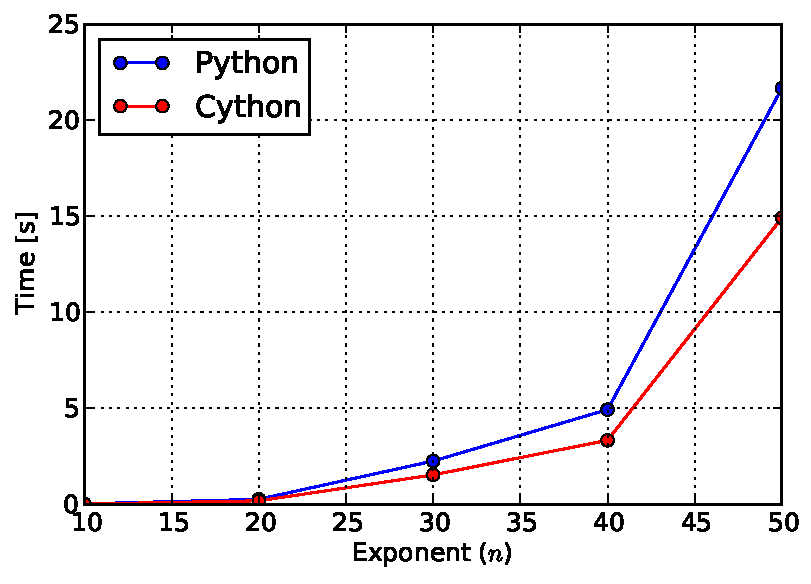
\includegraphics{cython-power.pdf}
\caption{Benchmark: exponentiation of \emph{(27 x + y\textasciicircum{}2 - 15 z)\textasciicircum{}n:math:}.\label{fig-cython-power}}\end{figure}
\begin{figure}[htbp]
\centering

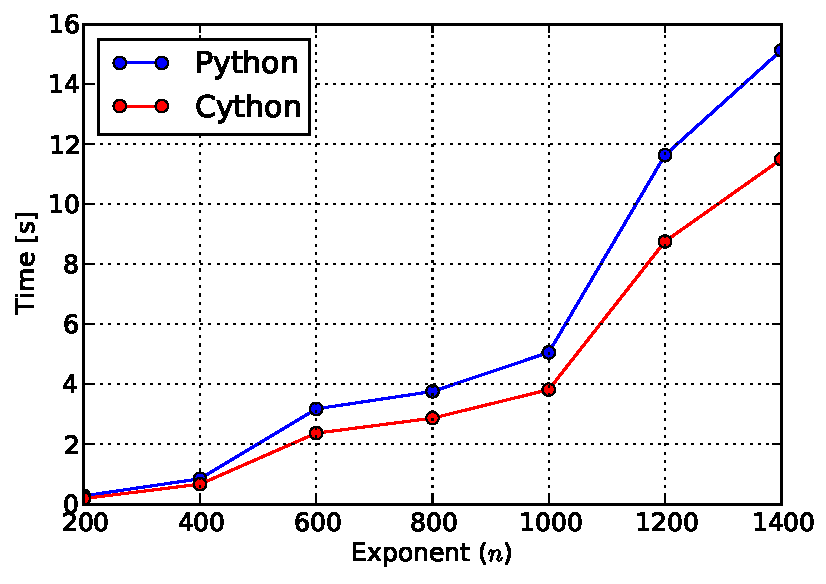
\includegraphics{cython-factor.pdf}
\caption{Benchmark: factorization of {\color{red}\bfseries{}{}`}x\textasciicircum{}n - 1\$ over integers.\label{fig-cython-factor}}{\small }\end{figure}

In future we expect even better improvements when native variables will be used for coefficient
arithmetics. Every algorithm which uses modular approach, which include algorithms for factoring
polynomials, computing GCD or resultants, will benefit from this, because coefficients arising
on the intermediate steps in those algorithms are usually half--words (computations are done in
small finite fields). How to achieve this, without compromising functionality and correctness,
is a subject for future discussion.


\section{Conclusions}



\chapter{Algorithms for algebraic computations}\label{thesis-algorithms}

SymPy implements a wide variety of algorithms for polynomials manipulation, which ranges from
relatively simple algorithms for doing arithmetics of polynomials, to advanced methods for
factoring polynomials into irreducibles over algebraic number fields or computing Gröbner
bases. In this chapter we will shortly describe most important algorithms of polynomials
manipulation module in SymPy. The descriptions will include a brief note on the purpose and
applications of a particular algorithm. Where possible, we will also discuss computational
complexity of an algorithm and possibility for parallelization.

We will also give references to the most influential literature (papers, books, proceedings, etc.)
about every algorithm that will be described in this study. Besides theses bibliographical items,
during development of polynomials manipulation module, we also used several classical books on the
topic of symbolic and algebraic computing: \cite{Davenport1988systems}, \cite{Geddes1992algorithms},
\cite{Gathen1999modern} and \cite{Grabmeier2003algebra}, to name a few, which are considered to be the
main source of knowledge on algorithms and data structures in this field. We also took advantage
of Donald Knuth's famous books, especially the volume concerning semi--numerical algorithms
\cite{Knuth1985seminumerical}. We also used general books on algorithms and data structures, like
\cite{Cormen2001algorithms}, and mathematical tables, e.g \cite{Abramowitz1964handbook} (which was very
useful when implementing special polynomials, e.g. orthogonal polynomials).


\section{Arithmetics of polynomials}

Arithmetics, i.e. addition, subtraction, multiplication, exponentiation and division, of polynomials
form a basis for all other polynomials manipulation algorithms. In SymPy we currently implement only,
so called, \emph{classical algorithms} for this purpose, i.e. repeated squaring algorithm for exponentiation,
and $O(n^2)$ algorithms for multiplication and division, where $n$ is the maximal number of terms in
the set of input polynomials. Over finite fields we use algorithms of \cite{Monagan1993inplace}, which
slightly improve speed of computations over this very specific domain.

An alternative to classical algorithms are, so called, \emph{fast algorithms}, which are sub--quadratic
time algorithms for doing arithmetics polynomials \cite{Moenck1976practical}, \cite{Bernstein2008fast}. Fast
algorithms are usually limited to specific domains of computation, like integers or rationals. The
family includes Karatsuba's and FFT (Fast Fourier Transform) algorithms. The decision was made to use
classical algorithms at this point, because it is not a trivial task to make fast algorithms really
advantageous, especially for small or ill conditioned polynomials. In future, when the module will
stabilize, we will consider implementing fast algorithms, as a companion to classical algorithms,
and use them where it makes sense.

There are other ideas to improve arithmetics of polynomials, especially over integers and rationals.
An interesting example of such optimisation is algorithm of \cite{Fateman2005encoding}, where polynomials
with integer coefficients are encoded as sufficiently large integers and arithmetics are done using
long integer arithmetics, and later results are converted back to polynomials. This is possible by
using an isomorphism (a reversible transformation) between polynomials and integers. To make this
algorithm efficient, we need a very fast integer arithmetics library, like gmpy, which is not always
available on the system. One has to also be aware of the fact that transformations back and forth
may be very costly, especially for large polynomials.


\section{Evaluation of polynomials}

In SymPy we employ Horner scheme \cite{Geddes1992algorithms} for evaluation of univariate polynomials
over arbitrary domains. The algorithm of Horner was proved to be the optimal method for evaluation
of polynomials, which takes minimum number of additions and multiplications necessary to compute
a result. In the multivariate case, Horner scheme is non--unique, thus there are many different
schemes possible, which lead to different evaluation times. Currently we use a \emph{natural} scheme,
which is a consequence of using by default recursive polynomial representation. In the past we
experimented with greedy algorithms for optimizing multivariate Horner scheme \cite{Ceberio2004greedy},
however, without much success. This was because, although evaluation was considerably faster comparing
to the standard scheme, however optimisation times were often comparable to computation times. In future
we may reconsider using some sort of optimisation of polynomial evaluation algorithm in the multivariate
case.

Horner scheme is a very general algorithm, which is also used in SymPy for computing compositions
and rational transformations of polynomials, and many other, which require some sort of efficient
evaluation of polynomials.


\section{The Greatest Common Divisor}

Another fundamental algorithm of polynomials manipulation is the GCD (Greatest Common Divisor)
algorithm, which allows us to compute common factors of two or more polynomials. This is very
useful on its own and as a component of other algorithms, e.g. square--free decomposition or
simplification of rational expressions.

We implement three algorithms for computing GCDs. The most general algorithm is based on
subresultants (a special case of polynomial remainder sequences) and can be used regardless
of the ground domain and polynomial representation. This is also the slowest algorithm, but
very useful if other algorithms fail or are not applicable. Where possible, we use heuristic
GCD algorithm \cite{Liao1995heuristic}, which transforms a problem of computing GCD of polynomials
to integer GCD problem. Although the algorithm is heuristic, with current parametrization it
never failed in SymPy. Daily practice shows that this approach is superior to the algorithm
based on subresultants, however heuristic GCD is only limited to integers and rationals (by
clearing denominators). It also requires very efficient integer GCD algorithm, so it is
beneficial to use gmpy library for this purpose. We also implement an algorithm that uses
Gröbner bases for computing GCD of multivariate polynomials \cite{Cox1997ideals}. This was
historically the first implementation of multivariate polynomial GCD algorithm in SymPy
(see section \ref{thesis-euclid} for details).

In future we plan to implement EEZ--GCD algorithm of Wang \cite{Wang1980eezgcd}, \cite{Moses1973ezgcd},
which we hope will improve computation of GCDs of sparse multivariate polynomials over integers
and rationals. Implementation of EEZ--GCD algorithm should be rather straightforward, because
we already have EEZ polynomial factorization algorithm implemented, and both algorithms share
a common core (variable--by--variable Hensel lifting algorithm), and they differ mainly in the
initialization phase. Having a fast algorithm for sparse polynomials is very important, because
most polynomials that we encounter in real life problems are sparse.

An alternative would be to implement sparse modular algorithm (SPMOD) of Zippel, which is also
optimized for sparse multivariate case. This algorithm is even more interesting in the light
of recent developments \cite{Monagan2004algebraic}, \cite{Javadi2007spmod}, where the algorithm was
successfully employed over algebraic number and function fields. Although there is a simple
idea standing behind SPMOD, this algorithm is considered, in the literature, to be very hard
to implement, because there are many special cases, which have to properly worked out. Thus,
at least for optimizing GCD computations over integers and rationals, we see EEZ algorithm
more beneficial at the moment.

Some parts of modular algorithms can be relatively easily parallelized on multiple processors,
because it often happens that several computations over a smaller domain have to be performed
to compute the GCD in the original domain. For example this is the case in EEZ--GCD algorithm
where, as one of initialization steps, we need to compute several univariate GCDs to compute
the original multivariate GCD. Those univariate GCDs can be very costly, but we have to do
several such computations (at least three) to guarantee correctness of EEZ algorithm (otherwise
the algorithm may fail and would have to be restarted and another sequence of univariate
polynomial GCDs would have to be computed). Those univariate GCDs can be computed in parallel,
greatly improving speed of multivariate GCD algorithm.


\section{Square--free decomposition}

Given a polynomial $f$, square--free decomposition (factorization) of $f$ gives a list of
polynomials (factors) $f_1$, $f_2$, $\ldots$, $f_n$, such that all pairs of polynomials
$(f_i, f_j)$, for $i \not= j$, are co--prime, and $f = f_1 f_2^2 \ldots f_n^n$. Thus each
$f_i$ has no repeated roots. Note that square--free decomposition does not give a true
factorization into irreducibles, although is a very important step in any factorization
algorithm (which we will describe in the following section).

In SymPy we implement the fast algorithm of Yun \cite{Yun1976squarefree} for computing square--free
decompositions in domains of characteristic zero. The cost of computing square--free decomposition
is equivalent to the computation of the greatest common divisor of $f$ and its derivative. Over
finite fields we currently use less efficient algorithm, due to odd but well known behaviour of
derivatives over domains with finite number of elements, where $f'$ might vanish even if $f$ is
non--constant polynomial (e.g. $f = x^k$ over $\F_k$, for any $k >= 2$), which leads to complications
in the algorithm. In future we should implement Yun's algorithm also in this case as well.


\section{Factorization of polynomials}

Algorithms for computing factorizations of polynomials into irreducibles over various domains
are the landmark of symbolic mathematics. The work in this area started early, in ninetieth
century, and algorithms for factoring of univariate and multivariate polynomials over rationals
were invented by Kronecker. Those algorithms had exponential time complexity and were impractical
for any real--life computations. Kronecker's algorithms were the first polynomial factorization
algorithms that were implemented in SymPy.

Over the years mathematicians tried to invent a more efficient method for factoring large polynomials,
focusing their research on univariate polynomials with integer coefficients. A partial breakthrough
came with Hensel's lemma (Hensel lifting algorithm), which allowed to perform computations with integer
valued polynomials over finite fields. Thus, an integer polynomial problem can be transformed into
finite field polynomial problem, then computations can be done in a much smaller (finite) domain and
results can be transformed (lifted) back to the integer polynomial domain.

In 1967, Berlekamp gave first complete factorization algorithm over finite fields. Moreover, this
algorithm had polynomial time complexity. Soon after, Zassenhaus combined Berlekamp's algorithm and
Hensel's lemma, giving first efficient algorithm for polynomial factorization over integers. Although,
the algorithm of Zassenhaus had still exponential time worst--case complexity, on average it behaved
as polynomial time algorithm, allowing to compute with large polynomials with integer coefficients.
This breakthrough stimulated the society and, in the following twenty years after Zassenhaus algorithm
was invented, many other algorithms were invented, covering wider range of coefficient domains and
introducing modular techniques (Hensel's lemma) to the case of multivariate polynomials.


\subsection{Finite fields}

SymPy supports factoring of polynomials over finite fields only in the univariate case (mostly because
originally factoring over finite fields was needed only as a sub--algorithm of polynomial factorization
routines over integers. In future, we may extend support to multivariate case as well, implementing (for
example) algorithm of \cite{Gathen1983polytime}. Over finite fields we have a wide variety of algorithms
implemented. There is Berlekamp's algorithm, which uses linear algebra techniques and is suitable for
factoring over small finite fields. We have also Cantor--Zassenhaus' algorithm, which uses polynomial
algebra and is the default factorization algorithm over this domain, because it performs best for average
inputs. There is also algorithm due to Shoup, Gathen and Kaltofen, which is a sub--quadratic time algorithm,
very efficient for large inputs \cite{Gathen1992frobenious}, \cite{Shoup1993reality}, \cite{Kaltofen1995subquadratic},
\cite{Shoup1995factor} (especially for large finite fields, where the binary logarithm of the size of a
finite field is comparable to the degree of an input polynomial). User can switch between different
algorithms at runtime by setting appropriate options in module's configuration.


\subsection{Integers and rationals}

Factoring algorithms of univariate and multivariate polynomials over integers and rationals are
currently the most important tools among all factorization routines that were implemented in SymPy.

Factorization of polynomials over rationals is done by clearing denominators of coefficients of an input
polynomial and performing factorization over integers. As opposed other algorithms, here the results are
not populated back with the common denominator, but integer coefficients are left in the output, and a
rational common multiplicative coefficient of all factors is left in front of others.

In the univariate case SymPy implements the algorithm of Zassenhaus, which is an exponential time
algorithm, which works by transforming factorization problem over integers to factorization problem
over a small finite field (optimally half--word coefficients, if possible). The resulting factors
are later \emph{lifted} using Hensel's lemma and combined using combinatorial search algorithm to form
\emph{true} univariate factors over integers (also known as searching phase). The last part of this
algorithm makes it exponential time. However, as we previously said, the algorithm behaves as it
had polynomial time complexity, and its true nature is visible only for specially constructed classes
of polynomials (especially those which have very many factors over most or all finite fields). The
unfortunate thing is that polynomials resulting from multivariate or algebraic factoring algorithms
have often exactly those properties. Many heuristics exist to improve the searching phase of Zassenhaus'
algorithm and reduce overall execution time of this method \cite{Abbott2000searching}.

In 1982, a polynomial time algorithm for univariate factoring over integers of Lenstra, Lenstra and
Lovász was invented \cite{Lenstra1982factor}. This was the first polynomial time algorithm for the task.
However, it happens that exponential time algorithms are anyway superior for most inputs and the new
algorithm is only beneficial for very large and very badly conditioned inputs. Thus we did not consider
implementing this algorithm in SymPy. There is, however, an algorithm of van Hoeij \cite{vanHoeij2002knapsack},
which uses a sub--algorithm of LLL, exactly speaking it uses latice basis reduction, to optimize the
searching phase of Zassenhaus algorithm. van Hoeij's algorithm is actually a family of algorithms and
proper parametrisation is significant to make the algorithm very efficient. A parametrisation and some
additional optimisations, which greatly improve van Hoeij's algorithm, can be found in \cite{Belabas2004relative}.
The algorithm has still exponential time complexity, but is superior to any other known algorithm for the
taks of univariate polynomials factorization over integers. We plan to implement this algorithm in near
future in SymPy.

In the multivariate case we implement EEZ algorithm of Wang \cite{Wang1978improved}, which is an improved
version of Musser's algorithm for multivariate polynomial factorization over integers \cite{Musser1975factor},
\cite{Wang1975integers}. The algorithm works by finding a set of valid substitution integers for all but
one variables. This way a univariate polynomial is constructed which is factored and the resulting
factors are used to compute \emph{true} multivariate factors of the input polynomial. Multivariate factors
are constructed using very efficient parallel (variable--by--variable) Hensel lifting algorithm. The
algorithm tries to predict some of the coefficients during each lifting step, reducing significantly
this way execution times. There are other algorithms that could be implemented in SymPy, for example
algorithm of Gao \cite{Gao2003partial}, which factors polynomials via partial differential equations.
However, at this point we do not see a need for implementing another algorithms, because there is
still a lot room for improvements in our implementation of Wang's algorithm.
\subsection{Algebraic number fields}\label{thesis-algebraic}

Currently we use the classical algorithm of Trager \cite{Trager1976algebraic} for computing factorizations
of univariate and multivariate polynomials over algebraic number fields. The algorithm was invented as
a side effect of Trager's work on the task of symbolic integration of rational functions. Trager's
algorithm works by transforming algebraic polynomial factorization problem into integer polynomial
factorization problem, which can lead to very large, ill suited polynomials that are hard to factor
(further optimizations are possible, see \cite{Encarnacion1997norms}). Trager's algorithm support multiple
algebraic extensions by computing a primitive element of all extensions involved. There are other
algorithms, e.g. due to Wang \cite{Wang1976algebraic} or Zhi \cite{Zhi1997optimal}, which can factor with
multiple extensions without computing primitive elements. Benchmarks are, however, not convincing
and it is not clear if those algorithms are really an improvement, comparing to Trager's algorithm
(which is on the other hand much simpler in implementation).


\section{Gröbner bases}

The method of Gröbner bases is a powerful technique for solving problems in commutative
algebra (polynomial ideal theory, algebraic geometry). In chapter \ref{thesis-groebner}
we will describe Gröbner bases in very detail, so we will skip any further discussion
on this topic in this section, to avoid redundancy.


\section{Root isolation}

Polynomials are solvable by radicals only up to degree 4 (inclusive). This is an unfortunate
but well known consequence of Abel--Ruffini theorem. SymPy implements heuristic algorithms
for solving polynomials in terms of radicals in \code{roots()} function. In some cases it is
possible to find roots of higher degree polynomials, by taking advantage of polynomial
factorization and decomposition algorithms, and pattern matching.

This is an obviously limited approach and there is a need, in various areas of symbolic
mathematics, e.g. when solving of systems of polynomial equations \cite{Strzebonski1997computing},
to compute values of roots of a polynomial to a desired precision. This could be done by using
numerical root finding algorithms, like Durand--Kerner's, which has its implementation in mpmath
library and is exposed to the top--level via \code{nroots()} function. However, in pathological
cases, numerical algorithms may fail to compute correct values of polynomials' roots.

To tackle this problem, when the user needs guaranteed error bounds of the computed roots,
symbolic root isolation algorithms should be used. SymPy can isolate roots of polynomials with
rational coefficients over real and complex domains, taking advantage of most recent algorithmic
developments in the field. Symbolic root isolation is not that efficient as numerical root finding,
but it is always successful for arbitrary polynomials, giving, as the result, isolation intervals
of the roots of a polynomial, in the real case, or isolation rectangles, in the complex case.


\subsection{Real roots}

For real root isolation SymPy implements an optimized version \cite{Akritas2008study},
\cite{Akritas2008improving} of continued fractions algorithm \cite{Collins1976descarte}. This
approach allows convergence rate to a solution equivalent to convergence rate of continued
fraction expansion of a real number, giving exact results (points instead of intervals)
whenever possible. For a detailed study of computational complexity of continued fractions
algorithm refer to \cite{Sharma2007complexity}.


\subsection{Complex roots}

Isolation of complex roots is a much more demanding task. In SymPy we implemented the algorithm
of Collins and Krandick \cite{Collins1992infallible}, the best currently known algorithm for symbolic
complex root isolation (it is also implemented in Mathematica, see \cite{MathematicaInternal} for
details).

Collins--Krandick algorithm is an infallible (purely symbolic) algorithm for isolating complex
roots of univariate polynomials with rational and Gaussian rational coefficients. In SymPy we
currently allow only rational coefficients, but extension to the more general domain should be
rather straightforward (Gaussian rational domain has to be implemented).

The algorithm starts with a sufficiently large rectangle, which contains all roots the input
polynomial, it bisects this rectangle, either vertically or horizontally, depending on the
geometry of the isolation rectangle and computes the number of roots in each bisected part.
If there are no roots in a rectangle then such a rectangle is skipped. If there is exactly
one root, then the algorithm returns the rectangle a solution. Otherwise, the new rectangle
is added to a queue and scheduled for further bisection. The initial rectangle is computed
using Cauchy bound, which may give large overestimation on the magnitude of roots. If the
there are no more rectangles left, i.e. each resulting rectangle contains only a single
root (is an isolation rectangle), then the algorithm terminates. After the isolation phase,
resulting rectangles can be further refined to the desired precision.

As only rational coefficients are allowed, this gives the possibility of improving the speed
of computations by isolating strictly complex roots only in the upper half--plane, excluding
the real line (positive imaginary component). Conjugates are located by symmetry and real
roots are located using much more efficient real root isolation algorithm.

An important issue is location of roots on the boundary of an isolation rectangle. The
algorithm can easily count roots in such setup (as opposed to other complex root isolation
algorithm). However, to disambiguate the bisection scheme, where the same could be counted
as a part of two (or more) adjacent rectangles, we only count roots located on the northern
and western edges, and on the north--western corner of an isolation rectangle.

The current implementation of Collins--Krandick algorithm in SymPy is suboptimal and there
are several possible enhancements, some of listed in \cite{Collins1992infallible}, which ought
to make complex root isolation in SymPy much faster.

Collins--Krandick algorithm seems to be a good candidate for parallelization on multiple
processors, although the author is not aware of any work tackling this problem. An approach
would be to schedule refinement of particular isolation rectangles or clusters of rectangles
on different processors. Currently we simply maintain a queue of rectangles in order from
the smallest to the largest and refine each one--by--one on a single CPU.

Previously also we experimented with, so called, global bisection algorithm due to Wilf
\cite{Wilf1978bisection}. As its name suggests, Wilf's algorithm takes advantage of bisection
scheme and operates on rectangles, similarly to Collins--Krandick algorithm, however it uses
Sturm sequences to compute the number of roots in a rectangle and thus is very slow, because
computing polynomial remainder sequences (in particular Sturm sequences) is slow a computationally
demanding process. The other issue is that when a root is located on or even near (there is no
definition of the word \emph{near} in this context) rectangle boundary then the algorithm has to be
restarted with an updated initial configuration. This makes global bisection algorithm fragile
and unpredictable. There are other approaches to symbolic root isolation, see for example
\cite{Pinkert1976complex}.

Collins--Krandick algorithm takes advantage of purely symbolic approach, thus is significantly
slower than rapidly converging numerical algorithms. However, it is possible to turn it into a
mixed symbolic--numerical algorithm, where, in certain conditions, it is possible to replace
symbolic computations with validated numerical computations, without compromising properties
of the original algorithm.

It should be obvious that real root isolation is less computationally intensive than complex
root isolation, so whenever it is known that only real (or even negative or positive) roots
are required, then the domain of computation should be appropriately limited to speed up the
computations (for a detailed discussion see \cite{Collins1996complex}).


\section{Conclusions}

In this chapter we gave a brief description to the most important algorithms of polynomials
manipulation module. There are other algorithms that were implemented in the module, which
also deserve attention and a few words of explanation. Hopefully in some foreseeable future
we will be able to write a more capacious volume, in which we will describe all of them. We
also gave references to the most influential literature that was used to implement those
algorithms or seems promising for further developments in near future. We consider this a
good starting point for people who would be interested in picking up some development tasks
to improve the module.



\chapter{Gröbner bases and their applications}\label{thesis-groebner}

The method of Gröbner bases is a powerful technique for solving problems in commutative
algebra (polynomial ideal theory, algebraic geometry) that was introduced by Bruno Buchberger
in his PhD thesis \cite{Buchberger1965thesis} (for English translation see \cite{Abramson2006translation}
and for a historical background see \cite{Abramson2009history}). Gröbner bases provide a uniform
approach for solving problems that can be expressed in terms of systems of multivariate polynomial
equations. It happens that many practical problems, e.g.  in operational research (graph theory),
can be transformed into sets of polynomials, thus solved using Gröbner bases method.

In this chapter we will give a short theoretical background on Gröbner bases and then we will
show, in a tutorial--like fashion on a series of examples, how to use Gröbner bases machinery
in SymPy. After two very theoretical chapters it is time to show that polynomials manipulation
module, that we wrote for SymPy, is actually useful for solving practical problems. We chose
Gröbner bases for this presentation, because the theory behind Gröbner bases is relatively
simple and there are many non--artificial and non--trivial examples of applications of Gröbner
bases, that can be found in literature, which do not require the reader to have extensive mathematical
knowledge, but also touch many different areas of polynomials manipulation module. However, if some
mathematical background will be needed in a particular example, then we will provide a short introduction
every time additional knowledge is needed.


\section{Short introduction to Gröbner bases}

The Gröbner bases method is a very attractive tool in computer algebra because it is a very
simple to understand and relatively simple to implement (implementation is SymPy consists of less
than 150 lines of code) computational method. The low overhead of the theoretical background of
the principles of the Gröbner bases method (not including the proof of the main theorem, which
is, on the other hand, very complicated) makes is possible to apply Gröbner bases in various
areas of science and engineering, not only by mathematicians.

To introduce the concept of Gröbner bases, following \cite{Buchberger2001systems}, lets consider
a set $F$ of multivariate polynomial equations, i.e. $F = \{ f \in \K\Xn \}$, where $\K$ usually
denotes a field of characteristic zero:
\begin{enumerate}
\item {} 
we transform the set of polynomials $F$ into another set $G$

\item {} 
the obtained set $G$ is called a Gröbner basis of $F$

\item {} 
$G$ has some \emph{nice} properties that the set $F$ does not posses

\item {} 
$F$ and $G$ have exactly the same sets of solutions

\end{enumerate}

The Gröbner bases theory tells us that:
\begin{enumerate}
\item {} 
problems which are difficult to solve in terms of $F$, are \emph{easy} to solve with $G$

\item {} 
there exists an algorithm for transforming arbitrary $F$ into an equivalent set $G$

\end{enumerate}

Taking advantage of this, our approach, in the following sections, will be to understand as much as
possible about $F$ by inspecting the structure and properties of $G$. In some cases we will be given a
set of polynomial equations explicitly. Often, however, our problem will be stated in other \emph{language},
for example in terms of graphs or matrices, and we will need first to transform the original formulation
into a system of polynomials. Then we will be able to reason about the nature of our initial problem by
analyzing the Gröbner basis of the constructed set of polynomial.
\section{Construction of Gröbner bases}\label{gb-construct}

Suppose we are given a finite set of polynomials $F$. The question arises: how to find another set
of polynomials $G$, a Gröbner basis of $F$, such that $F$ and $G$ have the same sets of solutions?
Moreover, is it possible to find $G$ in a systematic (algorithmic) way? If so, does the algorithm
always terminate? These were tough questions as of the first half of the 20th century. However, in
1965 Bruno Buchberger in his PhD thesis gave affirmative answer to all those questions by inventing
an algorithm for constructing Gröbner bases.


\subsection{The notion of s--polynomials}

To introduce the algorithm for computing Gröbner bases, Buchberger defined first the notion of,
so called, s--polynomials. Given two multivariate polynomials $f$ and $g$, suppose that $L$ is the
least common multiple of the leading monomials of $f$ and $g$ with respect to a fixed ordering of
monomials, i.e. $L = \lcm(\LM(f), \LM(g))$, then:
\begin{gather}
\begin{split}\spoly(f, g) = \frac{L}{\LT(f)} f - \frac{L}{\LT(g)} g\end{split}\notag
\end{gather}
where $\LT(\cdot)$ stands for the leading term and $\LM(\cdot)$ stands for the leading monomial of
a polynomial. The definition of s--polynomials can be directly transformed into Python:

\begin{Verbatim}[commandchars=@\[\]]
@PYG[k][def] @PYG[n+nf][s@_polynomial]@PYG[p][(]@PYG[n][f]@PYG[p][,] @PYG[n][g]@PYG[p][)]@PYG[p][:]
    @PYG[k][return] @PYG[n][expand]@PYG[p][(]@PYG[n][lcm]@PYG[p][(]@PYG[n][LM]@PYG[p][(]@PYG[n][f]@PYG[p][)]@PYG[p][,] @PYG[n][LM]@PYG[p][(]@PYG[n][g]@PYG[p][)]@PYG[p][)]@PYG[o][*]@PYG[p][(]@PYG[l+m+mi][1]@PYG[o][/]@PYG[n][LT]@PYG[p][(]@PYG[n][f]@PYG[p][)]@PYG[o][*]@PYG[n][f] @PYG[o][-] @PYG[l+m+mi][1]@PYG[o][/]@PYG[n][LT]@PYG[p][(]@PYG[n][g]@PYG[p][)]@PYG[o][*]@PYG[n][g]@PYG[p][)]@PYG[p][)]
\end{Verbatim}
\noindent
utilizing SymPy`s built--in polynomial manipulation functions \code{LT()}, \code{LM()}, \code{lcm()}
and \code{expand()}, as well as multivariate polynomial arithmetics. For readability purpose, we
skipped in this definition important information about the ordering of polynomials. What is an
ordering of monomials? For now it is sufficient to assume that it exists and is fixed. In the
following sections we will investigate this in detail.


\subsection{What is a Gröbner basis?}

Having the definition of s--polynomials, the fundamental theorem of Gröbner bases (also known as
the Buchberger criterion) is as follows: a set of polynomials $G$ is a Gröbner basis if for all
pairs $(g_i, g_j)$ of polynomials in $G$, the remainder with respect to $G$ of the s--polynomial
of $g_i$ and $g_j$ is zero, i.e.:
\begin{gather}
\begin{split}\forall_{g_i, g_j \in G} \remainder(\spoly(g_i, g_j), G) = 0\end{split}\notag
\end{gather}
(see \cite{Adams1994intro} for details). The theorem is constructive, because the concept of
s--polynomials is well defined and as the remainder procedure we can take the \emph{generalized
division} algorithm (also known as the \emph{normal form} algorithm, see \cite{Cox1997ideals} for a
detailed description). Given a set of polynomials $G$, one can check if $G$ is a Gröbner
basis in a finite number of steps. In SymPy, the generalized division algorithm is implemented
in \code{reduced()} function. As an example, lets consider the following set of polynomials:

\begin{Verbatim}[commandchars=@\[\]]
@PYG[g+gp][@textgreater[]@textgreater[]@textgreater[] ]@PYG[n][F] @PYG[o][=] @PYG[p][@PYGZlb[]]@PYG[n][f1]@PYG[p][,] @PYG[n][f2]@PYG[p][@PYGZrb[]] @PYG[o][=] @PYG[p][@PYGZlb[]]@PYG[n][x]@PYG[o][*]@PYG[n][y] @PYG[o][-] @PYG[l+m+mi][2]@PYG[o][*]@PYG[n][y]@PYG[p][,] @PYG[n][x]@PYG[o][*]@PYG[o][*]@PYG[l+m+mi][2] @PYG[o][-] @PYG[l+m+mi][2]@PYG[o][*]@PYG[n][y]@PYG[o][*]@PYG[o][*]@PYG[l+m+mi][2]@PYG[p][@PYGZrb[]]
\end{Verbatim}
\noindent
There are only two polynomials in $F$ so it is sufficient to check just a single pair to see
if $F$ is a Gröbner basis or not. Lets apply Buchberger criterion to $f_1$ and $f_2$:

\begin{Verbatim}[commandchars=@\[\]]
@PYG[g+gp][@textgreater[]@textgreater[]@textgreater[] ]@PYG[n][s@_polynomial]@PYG[p][(]@PYG[n][f1]@PYG[p][,] @PYG[n][f2]@PYG[p][)]
@PYG[g+go][            3]
@PYG[g+go][-2*x*y + 2*y]

@PYG[g+gp][@textgreater[]@textgreater[]@textgreater[] ]@PYG[n][reduced]@PYG[p][(]@PYG[n][@_]@PYG[p][,] @PYG[n][F]@PYG[p][)]@PYG[p][@PYGZlb[]]@PYG[l+m+mi][1]@PYG[p][@PYGZrb[]]
@PYG[g+go][   3]
@PYG[g+go][2*y  - 4*y]
\end{Verbatim}
\noindent
We computed the s--polynomial of $f_1$ and $f_2$ and the resulting remainder is non--zero, so
$F$ isn't a Gröbner basis. Lets see what will happen when we adjoin this remainder to $F$:

\begin{Verbatim}[commandchars=@\[\]]
@PYG[g+gp][@textgreater[]@textgreater[]@textgreater[] ]@PYG[n][f3] @PYG[o][=] @PYG[n][@_]
@PYG[g+gp][@textgreater[]@textgreater[]@textgreater[] ]@PYG[n][F]@PYG[o][.]@PYG[n][append]@PYG[p][(]@PYG[n][f3]@PYG[p][)]
\end{Verbatim}
\noindent
Now we have three polynomials in $F$ and three pairs to check, i.e. $(f_1, f_2)$, $(f_1, f_3)$
and $(f_2, f_3)$ (actually only the two new pairs, but lets check all three for completeness):

\begin{Verbatim}[commandchars=@\[\]]
@PYG[g+gp][@textgreater[]@textgreater[]@textgreater[] ]@PYG[n][s@_polynomial]@PYG[p][(]@PYG[n][f1]@PYG[p][,] @PYG[n][f2]@PYG[p][)]
@PYG[g+go][            3]
@PYG[g+go][-2*x*y + 2*y]

@PYG[g+gp][@textgreater[]@textgreater[]@textgreater[] ]@PYG[n][reduced]@PYG[p][(]@PYG[n][@_]@PYG[p][,] @PYG[n][F]@PYG[p][)]@PYG[p][@PYGZlb[]]@PYG[l+m+mi][1]@PYG[p][@PYGZrb[]]
@PYG[g+go][0]

@PYG[g+gp][@textgreater[]@textgreater[]@textgreater[] ]@PYG[n][s@_polynomial]@PYG[p][(]@PYG[n][f1]@PYG[p][,] @PYG[n][f3]@PYG[p][)]
@PYG[g+go][           3]
@PYG[g+go][2*x*y - 2*y]

@PYG[g+gp][@textgreater[]@textgreater[]@textgreater[] ]@PYG[n][reduced]@PYG[p][(]@PYG[n][@_]@PYG[p][,] @PYG[n][F]@PYG[p][)]@PYG[p][@PYGZlb[]]@PYG[l+m+mi][1]@PYG[p][@PYGZrb[]]
@PYG[g+go][0]

@PYG[g+gp][@textgreater[]@textgreater[]@textgreater[] ]@PYG[n][s@_polynomial]@PYG[p][(]@PYG[n][f2]@PYG[p][,] @PYG[n][f3]@PYG[p][)]
@PYG[g+go][     2      5]
@PYG[g+go][2*y*x  - 2*y]

@PYG[g+gp][@textgreater[]@textgreater[]@textgreater[] ]@PYG[n][reduced]@PYG[p][(]@PYG[n][@_]@PYG[p][,] @PYG[n][F]@PYG[p][)]@PYG[p][@PYGZlb[]]@PYG[l+m+mi][1]@PYG[p][@PYGZrb[]]
@PYG[g+go][0]
\end{Verbatim}
\noindent
All reductions resulted in zero reminders, so the extended $F$ is a Gröbner basis. This simple
observation leads to an algorithmic procedure for computing Gröbner bases, which we will fully
describe in \ref{gb-toy}.


\subsection{Reduced Gröbner bases}

The definition of the concept of Gröbner bases, we gave so far, has one serious flaw. Suppose we
are given two structurally distinct systems of polynomials $F$ and $F'$. We would like to know if
those systems are equivalent. We can compute Gröbner bases $G$ and $G'$ of $F$ and $F'$ respectively.
With the current definition of Gröbner bases we can't tell anything about the relation between $F$
and $F'$ by looking at $G$ and $G'$. However, the Gröbner bases theory tells us that when we compute
reduced Gröbner bases of those two systems of polynomials, then $F$ is equivalent to $F'$ if the reduced
Gröbner bases are equal, i.e. $G = G'$. This is a very strong and important result, because it allows
us to reason about systems of polynomial by looking only at their reduced Gröbner bases.

Lets now provide the definition of the concept of reduced Gröbner bases. We will reuse the generalized
division algorithm for this purpose. Given a set of polynomials $G$, which is a Gröbner basis by the
Buchberger criterion, then $G$ is a reduced Gröbner basis when the following statement holds:
\begin{gather}
\begin{split}\forall_{g \in G} \remainder(g, G - \{g\}) = g \wedge g\;\mbox{is monic}\end{split}\notag
\end{gather}
Following this definition, given a Gröbner basis $G$, one can compute a reduced version of $G$
simply by reducing each element $g \in G$ with respect to all other elements of the basis and, in
the end, making all polynomials in $G$ monic. In the remainder of this chapter we will focus only
on reduced Gröbner bases.
\subsection{Toy Buchberger algorithm}\label{gb-toy}

We are ready to describe the Buchberger algorithm. The algorithm proceeds as follows: take a
set of polynomials $F$ and set initially $G := F$, where $G$ will be the desired Gröbner
basis of $F$ at the and of this procedure. Next apply the Buchberger criterion to see if
$G$ is already a Gröbner basis. If this is the case, reduce each polynomial in $G$ with
respect to other polynomials in $G$ and stop. Otherwise pick a pair of polynomials $f_1$ and
$f_2$ from $G$, and compute their s--polynomial. If the remainder with respect to $G$ of the
s--polynomial is non--zero, then adjoin it to $G$. Iterate until $G$ is a Gröbner basis.

This simple procedure can be easily coded in Python in just a couple of minutes using previously
defined \code{s\_polynomial()} and SymPy`s built--in \code{reduced()} functions:

\begin{Verbatim}[commandchars=@\[\]]
@PYG[k][def] @PYG[n+nf][buchberger]@PYG[p][(]@PYG[n][F]@PYG[p][,] @PYG[n][reduced]@PYG[o][=]@PYG[n+nb+bp][True]@PYG[p][)]@PYG[p][:]
    @PYG[l+s+sd]["""Toy implementation of Buchberger algorithm. """]
    @PYG[n][G]@PYG[p][,] @PYG[n][pairs] @PYG[o][=] @PYG[n+nb][list]@PYG[p][(]@PYG[n][F]@PYG[p][)]@PYG[p][,] @PYG[n+nb][set]@PYG[p][(]@PYG[p][@PYGZlb[]]@PYG[p][@PYGZrb[]]@PYG[p][)]

    @PYG[k][for] @PYG[n][i]@PYG[p][,] @PYG[n][f1] @PYG[o+ow][in] @PYG[n+nb][enumerate]@PYG[p][(]@PYG[n][F]@PYG[p][)]@PYG[p][:]
        @PYG[k][for] @PYG[n][f2] @PYG[o+ow][in] @PYG[n][F]@PYG[p][@PYGZlb[]]@PYG[n][i]@PYG[o][+]@PYG[l+m+mi][1]@PYG[p][:]@PYG[p][@PYGZrb[]]@PYG[p][:]
            @PYG[n][pairs]@PYG[o][.]@PYG[n][add]@PYG[p][(]@PYG[p][(]@PYG[n][f1]@PYG[p][,] @PYG[n][f2]@PYG[p][)]@PYG[p][)]

    @PYG[k][while] @PYG[n][pairs]@PYG[p][:]
        @PYG[n][f1]@PYG[p][,] @PYG[n][f2] @PYG[o][=] @PYG[n][pairs]@PYG[o][.]@PYG[n][popitem]@PYG[p][(]@PYG[p][)]

        @PYG[n][s] @PYG[o][=] @PYG[n][s@_polynomial]@PYG[p][(]@PYG[n][f1]@PYG[p][,] @PYG[n][f2]@PYG[p][)]
        @PYG[n][@_]@PYG[p][,] @PYG[n][h] @PYG[o][=] @PYG[n][reduced]@PYG[p][(]@PYG[n][s]@PYG[p][,] @PYG[n][G]@PYG[p][)]

        @PYG[k][if] @PYG[n][h] @PYG[o][!=] @PYG[l+m+mi][0]@PYG[p][:]
            @PYG[k][for] @PYG[n][g] @PYG[o+ow][in] @PYG[n][G]@PYG[p][:]
                @PYG[n][pairs]@PYG[o][.]@PYG[n][add]@PYG[p][(]@PYG[p][(]@PYG[n][g]@PYG[p][,] @PYG[n][h]@PYG[p][)]@PYG[p][)]

            @PYG[n][G]@PYG[o][.]@PYG[n][append]@PYG[p][(]@PYG[n][g]@PYG[p][)]

    @PYG[k][if] @PYG[n][reduced]@PYG[p][:]
        @PYG[k][for] @PYG[n][i]@PYG[p][,] @PYG[n][g] @PYG[o+ow][in] @PYG[n+nb][enumerate]@PYG[p][(]@PYG[n][G]@PYG[p][)]@PYG[p][:]
            @PYG[n][@_]@PYG[p][,] @PYG[n][G]@PYG[p][@PYGZlb[]]@PYG[n][i]@PYG[p][@PYGZrb[]] @PYG[o][=] @PYG[n][reduced]@PYG[p][(]@PYG[n][g]@PYG[p][,] @PYG[n][G]@PYG[p][@PYGZlb[]]@PYG[p][:]@PYG[n][i]@PYG[p][@PYGZrb[]] @PYG[o][+] @PYG[n][G]@PYG[p][@PYGZlb[]]@PYG[n][i]@PYG[o][+]@PYG[l+m+mi][1]@PYG[p][:]@PYG[p][@PYGZrb[]]@PYG[p][)]

        @PYG[n][G] @PYG[o][=] @PYG[n+nb][map]@PYG[p][(]@PYG[n][monic]@PYG[p][,] @PYG[n][G]@PYG[p][)]

    @PYG[k][return] @PYG[n][G]
\end{Verbatim}
\noindent
Lets analyze \code{buchberger()} step--by--step. As the first step we assign $G$ with the input
system of polynomial equations $F$ and generate a set with all (unordered) pairs of polynomials
from $F$. We will use this set to verify the Buchberger criterion for $G$. Next we enter a loop,
which will execute until there are \emph{critical} pairs to check. If there are no more pairs, then
the Buchberger criterion is satisfied and $G$ is a Gröbner basis. In the loop, we take a pair
of polynomials $f_1$ and $f_2$, and compute their s--polynomial and its reduction with respect
to the current basis. If the reduction is non--zero, we adjoin new element to $G$ and update
the set of \emph{critical} pairs. When the loop terminates we obtain a Gröbner basis of $F$. In
the final step of the algorithm, if \code{reduced} flag is set, we reduce each element of the basis
with respect to other elements and make each element monic, obtaining a reduced Gröbner basis.

As it was done with the definition of the function for computing s--polynomials, also in this case
we simplified the implementation by skipping additional information about the ordering of monomials.
This is not an issue, because SymPy assumes \emph{lexicographic} ordering by default and allows to use
\emph{context managers} for configuring ordering post facto.


\subsection{Termination of the algorithm}

Although the Buchberger algorithm is very simple, its termination isn't trivial. At the startup
of this procedure there is only a finite number of pairs of polynomials for which the corresponding
s--polynomials have to be computed. Some of those pairs lead to non--zero reductions, hence $G$ is
growing and the number of additional pairs, that have to be taken into consideration, also grows.
Buchberger proved that this process ends in a finite number of steps. Thus we are guaranteed that
for arbitrary set of polynomials we can compute a corresponding Gröbner basis in finite time.
An interesting question arises: how much time is actually needed to compute such a basis? We will
postpone answer to this question till the end of chapter, where we will discuss complexity of the
Buchberger algorithm and efficiency of SymPy`s Gröbner bases implementation.


\section{Computing Gröbner bases with SymPy}

Although the toy implementation of the Buchberger algorithm, presented in the previous section, can
be used for experimenting with Gröbner bases, its implementation is too naive to make it useful
for solving more complicated problems. For the purpose of computing reduced Gröbner bases with
respect to various orderings of monomials, SymPy has a built--in function \code{groebner()}, which
implements a much more efficient version of Buchberger algorithm.

The main difference between those two implementations is that \code{groebner()} uses several criteria
for cutting down the number of polynomial divisions (actually reductions by a set of polynomials), which
are the central and most expensive part of the Buchberger algorithm. There wouldn't be nothing special
about this, however, most divisions give zero remainder as the result and do not lead to change of
a Gröbner basis. This way most divisions are just \emph{useless} and an efficient implementation of the
Buchberger algorithm must accommodate for this, avoiding as many of those useless divisions as possible.

Several criteria were invented by the author of the Gröbner bases method a few years after the
algorithm was introduced. Later on, other more powerful elimination criteria were developed, for
example, heuristic criteria for lexicographic ordering of monomials \cite{Czapor1991heuristic} or, so
called, \emph{sugar flavour} (see \cite{Giovini1991sugar} for details).
\section{Admissible orderings of monomials}\label{thesis-orderings}

The main reason for our interest in Gröbner bases is that they have \emph{nicer} properties, compared
to other systems of polynomials. Depending on what properties we actually need, we can compute a
Gröbner basis of a given system with respect to a specific ordering of monomials. The choice of
monomial order is significant, because different orderings will lead to different properties of the
resulting basis. Moreover, for a particular system of polynomials, one ordering will make computations
feasible, whereas another will make Buchberger algorithm executing for ages. In the following sections
we will give examples showing why the right choice of monomial order is so important.

There are currently three admissible orderings of monomials implemented in SymPy:
\begin{quote}
\begin{description}
\item[\textbf{lex}] \leavevmode
pure lexicographic order

\item[\textbf{grlex}] \leavevmode
total degree order with ties broken by lexicographic order

\item[\textbf{grevlex}] \leavevmode
total degree order with ties broken by reversed lexicographic order

\end{description}
\end{quote}

Ordering of monomials can be given to \code{groebner()} using \code{order} keyword argument. The default
is \code{lex} order, as it is the most frequently used monomial order, because it leads to, so called,
\emph{elimination} property. The specification of the required ordering of monomials can be passed as a
string via \code{order} keyword or as a single argument function. The other option gives the possibility
of inventing our own orderings of monomials. In this case, however, SymPy won't check if the given
function defines an admissible ordering or not.

Suppose we have a system of two bivariate polynomials \code{f1, f2 = {[}2*x**2*y + x*y**4, x**2 + y + 1{]}}.
We can inspect the leading terms with respect two different orderings of monomials of a polynomial with
assistance of \code{LT()} function:

\begin{Verbatim}[commandchars=@\[\]]
@PYG[g+gp][@textgreater[]@textgreater[]@textgreater[] ]@PYG[n][LT]@PYG[p][(]@PYG[n][f1]@PYG[p][,] @PYG[n][x]@PYG[p][,] @PYG[n][y]@PYG[p][,] @PYG[n][order]@PYG[o][=]@PYG[l+s][']@PYG[l+s][lex]@PYG[l+s][']@PYG[p][)]
@PYG[g+go][   2]
@PYG[g+go][2*x *y]

@PYG[g+gp][@textgreater[]@textgreater[]@textgreater[] ]@PYG[n][LT]@PYG[p][(]@PYG[n][f1]@PYG[p][,] @PYG[n][x]@PYG[p][,] @PYG[n][y]@PYG[p][,] @PYG[n][order]@PYG[o][=]@PYG[l+s][']@PYG[l+s][grlex]@PYG[l+s][']@PYG[p][)]
@PYG[g+go][   4]
@PYG[g+go][x*y]
\end{Verbatim}
\noindent
Similarly as in \code{groebner()} function, \code{LT()} assumes \emph{lexicographic} ordering  of monomials by
default. We observe, in the above example, that \code{LT()} picks up different terms depending on the
chosen ordering. This happens, because in the case of \code{grlex} ordering the total degree of a monomial
is more important than the sequence exponents of that monomial. Differences between leading terms computed
by \code{LT()} influence computations of Gröbner bases:

\begin{Verbatim}[commandchars=@\[\]]
@PYG[g+gp][@textgreater[]@textgreater[]@textgreater[] ]@PYG[n][groebner]@PYG[p][(]@PYG[p][@PYGZlb[]]@PYG[n][f1]@PYG[p][,] @PYG[n][f2]@PYG[p][@PYGZrb[]]@PYG[p][,] @PYG[n][x]@PYG[p][,] @PYG[n][y]@PYG[p][,] @PYG[n][order]@PYG[o][=]@PYG[l+s][']@PYG[l+s][lex]@PYG[l+s][']@PYG[p][)]
@PYG[g+go][[                   7    4                                          ]]
@PYG[g+go][[ 2                y    y       2         8    7      3      2      ]]
@PYG[g+go][[x  + y + 1, x*y + -- + -- + 2*y  + 2*y, y  + y  + 4*y  + 8*y  + 4*y]]
@PYG[g+go][[                  2    2                                           ]]

@PYG[g+gp][@textgreater[]@textgreater[]@textgreater[] ]@PYG[n][groebner]@PYG[p][(]@PYG[p][@PYGZlb[]]@PYG[n][f1]@PYG[p][,] @PYG[n][f2]@PYG[p][@PYGZrb[]]@PYG[p][,] @PYG[n][x]@PYG[p][,] @PYG[n][y]@PYG[p][,] @PYG[n][order]@PYG[o][=]@PYG[l+s][']@PYG[l+s][grlex]@PYG[l+s][']@PYG[p][)]
@PYG[g+go][[   4      2             2            5    4   2        ]]
@PYG[g+go][[x*y  - 2*y  - 2*y, 2*x*y  + 2*x*y + y  + y , x  + y + 1]]
\end{Verbatim}
\noindent
Originally orderings of monomials were implemented as comparison functions and passed to \href{http://docs.python.org/library/functions.html\#sorted}{\code{sorted()}}
built--in function via \code{cmp} keyword argument. This approach was inefficient, because the nature of
the sorting algorithm required to compute ordering information (e.g. total degree) about a particular
monomial multiple times in this scheme. Eventually, \code{cmp}--style sorting was dropped in Python 3.0,
in favour of \code{key}--based sorting \cite{PythonIssue1771}. The new implementation of orderings of monomials
is based on the concept of \code{key}--functions. When implementing user defined orderings, one must conform
to the new approach.

In principle, in the \code{key}--based approach, one has to return all required ordering information about
a particular monomial in a form of tuple (with correct order of elements). In the case of \emph{lexicographic
ordering} of monomials, this information simply consists of the input monomial itself:

\begin{Verbatim}[commandchars=@\[\]]
@PYG[k][def] @PYG[n+nf][monomial@_lex@_key]@PYG[p][(]@PYG[n][monom]@PYG[p][)]@PYG[p][:]
    @PYG[l+s+sd]["""Key function for sorting monomials in lexicographic order. """]
    @PYG[k][return] @PYG[n][monom]
\end{Verbatim}
\noindent
The above is an exact excerpt from \code{sympy/polys/monomialtools.py}, where orderings of monomials are
implemented. In the case of \emph{graded lexicographic ordering} we have an additional information, which is
the total degree of an input monomial, so the key function for \code{grlex} order is defined as follows:

\begin{Verbatim}[commandchars=@\[\]]
@PYG[k][def] @PYG[n+nf][monomial@_grlex@_key]@PYG[p][(]@PYG[n][monom]@PYG[p][)]@PYG[p][:]
    @PYG[l+s+sd]["""Key function for sorting monomials in graded lexicographic order. """]
    @PYG[k][return] @PYG[p][(]@PYG[n+nb][sum]@PYG[p][(]@PYG[n][monom]@PYG[p][)]@PYG[p][,] @PYG[n][monom]@PYG[p][)]
\end{Verbatim}
\noindent
This approach generalizes to other orderings as well. One should also note that the order variables is
also an important factor when computing Gröbner bases, as there are $n!$ specific orderings for a
given ordering of monomials (where $n$ is the number of variables involved in computations).


\section{Specialization of Gröbner bases}

The Gröbner bases algorithm specializes to:
\begin{enumerate}
\item {} 
\emph{Gauss' algorithm} for linear polynomials

\item {} 
\emph{Euclid's algorithm} for univariate polynomials

\end{enumerate}


\subsection{Special case 1: Gauss' algorithm}

Lets consider the following system of linear equations:
\begin{gather}
\begin{split}\left\{
\begin{array}{rcl}
   x + 5 y &=& 2    \\
-3 x + 6 y &=& 15
\end{array}
\right.\end{split}\notag
\end{gather}
which can be written in Python as:

\begin{Verbatim}[commandchars=@\[\]]
@PYG[g+gp][@textgreater[]@textgreater[]@textgreater[] ]@PYG[n][F] @PYG[o][=] @PYG[p][@PYGZlb[]]@PYG[n][x] @PYG[o][+] @PYG[l+m+mi][5]@PYG[o][*]@PYG[n][y] @PYG[o][-] @PYG[l+m+mi][2]@PYG[p][,] @PYG[o][-]@PYG[l+m+mi][3]@PYG[o][*]@PYG[n][x] @PYG[o][+] @PYG[l+m+mi][6]@PYG[o][*]@PYG[n][y] @PYG[o][-] @PYG[l+m+mi][15]@PYG[p][@PYGZrb[]]
\end{Verbatim}
\noindent
It's a simple system, so it can be solved by hand. We can, however, use Gröbner bases
machinery to solve this system algorithmically:

\begin{Verbatim}[commandchars=@\[\]]
@PYG[g+gp][@textgreater[]@textgreater[]@textgreater[] ]@PYG[n][groebner]@PYG[p][(]@PYG[n][F]@PYG[p][,] @PYG[n][x]@PYG[p][,] @PYG[n][y]@PYG[p][)]
@PYG[g+go][@PYGZlb[]x + 3, y - 1@PYGZrb[]]
\end{Verbatim}
\noindent
As the result we got a list of two polynomials. From te list we can obtain the solution
of the system, which is $x = -3$ and $y = 1$ in this case. The same can be computed using
a much more traditional tool in the field of linear algebra, mainly using Gauss--Jordan
algorithm:

\begin{Verbatim}[commandchars=@\[\]]
@PYG[g+gp][@textgreater[]@textgreater[]@textgreater[] ]@PYG[n][solve]@PYG[p][(]@PYG[n][F]@PYG[p][,] @PYG[n][x]@PYG[p][,] @PYG[n][y]@PYG[p][)]
@PYG[g+go][{x: -3, y: 1}]
\end{Verbatim}
\noindent
We obtained the same solution but in the dictionary form this time. It's interesting to
notice that currently, at least for small inputs, the Gröbner bases approach is much
efficient than a specialized solver. Lets compare those two methods:

\begin{Verbatim}[commandchars=@\[\]]
@PYG[g+gp][@textgreater[]@textgreater[]@textgreater[] ]@PYG[o][@%]@PYG[n][timeit] @PYG[n][groebner]@PYG[p][(]@PYG[n][F]@PYG[p][,] @PYG[n][x]@PYG[p][,] @PYG[n][y]@PYG[p][)]
@PYG[g+go][100 loops, best of 3: 5.15 ms per loop]

@PYG[g+gp][@textgreater[]@textgreater[]@textgreater[] ]@PYG[o][@%]@PYG[n][timeit] @PYG[n][solve]@PYG[p][(]@PYG[n][F]@PYG[p][,] @PYG[n][x]@PYG[p][,] @PYG[n][y]@PYG[p][)]
@PYG[g+go][10 loops, best of 3: 22.7 ms per loop]
\end{Verbatim}
\noindent
An explanation of this result is as follows: Gröbner bases utilize very efficient core
of polynomials manipulation module, whereas \code{solve()} uses inefficient implementation
of linear algebra in SymPy. This situation will change and the observed phenomenon will
disappear in near future, when linear algebra module will be refactored (using similar
approach to what was done with polynomials manipulation module).
\subsection{Special case 2: Euclid's algorithm}\label{thesis-euclid}

Lets now focus on the other case, i.e. on computation of greatest common divisors of polynomials.
For this, consider two univariate polynomials \code{f} and \code{g}, both in the indeterminate \code{x},
with coefficients in the ring of integers:

\begin{Verbatim}[commandchars=@\[\]]
@PYG[g+gp][@textgreater[]@textgreater[]@textgreater[] ]@PYG[n][f] @PYG[o][=] @PYG[n][expand]@PYG[p][(]@PYG[p][(]@PYG[n][x] @PYG[o][-] @PYG[l+m+mi][2]@PYG[p][)]@PYG[o][*]@PYG[o][*]@PYG[l+m+mi][3] @PYG[o][*] @PYG[p][(]@PYG[n][x] @PYG[o][+] @PYG[l+m+mi][3]@PYG[p][)]@PYG[o][*]@PYG[o][*]@PYG[l+m+mi][4] @PYG[o][*] @PYG[p][(]@PYG[n][x] @PYG[o][+] @PYG[l+m+mi][7]@PYG[p][)]@PYG[p][)]
@PYG[g+gp][@textgreater[]@textgreater[]@textgreater[] ]@PYG[n][g] @PYG[o][=] @PYG[n][expand]@PYG[p][(]@PYG[p][(]@PYG[n][x] @PYG[o][+] @PYG[l+m+mi][2]@PYG[p][)]@PYG[o][*]@PYG[o][*]@PYG[l+m+mi][3] @PYG[o][*] @PYG[p][(]@PYG[n][x] @PYG[o][+] @PYG[l+m+mi][3]@PYG[p][)]@PYG[o][*]@PYG[o][*]@PYG[l+m+mi][3] @PYG[o][*] @PYG[p][(]@PYG[n][x] @PYG[o][+] @PYG[l+m+mi][7]@PYG[p][)]@PYG[p][)]
\end{Verbatim}
\noindent
We can easily see that those polynomials have to factors in common (of multiplicity three
and one respectively). Lets verify this observation using Gröbner bases algorithm:

\begin{Verbatim}[commandchars=@\[\]]
@PYG[g+gp][@textgreater[]@textgreater[]@textgreater[] ]@PYG[n][groebner]@PYG[p][(]@PYG[p][@PYGZlb[]]@PYG[n][f]@PYG[p][,] @PYG[n][g]@PYG[p][@PYGZrb[]]@PYG[p][)]
@PYG[g+go][[ 4       3       2              ]]
@PYG[g+go][[x  + 16*x  + 90*x  + 216*x + 189]]
\end{Verbatim}
\noindent
We obtained a polynomial of degree four which clearly verifies observation concerning
multiplicities of the commons factors of \code{f} and \code{g}. Lets add more structure to
the computed polynomial GCD using factorization:

\begin{Verbatim}[commandchars=@\[\]]
@PYG[g+gp][@textgreater[]@textgreater[]@textgreater[] ]@PYG[n][factor]@PYG[p][(]@PYG[n][@_]@PYG[p][@PYGZlb[]]@PYG[l+m+mi][0]@PYG[p][@PYGZrb[]]@PYG[p][)]
@PYG[g+go][       3]
@PYG[g+go][(x + 3) *(x + 7)]
\end{Verbatim}
\noindent
Now we can clearly see the common factors of the input polynomials. Although utilization of
Gröbner bases algorithm for computing GCDs of univariate polynomials is very fancy, there
are much more efficient algorithms for this purpose. In SymPy we currently use heuristic GCD
algorithm over integers and rationals, and subresultants over other domains.

Moreover, Gröbner bases can be used to compute greatest common divisors of multivariate
polynomials \cite{Cox1997ideals}. The algorithm reduces the problem of finding the GCD of two
multivariate polynomials, say \code{f} and \code{g}, into the problem of finding their least
common multiple. The final result is obtained using the well known formula that relates
GCD with LCM:
\hypertarget{equation-gcdlcm}{}\begin{gather}
\begin{split}\gcd(f, g) = \frac{f \cdot g}{\lcm(f, g)}\end{split}\label{src/groebner-gcdlcm}
\end{gather}
The multivariate polynomial LCM is computed as the unique generator of the intersection of
the two ideals generated by \code{f} and \code{g}. The approach is to compute a Gröbner basis
of $t \cdot f$ and $(1 - t) \cdot g$, where $t$ is an unrelated variable, with respect to
lexicographic order of terms which eliminates $t$. The polynomial LCM of \code{f} and \code{g}
is the last element of the computed Gröbner basis.

As an example consider the following two bivariate polynomials over integers:

\begin{Verbatim}[commandchars=@\[\]]
@PYG[g+gp][@textgreater[]@textgreater[]@textgreater[] ]@PYG[n][f] @PYG[o][=] @PYG[n][expand]@PYG[p][(]@PYG[p][(]@PYG[n][x] @PYG[o][-] @PYG[l+m+mi][1]@PYG[p][)]@PYG[o][*]@PYG[o][*]@PYG[l+m+mi][3] @PYG[o][*] @PYG[p][(]@PYG[n][x] @PYG[o][+] @PYG[n][y]@PYG[p][)]@PYG[o][*]@PYG[o][*]@PYG[l+m+mi][4] @PYG[o][*] @PYG[p][(]@PYG[n][x] @PYG[o][-] @PYG[n][y]@PYG[p][)]@PYG[p][)]
@PYG[g+gp][@textgreater[]@textgreater[]@textgreater[] ]@PYG[n][g] @PYG[o][=] @PYG[n][expand]@PYG[p][(]@PYG[p][(]@PYG[n][x] @PYG[o][+] @PYG[l+m+mi][1]@PYG[p][)]@PYG[o][*]@PYG[o][*]@PYG[l+m+mi][3] @PYG[o][*] @PYG[p][(]@PYG[n][x] @PYG[o][+] @PYG[n][y]@PYG[p][)]@PYG[o][*]@PYG[o][*]@PYG[l+m+mi][3] @PYG[o][*] @PYG[p][(]@PYG[n][x] @PYG[o][-] @PYG[n][y]@PYG[p][)]@PYG[p][)]
\end{Verbatim}
\noindent
To compute the GCD of \code{f} and \code{g} we will introduce new variable $t$ and then we will
find a Gröbner basis of $t \cdot f$ and $(1 - t) \cdot g$ which eliminates $t$:

\begin{Verbatim}[commandchars=@\[\]]
@PYG[g+gp][@textgreater[]@textgreater[]@textgreater[] ]@PYG[n][basis] @PYG[o][=] @PYG[n][groebner]@PYG[p][(]@PYG[p][@PYGZlb[]]@PYG[n][t]@PYG[o][*]@PYG[n][f]@PYG[p][,] @PYG[p][(]@PYG[l+m+mi][1] @PYG[o][-] @PYG[n][t]@PYG[p][)]@PYG[o][*]@PYG[n][g]@PYG[p][@PYGZrb[]]@PYG[p][,] @PYG[n][t]@PYG[p][,] @PYG[n][x]@PYG[p][,] @PYG[n][y]@PYG[p][)]
\end{Verbatim}
\noindent
Note that the order of variables is significant. We chose $t$ to be of higher rank than
$x$ or $y$ to allow Gröbner basis algorithm to eliminate it from the last element of
the basis. As the relative rank of $x$ and $y$ is not important in this case, we can
rewrite the above expression in a slightly different form:

\begin{Verbatim}[commandchars=@\[\]]
@PYG[g+gp][@textgreater[]@textgreater[]@textgreater[] ]@PYG[n][basis] @PYG[o][=] @PYG[n][groebner]@PYG[p][(]@PYG[p][@PYGZlb[]]@PYG[n][t]@PYG[o][*]@PYG[n][f]@PYG[p][,] @PYG[p][(]@PYG[l+m+mi][1] @PYG[o][-] @PYG[n][t]@PYG[p][)]@PYG[o][*]@PYG[n][g]@PYG[p][@PYGZrb[]]@PYG[p][,] @PYG[n][wrt]@PYG[o][=]@PYG[n][t]@PYG[p][)]
\end{Verbatim}
\noindent
This syntax signifies that the only important knowledge here is that $t$ comes before
any other variable. This approach is also far more general because we could use input
polynomials with more variables without changing the algorithm, as long as there is no
clash of variables with $t$. We can guarantee that this won't happen by declaring $t$
as a \emph{dummy} variable, i.e. \code{t = Symbol('t', dummy=True)}.

Also one should note that we didn't specify the order of terms in Gröbner basis
computation. As we use \emph{lexicographic} order for computing the LCM of \code{f} and \code{g}
we need to provide no further information, because all algorithms in polynomials
manipulation module use \emph{lexicographic} order of terms by default.

Given a Gröbner basis of the ideal generated by \code{f} and \code{g}, the last element
of this basis is the desired LCM. By using formula \eqref{src/groebner-gcdlcm} we can compute the
greatest common divisor of the input polynomials:

\begin{Verbatim}[commandchars=@\[\]]
@PYG[g+gp][@textgreater[]@textgreater[]@textgreater[] ]@PYG[n][quo]@PYG[p][(]@PYG[n][f]@PYG[o][*]@PYG[n][g]@PYG[p][,] @PYG[n][basis]@PYG[p][@PYGZlb[]]@PYG[o][-]@PYG[l+m+mi][1]@PYG[p][@PYGZrb[]]@PYG[p][)]
@PYG[g+go][ 4        3        3    4]
@PYG[g+go][x  + 2*y*x  - 2*x*y  - y]

@PYG[g+gp][@textgreater[]@textgreater[]@textgreater[] ]@PYG[n][factor]@PYG[p][(]@PYG[n][@_]@PYG[p][)]
@PYG[g+go][       3]
@PYG[g+go][(x + y) *(x - y)]
\end{Verbatim}
\noindent
We obtained the correct GCD of \code{f} and \code{g}. As in the univariate case, the same
result can computed, thought much more efficiently, using \code{gcd()} function, which
utilizes specialized algorithms for computing greatest common divisors.

Historically this was the first algorithm for computing GCDs of multivariate polynomials
in SymPy. Although it's not a very efficient approach to the problem, it can serve as a
good explanation of Gröbner bases machinery. Currently we use heuristic GCD algorithm
for the task and there are plans to implement EEZ algorithm for this task.


\section{Applications of Gröbner bases}

In the previous section we saw a few examples of applications of Gröbner bases, which one may
consider a little artificial. This was, however, just a short prelude to the true importance of
the Gröbner bases method. Over the years, Gröbner bases theory gained a lot of attention
outside the mathematical community and applications for it have been found in many areas of science
and engineering. Bruno Buchberger, the inventor of Gröbner bases algorithm, deserves a lot of
credit for this state of art, because of his many publications and books which popularized the method
in scientific and engineering communities. Following \cite{Buchberger1998applications}, below we present
a list, thought incomplete, of the major areas in which Gröbner bases were applied with great success:
\begin{itemize}
\item {} 
Algebraic Geometry

\item {} 
Coding Theory

\item {} 
Cryptography

\item {} 
Invariant Theory

\item {} 
Integer Programming

\item {} 
Graph Theory

\item {} 
Statistics

\item {} 
Symbolic Integration

\item {} 
Symbolic Summation

\item {} 
Differential Equations

\item {} 
Systems Theory

\end{itemize}

In \cite{Buchberger2001systems} there is an even longer list of applications specific to systems theory.
In the following subsections we will examine several practical applications of the Gröbner bases
method and explain how to conduct all computations using SymPy`s polynomials manipulation module.


\subsection{Solving systems of polynomial equations}

In the previous section we showed that Gröbner bases can be used for solving systems
of linear equations. This is an interesting, although not very useful result because we
have specialized algorithms for the task. However, Gröbner bases can used to tackle
much more complicated problem: finding solutions of systems of \emph{polynomial} equations.

To accomplish this we will utilize a very fruitful property of Gröbner bases: elimination
property. Following \cite{Buchberger2001systems} and \cite{Adams1994intro}, suppose $F$ is a set of
polynomial equations, such that every element of $F$ belongs to $\K\Xn$, where $\K$ is a field
of positive characteristic, and $G$ is its Gröbner computed with respect to any \emph{elimination}
ordering of terms (e.g. lexicographic ordering). We assume that $x_1 \succ \ldots \succ x_n$. Then
$F$ and $G$ generate the same ideal, so they have the same set of solutions. The elimination property
of Gröbner bases guarantees that if $G$ has only a finite number of solutions then $G$ has exactly
one polynomial in $x_n$, i.e. a univariate polynomial which can solved. As \code{groebner()} returns
a sorted basis, the univariate polynomial will be the last element the basis.

In principle the algorithm works as follows: given a set of polynomial equations $F$ we compute
its Gröbner basis $G$ with respect to lexicographic term order. If $G$ has only one univariate
polynomial then we solve it, e.g. by radicals (if possible), and substitute the solutions back to
$G$, skipping the univariate polynomial we already solved, obtaining a set of smaller polynomial
systems. If the system doesn't have finite number of solutions we output \code{failed} or fallback
to other methods. We continue this method recursively until we find all solutions for all variables
of the initial system.

To illustrate this process, lets consider a simple bivariate example:

\begin{Verbatim}[commandchars=@\[\]]
@PYG[g+gp][@textgreater[]@textgreater[]@textgreater[] ]@PYG[n][F] @PYG[o][=] @PYG[p][@PYGZlb[]]@PYG[n][x]@PYG[o][*]@PYG[n][y] @PYG[o][-] @PYG[l+m+mi][2]@PYG[o][*]@PYG[n][y]@PYG[p][,] @PYG[n][x]@PYG[o][*]@PYG[o][*]@PYG[l+m+mi][2] @PYG[o][-] @PYG[l+m+mi][2]@PYG[o][*]@PYG[n][y]@PYG[o][*]@PYG[o][*]@PYG[l+m+mi][2]@PYG[p][@PYGZrb[]]
\end{Verbatim}
\noindent
We compute a lexicographic Gröbner basis of $F$ assuming that $y \succ x$:

\begin{Verbatim}[commandchars=@\[\]]
@PYG[g+gp][@textgreater[]@textgreater[]@textgreater[] ]@PYG[n][G] @PYG[o][=] @PYG[n][groebner]@PYG[p][(]@PYG[n][F]@PYG[p][,] @PYG[n][wrt]@PYG[o][=]@PYG[n][y]@PYG[p][)]

@PYG[g+gp][@textgreater[]@textgreater[]@textgreater[] ]@PYG[n][G]
@PYG[g+go][[   2                           ]]
@PYG[g+go][[  x     2              3      2]]
@PYG[g+go][[- -- + y , x*y - 2*y, x  - 2*x ]]
@PYG[g+go][[  2                            ]]
\end{Verbatim}
\noindent
As the last element of the basis we obtained a univariate polynomial in $x$, confirming what
the theory predicted. We can easily solve this polynomial using \code{roots()} function:

\begin{Verbatim}[commandchars=@\[\]]
@PYG[g+gp][@textgreater[]@textgreater[]@textgreater[] ]@PYG[n][roots]@PYG[p][(]@PYG[n][@_]@PYG[p][@PYGZlb[]]@PYG[o][-]@PYG[l+m+mi][1]@PYG[p][@PYGZrb[]]@PYG[p][)]
@PYG[g+go][{0: 2, 2: 1}]
\end{Verbatim}
\noindent
We obtained three solutions: $x_1 = 0$, $x_2 = 0$ and $x_3 = 2$. We can substitute them back
into the computed Gröbner basis $G$. We are guaranteed that the resulting polynomials in
each new system will have a nontrivial greatest common divisor. Lets take $x_1$ (the same
will follow for $x_2$):

\begin{Verbatim}[commandchars=@\[\]]
@PYG[g+gp][@textgreater[]@textgreater[]@textgreater[] ]@PYG[p][@PYGZlb[]] @PYG[n][g]@PYG[o][.]@PYG[n][subs]@PYG[p][(]@PYG[n][x]@PYG[p][,] @PYG[l+m+mi][0]@PYG[p][)] @PYG[k][for] @PYG[n][g] @PYG[o+ow][in] @PYG[n][G] @PYG[p][@PYGZrb[]]
@PYG[g+go][[ 2         ]]
@PYG[g+go][[y , -2*y, 0]]

@PYG[g+gp][@textgreater[]@textgreater[]@textgreater[] ]@PYG[n][groebner]@PYG[p][(]@PYG[n][@_]@PYG[p][,] @PYG[n][y]@PYG[p][)]
@PYG[g+go][@PYGZlb[]y@PYGZrb[]]
\end{Verbatim}
\noindent
So we obtained a solution of $F$, mainly $(x, y) = (0, 0)$ of multiplicity $2$, because
$x_1 = x_2$. The necessity to specify $y$ in the above computation comes from the fact
that currently expression parsing is done independently for each polynomial in the input
system, so without $y$ the function would complain that it doesn't know how to construct
a polynomial from $0$. As we know from the previous section, the Gröbner basis algorithm
is equivalent to GCD computation in the univariate case, so we could have computed GCD of
\code{{[}y**2, -2*y, 0{]}} as well to obtain the same result.

Similarly we can can substitute $x_3$ for $x$ in $G$ obtaining:

\begin{Verbatim}[commandchars=@\[\]]
@PYG[g+gp][@textgreater[]@textgreater[]@textgreater[] ]@PYG[p][@PYGZlb[]] @PYG[n][g]@PYG[o][.]@PYG[n][subs]@PYG[p][(]@PYG[n][x]@PYG[p][,] @PYG[l+m+mi][2]@PYG[p][)] @PYG[k][for] @PYG[n][g] @PYG[o+ow][in] @PYG[n][G] @PYG[p][@PYGZrb[]]
@PYG[g+go][[ 2          ]]
@PYG[g+go][[y  - 2, 0, 0]]
\end{Verbatim}
\noindent
We got a single univariate polynomial which we can solve by radicals:

\begin{Verbatim}[commandchars=@\[\]]
@PYG[g+gp][@textgreater[]@textgreater[]@textgreater[] ]@PYG[n][roots]@PYG[p][(]@PYG[n][@_]@PYG[p][@PYGZlb[]]@PYG[l+m+mi][0]@PYG[p][@PYGZrb[]]@PYG[p][)]
@PYG[g+go][   @_@_@_        @_@_@_    ]
@PYG[g+go][{@textbackslash[]/ 2 : 1, -@textbackslash[]/ 2 : 1}]
@PYG[g+go][                     ]
\end{Verbatim}
\noindent
So the remaining two solutions are $(2, \sqrt{2})$ and $(2, -\sqrt{2})$. This way we found
all solutions of $F$. This was simple example. In more complicated ones we would need to
compute Gröbner bases recursively after each substitution.

An algorithm for solving systems of polynomial equations was implemented in polynomials
manipulation module in SymPy, so we can compute solutions of $F$ issuing a single command:

\begin{Verbatim}[commandchars=@\[\]]
@PYG[g+gp][@textgreater[]@textgreater[]@textgreater[] ]@PYG[n][solve]@PYG[p][(]@PYG[n][F]@PYG[p][)]
@PYG[g+go][[        /      @_@_@_@textbackslash[]  /     @_@_@_@textbackslash[]]]
@PYG[g+go][[(0, 0), @textbackslash[]2, -@textbackslash[]/ 2 /, @textbackslash[]2, @textbackslash[]/ 2 /]]
\end{Verbatim}
\noindent
Note that only unique solutions are returned by \code{solve()}. One should also remember that
only systems with finite number of solutions can be handled using Gröbner bases approach.
Suppose we form a new system of polynomial equations $G$ by multiplying $F$ element--wise by
a third variable, say $t$, i.e. \code{G = {[} t*f for f in F {]}}. Then $G$ has infinite number of
solutions, because both polynomials in the system are homogeneous and if $t = 0$ then we can
choose arbitrary values for $x$ and $y$. If $G$ was given as input to \code{solve()}, then it
would result in \href{http://docs.python.org/library/exceptions.html\#exceptions.NotImplementedError}{\code{NotImplementedError}} exception. Support for solving of systems of
polynomial equations with infinite number of solutions is a subject for implementation
in future versions of SymPy.

Lets back for a moment to the point where we were computing the Gröbner basis of $F$. We
did the computation with respect to $y$, i.e. assuming $y \succ x$. Now we will compute the
Gröbner basis of $F$ the other way:

\begin{Verbatim}[commandchars=@\[\]]
@PYG[g+gp][@textgreater[]@textgreater[]@textgreater[] ]@PYG[n][groebner]@PYG[p][(]@PYG[n][F]@PYG[p][,] @PYG[n][wrt]@PYG[o][=]@PYG[n][x]@PYG[p][)]
@PYG[g+go][[ 2      2              3      ]]
@PYG[g+go][[x  - 2*y , x*y - 2*y, y  - 2*y]]
\end{Verbatim}
\noindent
As expected, we got a univariate polynomial in $y$, however, a different one:

\begin{Verbatim}[commandchars=@\[\]]
@PYG[g+gp][@textgreater[]@textgreater[]@textgreater[] ]@PYG[n][roots]@PYG[p][(]@PYG[n][@_]@PYG[p][@PYGZlb[]]@PYG[o][-]@PYG[l+m+mi][1]@PYG[p][@PYGZrb[]]@PYG[p][)]
@PYG[g+go][         @_@_@_        @_@_@_    ]
@PYG[g+go][{0: 1, @textbackslash[]/ 2 : 1, -@textbackslash[]/ 2 : 1}]
@PYG[g+go][                           ]
\end{Verbatim}
\noindent
Previously we got three rational solutions, so after substitution we got polynomials with
rational coefficients and, as a consequence, we could use more efficient algorithms. Now
we run into a little trouble because we will have to carry those square roots all along
our computations. We can't actually complain about this because this is the nature of the
problem we are solving and we were just lucky in the previous case, where algebraic numbers
were introduced at the very end.

There is a method of \cite{Strzebonski1997computing} to avoid computing with algebraic numbers, which
requires enlarging of the input polynomial system to \code{groebner()}. Instead of substituting
an algebraic number for a variable, we can instead substitute a \emph{dummy} variable for it and add
the minimal polynomial of the algebraic number to the system of equations. This way we have
a simpler coefficient domain but a larger system we pass to the Gröbner basis algorithm.
Currently this approach isn't implemented is SymPy although seems promising for future use.


\subsection{Algebraic relations in invariant theory}

Many problems in applied algebra have symmetries or are invariant under certain natural
transformations. In particular, all geometric magnitudes and properties are invariant with
respect to the underlying transformation group, e.g. properties in Euclidean geometry are
invariant under the Euclidean group of rotations \cite{Sturmfels2008invariant}. Analysis of
this structure can give a deep insight into the studied problem.

Following \cite{Buchberger2001systems} and \cite{Sturmfels2008invariant} lets consider the group $\Z_4$
of rotational symmetries in the counter clockwise direction of the square. The invariant ring of
this group is equal to:
\begin{gather}
\begin{split}\mathcal{I} = \left\{ f \in \C[x_1, x_2] : f(x_1, x_2) = f(-x_2, x_1) \right\}\end{split}\notag
\end{gather}
This ring has three fundamental invariants:
\begin{gather}
\begin{split}\begin{array}{ccc}
I_1 = x_1^2 + x_2^2, & I_2 = x_1^2 x_2^2, & I_3 = x_1^3 x_2 - x_1 x_2^3
\end{array}\end{split}\notag
\end{gather}
Polynomials $I_1$, $I_2$ and $I_3$ form a basis of $I$ and all other polynomials in $I$
can be expressed in terms of them. The first question we may ask in algorithmic invariant
theory is what algebraic dependence relation do $I_1$, $I_2$ and $I_3$ satisfy. In other
words, we would like to find a polynomial $f(i_1, i_2, i_3)$ such that $f(I_1, I_2, I_3)
\equiv 0$. For this purpose we can use Gröbner bases algorithm utilizing, so called,
\emph{slack variable} approach. We introduce three slack variables $i_1$, $i_2$ and $i_3$,
construct a system of polynomial equations $F = \{I_1 - i_1, I_2 - i_2, I_3 - i_3\}$
and compute Gröbner basis of $F$ with respect to lexicographic term order eliminating
$x_1$ and $x_2$. Lets see how this can be accomplished in SymPy using polynomials
manipulation module. First we introduce all the necessary variables and the three
fundamental invariants of $\mathcal{I}$:

\begin{Verbatim}[commandchars=@\[\]]
@PYG[g+gp][@textgreater[]@textgreater[]@textgreater[] ]@PYG[n][var]@PYG[p][(]@PYG[l+s][']@PYG[l+s][x1,x2,i1,i2,i3]@PYG[l+s][']@PYG[p][)]
@PYG[g+go][(x1, x2, i1, i2, i3)]

@PYG[g+gp][@textgreater[]@textgreater[]@textgreater[] ]@PYG[n][I1] @PYG[o][=] @PYG[n][x1]@PYG[o][*]@PYG[o][*]@PYG[l+m+mi][2] @PYG[o][+] @PYG[n][x2]@PYG[o][*]@PYG[o][*]@PYG[l+m+mi][2]
@PYG[g+gp][@textgreater[]@textgreater[]@textgreater[] ]@PYG[n][I2] @PYG[o][=] @PYG[n][x1]@PYG[o][*]@PYG[o][*]@PYG[l+m+mi][2]@PYG[o][*]@PYG[n][x2]@PYG[o][*]@PYG[o][*]@PYG[l+m+mi][2]
@PYG[g+gp][@textgreater[]@textgreater[]@textgreater[] ]@PYG[n][I3] @PYG[o][=] @PYG[n][x1]@PYG[o][*]@PYG[o][*]@PYG[l+m+mi][3]@PYG[o][*]@PYG[n][x2] @PYG[o][-] @PYG[n][x1]@PYG[o][*]@PYG[n][x2]@PYG[o][*]@PYG[o][*]@PYG[l+m+mi][3]
\end{Verbatim}
\noindent
Next we construct $F$, i.e. define \code{F = {[}I1 - i1, I2 - i2, I3 - i3{]}}, and finally we
compute lexicographic Gröbner basis of $F$ eliminating $x_1$ and $x_2$:

\begin{Verbatim}[commandchars=@\[\]]
@PYG[g+gp][@textgreater[]@textgreater[]@textgreater[] ]@PYG[n][G] @PYG[o][=] @PYG[n][groebner]@PYG[p][(]@PYG[n][F]@PYG[p][,] @PYG[n][wrt]@PYG[o][=]@PYG[l+s][']@PYG[l+s][x1,x2]@PYG[l+s][']@PYG[p][)]
\end{Verbatim}
\noindent
As Gröbner bases computed by \code{groebner()} function are unique and sorted by
decreasing leading monomials, we obtain the desired algebraic dependence relation
between $I_1$, $I_2$ and $I_3$ as the last element of \code{G}:

\begin{Verbatim}[commandchars=@\[\]]
@PYG[g+gp][@textgreater[]@textgreater[]@textgreater[] ]@PYG[n][G]@PYG[p][@PYGZlb[]]@PYG[o][-]@PYG[l+m+mi][1]@PYG[p][@PYGZrb[]]
@PYG[g+go][  2          2     2]
@PYG[g+go][i1 *i2 - 4*i2  - i3]
\end{Verbatim}
\noindent
We can verify that this relation is true by substitution, i.e. if we substitute the
fundamental invariants for the slack variables, the above polynomial should vanish:

\begin{Verbatim}[commandchars=@\[\]]
@PYG[g+gp][@textgreater[]@textgreater[]@textgreater[] ]@PYG[n][@_]@PYG[o][.]@PYG[n][subs]@PYG[p][(]@PYG[p][{]@PYG[n][i1]@PYG[p][:] @PYG[n][I1]@PYG[p][,] @PYG[n][i2]@PYG[p][:] @PYG[n][I2]@PYG[p][,] @PYG[n][i3]@PYG[p][:] @PYG[n][I3]@PYG[p][}]@PYG[p][)]@PYG[o][.]@PYG[n][expand]@PYG[p][(]@PYG[p][)]
@PYG[g+go][0]
\end{Verbatim}
\noindent
As the result \code{G{[}-1{]}} is correct algebraic dependence relation between the fundamental
invariants of $\mathcal{I}$. In this example we learnt another syntax for eliminating
variables using \code{wrt} keyword argument. In previous sections we eliminated just a single
variable with its help, however, in general we can pass arbitrary number of variables via
\code{wrt}, either by setting it to a string consisting of a sequence of comma separated
variables separated or as on ordered container of variables (e.g. \code{list} or \code{tuple}).

When introducing polynomials $I_1$, $I_2$ and $I_3$ it was stated that those polynomials
form a basis for all other polynomials in the ring of rotations of the square. So another
question we may ask is if some polynomial, say $g$ can be expressed in terms of those three
polynomials. Lets consider a polynomial $g = x_1^7 x_2 - x_1 x_2^7$. We want to find a
polynomial $f(i_1, i_2, i_3)$ such that $f(I_1, I_2, I_3) = g$. For this purpose we will
use Gröbner bases approach once again, by reusing previously computed basis $G$. What
remains to do is to reduce the polynomial $g$ with respect to the set $G$ utilizing, as
previously, lexicographic term order eliminating $x_1$ and $x_2$. The reduction of polynomial
by a set of polynomials is accomplished by taking the remainder from the result given by the
generalized multivariate polynomial division algorithm (also known as normal form algorithm)
which is implemented in \code{reduced()} function:

\begin{Verbatim}[commandchars=@\[\]]
@PYG[g+gp][@textgreater[]@textgreater[]@textgreater[] ]@PYG[n][reduced]@PYG[p][(]@PYG[n][x1]@PYG[o][*]@PYG[o][*]@PYG[l+m+mi][7]@PYG[o][*]@PYG[n][x2] @PYG[o][-] @PYG[n][x1]@PYG[o][*]@PYG[n][x2]@PYG[o][*]@PYG[o][*]@PYG[l+m+mi][7]@PYG[p][,] @PYG[n][G]@PYG[p][,] @PYG[n][wrt]@PYG[o][=]@PYG[p][@PYGZlb[]]@PYG[n][x1]@PYG[p][,] @PYG[n][x2]@PYG[p][@PYGZrb[]]@PYG[p][)]@PYG[p][@PYGZlb[]]@PYG[l+m+mi][1]@PYG[p][@PYGZrb[]]
@PYG[g+go][  2]
@PYG[g+go][i1 *i3 - i2*i3]
\end{Verbatim}
\noindent
We obtained a polynomial with $x_1$ and $x_2$ eliminated which means that $g$ can be written
in terms of the generators of $\mathcal{I}$ and the above polynomial is the representation of
$g$. As previously, the correctness of this result can be verified by substitution:

\begin{Verbatim}[commandchars=@\[\]]
@PYG[g+gp][@textgreater[]@textgreater[]@textgreater[] ]@PYG[n][@_]@PYG[o][.]@PYG[n][subs]@PYG[p][(]@PYG[p][{]@PYG[n][i1]@PYG[p][:] @PYG[n][f1]@PYG[p][,] @PYG[n][i2]@PYG[p][:] @PYG[n][f2]@PYG[p][,] @PYG[n][i3]@PYG[p][:] @PYG[n][f3]@PYG[p][}]@PYG[p][)]@PYG[o][.]@PYG[n][expand]@PYG[p][(]@PYG[p][)]
@PYG[g+go][  7           7]
@PYG[g+go][x1 *x2 - x1*x2]
\end{Verbatim}
\noindent
If we take another polynomial, e.g. $g' = x_1^6 x_2 - x_1 x_2^6$, then:

\begin{Verbatim}[commandchars=@\[\]]
@PYG[g+gp][@textgreater[]@textgreater[]@textgreater[] ]@PYG[n][@_]@PYG[p][,] @PYG[n][f] @PYG[o][=] @PYG[n][reduced]@PYG[p][(]@PYG[n][x1]@PYG[o][*]@PYG[o][*]@PYG[l+m+mi][6]@PYG[o][*]@PYG[n][x2] @PYG[o][-] @PYG[n][x1]@PYG[o][*]@PYG[n][x2]@PYG[o][*]@PYG[o][*]@PYG[l+m+mi][6]@PYG[p][,] @PYG[n][G]@PYG[p][,] @PYG[n][wrt]@PYG[o][=]@PYG[p][@PYGZlb[]]@PYG[n][x1]@PYG[p][,] @PYG[n][x2]@PYG[p][@PYGZrb[]]@PYG[p][)]

@PYG[g+gp][@textgreater[]@textgreater[]@textgreater[] ]@PYG[n][f]@PYG[o][.]@PYG[n][has]@PYG[p][(]@PYG[n][x1]@PYG[p][,] @PYG[n][x2]@PYG[p][)]
@PYG[g+go][True]
\end{Verbatim}
\noindent
which means that \code{reduced()} wasn't able to eliminate $x_1$ and/or $x_2$ from $g'$ and,
as a consequence, $g'$ has no representation in terms of the generators of $\mathcal{I}$,
i.e. $g'$ doesn't belong to $\mathcal{I}$ as $g'(x_1, x_2) \not= g'(-x_2, x_1)$.

Note that in this example we used the list variant of \code{wrt} keyword argument. Likewise in the
case of computing a Gröbner basis, \code{reduced()} assumes by default lexicographic order of
terms, so there was no need to specify this explicitly. In the following section we will see that
other orderings, e.g. degree orderings, are also very useful.

Gröbner bases proved useful for finding algebraic relations between polynomials in the general
case. There is, however, a special case for which usage of the Gröbner bases method would be an
overkill. Given a symmetric polynomial we ask if it is possible to express this polynomial in terms
of elementary symmetric polynomials. For this task, called symmetric reduction, \code{symmetrize()}
function was implemented. \code{symmetrize()} takes a polynomial $f$ (not necessarily symmetric) and
returns a tuple consisting of the symmetric part of $f$, which is expressed as a combination of
elementary symmetric polynomials, and the non--symmetric part (called remainder). Consider a
bivariate polynomial $f = x^2 + y^2$. Lets compute symmetric reduction of $f$:

\begin{Verbatim}[commandchars=@\[\]]
@PYG[g+gp][@textgreater[]@textgreater[]@textgreater[] ]@PYG[n][symmetrize]@PYG[p][(]@PYG[n][x]@PYG[o][*]@PYG[o][*]@PYG[l+m+mi][2] @PYG[o][+] @PYG[n][y]@PYG[o][*]@PYG[o][*]@PYG[l+m+mi][2]@PYG[p][)]
@PYG[g+go][/                2   @textbackslash[]]
@PYG[g+go][@textbackslash[]-2*x*y + (x + y) , 0/]
\end{Verbatim}
\noindent
As the resulting remainder is zero, we proved that $f$ is a symmetric polynomial. \code{symmetrize()}
was also able to rewrite $f$ in terms of bivariate elementary symmetric polynomials $s_1 = x + y$ and
$s_2 = x y$. To make this more visible, we can force \code{symmetrize()} to return results in a \emph{formal}
form:

\begin{Verbatim}[commandchars=@\[\]]
@PYG[g+gp][@textgreater[]@textgreater[]@textgreater[] ]@PYG[n][symmetrize]@PYG[p][(]@PYG[n][x]@PYG[o][*]@PYG[o][*]@PYG[l+m+mi][2] @PYG[o][+] @PYG[n][y]@PYG[o][*]@PYG[o][*]@PYG[l+m+mi][2]@PYG[p][,] @PYG[n][formal]@PYG[o][=]@PYG[n+nb+bp][True]@PYG[p][)]
@PYG[g+go][/  2                                @textbackslash[]]
@PYG[g+go][@textbackslash[]s1  - 2*s2, 0, {s1: x + y, s2: x*y}/]
\end{Verbatim}
\noindent
This way we can clearly see the two elementary symmetric polynomials in the result. To show that the
result from \code{symmetrize()} is correct, it is sufficient to substitute polynomials for $s_1$ and
$s_2$, and expand the expression:

\begin{Verbatim}[commandchars=@\[\]]
@PYG[g+gp][@textgreater[]@textgreater[]@textgreater[] ]@PYG[n][@_]@PYG[p][@PYGZlb[]]@PYG[l+m+mi][0]@PYG[p][@PYGZrb[]]@PYG[o][.]@PYG[n][subs]@PYG[p][(]@PYG[n][@_]@PYG[p][@PYGZlb[]]@PYG[l+m+mi][2]@PYG[p][@PYGZrb[]]@PYG[p][)]@PYG[o][.]@PYG[n][expand]@PYG[p][(]@PYG[p][)]
@PYG[g+go][ 2    2]
@PYG[g+go][x  + y]
\end{Verbatim}
\noindent
Using the \emph{slack variable} approach we can arrive with the same result using Gröbner bases. First
we need to construct non--trivial bivariate elementary symmetric polynomials. For this task we will
use \code{symmetric\_poly()} function:

\begin{Verbatim}[commandchars=@\[\]]
@PYG[g+gp][@textgreater[]@textgreater[]@textgreater[] ]@PYG[n][S1] @PYG[o][=] @PYG[n][symmetric@_poly]@PYG[p][(]@PYG[l+m+mi][1]@PYG[p][,] @PYG[n][x]@PYG[p][,] @PYG[n][y]@PYG[p][)]
@PYG[g+gp][@textgreater[]@textgreater[]@textgreater[] ]@PYG[n][S2] @PYG[o][=] @PYG[n][symmetric@_poly]@PYG[p][(]@PYG[l+m+mi][2]@PYG[p][,] @PYG[n][x]@PYG[p][,] @PYG[n][y]@PYG[p][)]

@PYG[g+gp][@textgreater[]@textgreater[]@textgreater[] ]@PYG[n][S1]@PYG[p][,] @PYG[n][S2]
@PYG[g+go][(x + y, x*y)]
\end{Verbatim}
\noindent
Next we introduce two auxiliary (slack) variables $s_1$ and $s_2$ and compute a Gröbner basis of
$S_1 - s_1$ and $S_2 - s_2$ with respect to lexicographic ordering of monomials eliminating $x$ and $y$:

\begin{Verbatim}[commandchars=@\[\]]
@PYG[g+gp][@textgreater[]@textgreater[]@textgreater[] ]@PYG[n][var]@PYG[p][(]@PYG[l+s][']@PYG[l+s][s1, s2]@PYG[l+s][']@PYG[p][)]
@PYG[g+go][(s1, s2)]

@PYG[g+gp][@textgreater[]@textgreater[]@textgreater[] ]@PYG[n][G] @PYG[o][=] @PYG[n][groebner]@PYG[p][(]@PYG[p][@PYGZlb[]]@PYG[n][S1] @PYG[o][-] @PYG[n][s1]@PYG[p][,] @PYG[n][S2] @PYG[o][-] @PYG[n][s2]@PYG[p][@PYGZrb[]]@PYG[p][,] @PYG[n][wrt]@PYG[o][=]@PYG[p][@PYGZlb[]]@PYG[n][x]@PYG[p][,] @PYG[n][y]@PYG[p][@PYGZrb[]]@PYG[p][)]
\end{Verbatim}
\noindent
Finally we compute \emph{symmetric reduction} of $x**2 + y**2$ by reducing this polynomial with respect to the
Gröbner basis $G$ eliminating variables $x$ and $y$:

\begin{Verbatim}[commandchars=@\[\]]
@PYG[g+gp][@textgreater[]@textgreater[]@textgreater[] ]@PYG[n][reduced]@PYG[p][(]@PYG[n][x]@PYG[o][*]@PYG[o][*]@PYG[l+m+mi][2] @PYG[o][+] @PYG[n][y]@PYG[o][*]@PYG[o][*]@PYG[l+m+mi][2]@PYG[p][,] @PYG[n][G]@PYG[p][,] @PYG[n][wrt]@PYG[o][=]@PYG[p][@PYGZlb[]]@PYG[n][x]@PYG[p][,] @PYG[n][y]@PYG[p][@PYGZrb[]]@PYG[p][)]@PYG[p][@PYGZlb[]]@PYG[l+m+mi][1]@PYG[p][@PYGZrb[]]
@PYG[g+go][  2]
@PYG[g+go][s1  - 2*s2]
\end{Verbatim}
\noindent
We obtained the same result as with \code{symmetrize()}. Note, however, that \code{symmetrize()} implements
a specialized algorithm for computing symmetric reduction \cite{PlanetMathSymmetric} and is much more efficient
than the general Gröbner bases approach. Lets now consider a polynomial $g = x^2 - y^2$. We will compute
symmetric reduction of $g$:

\begin{Verbatim}[commandchars=@\[\]]
@PYG[g+gp][@textgreater[]@textgreater[]@textgreater[] ]@PYG[n][symmetrize]@PYG[p][(]@PYG[n][x]@PYG[o][*]@PYG[o][*]@PYG[l+m+mi][2] @PYG[o][-] @PYG[n][y]@PYG[o][*]@PYG[o][*]@PYG[l+m+mi][2]@PYG[p][,] @PYG[n][formal]@PYG[o][=]@PYG[n+nb+bp][True]@PYG[p][)]
@PYG[g+go][/  2             2                      @textbackslash[]]
@PYG[g+go][@textbackslash[]s1  - 2*s2, -2*y , {s1: x + y, s2: x*y}/]
\end{Verbatim}
\noindent
This time the remainder is non--zero, telling us that $g$ is not a symmetric polynomial. Nevertheless
\code{symmetrize()} expressed the symmetric part of $g$, not so surprisingly $x^2 + y^2$, in terms of
elementary symmetric polynomials, giving $-2 y^2$ as the remainder. As previously we can verify this
result:

\begin{Verbatim}[commandchars=@\[\]]
@PYG[g+gp][@textgreater[]@textgreater[]@textgreater[] ]@PYG[n][@_]@PYG[p][@PYGZlb[]]@PYG[l+m+mi][0]@PYG[p][@PYGZrb[]]@PYG[o][.]@PYG[n][subs]@PYG[p][(]@PYG[n][@_]@PYG[p][@PYGZlb[]]@PYG[l+m+mi][2]@PYG[p][@PYGZrb[]]@PYG[p][)]@PYG[o][.]@PYG[n][expand]@PYG[p][(]@PYG[p][)] @PYG[o][+] @PYG[n][@_]@PYG[p][@PYGZlb[]]@PYG[l+m+mi][1]@PYG[p][@PYGZrb[]]
@PYG[g+go][ 2    2]
@PYG[g+go][x  - y]
\end{Verbatim}
\noindent
Reusing the Gröbner basis $G$ lets compute symmetric reduction with \code{reduced()}:

\begin{Verbatim}[commandchars=@\[\]]
@PYG[g+gp][@textgreater[]@textgreater[]@textgreater[] ]@PYG[n][reduced]@PYG[p][(]@PYG[n][x]@PYG[o][*]@PYG[o][*]@PYG[l+m+mi][2] @PYG[o][-] @PYG[n][y]@PYG[o][*]@PYG[o][*]@PYG[l+m+mi][2]@PYG[p][,] @PYG[n][G]@PYG[p][,] @PYG[n][wrt]@PYG[o][=]@PYG[p][@PYGZlb[]]@PYG[n][x]@PYG[p][,] @PYG[n][y]@PYG[p][@PYGZrb[]]@PYG[p][)]@PYG[p][@PYGZlb[]]@PYG[l+m+mi][1]@PYG[p][@PYGZrb[]]
@PYG[g+go][  2]
@PYG[g+go][s1  - 2*s1*y]
\end{Verbatim}
\noindent
In this case \href{http://docs.python.org/library/functions.html\#reduce}{\code{reduce()}} wasn't able to eliminate $y$ from its output, which tells us already
known fact that $x^2 - y^2$ isn't a symmetric polynomial. We can see the different between the
specialized symmetric reduction algorithm and the general algorithm, where the former one was
able to split the input polynomial into symmetric and non--symmetric parts and compute symmetric
reduction anyway.


\subsection{Integer optimization}

Suppose we are in possession of American coins: pennies, nickels, dimes and quarters. We would like to
compose a certain quantity out of those coins, say 117, such that the \emph{number} of coins used is \emph{minimal}.
Lets forget about the minimality criterion for a moment. In this scenario it is not a big problem to
compose the requested value. We can simply take 117 pennies and we are done, as long as we have so
many of them. Alternatively we can take 10 dimes, 3 nickels and 2 pennies, or 2 quarters, 3 dimes,
5 nickels and 12 pennies, etc. There are quite a few combinations that can be generated to get the
desired value. But which of those combinations leads to the minimal number of necessary coins? To
answer this question we will take advantage of Gröbner bases computed with respect to a \emph{total
degree} ordering of monomials \cite{Buchberger2007talk}.

First we should note that there are relations between values of particular coins, i.e. a nickel is
equivalent to 5 pennies, a dime has the same value as 10 pennies and a quarter consists of 25 pennies.
Those relations can be encoded as a system of polynomials. Lets introduce four variables $p$, $n$, $d$
and $q$, representing pennies, nickels, dimes and quarters respectively:

\begin{Verbatim}[commandchars=@\[\]]
@PYG[g+gp][@textgreater[]@textgreater[]@textgreater[] ]@PYG[n][var]@PYG[p][(]@PYG[l+s][']@PYG[l+s][p, n, d, q]@PYG[l+s][']@PYG[p][)]
@PYG[g+go][(p, n, d, q)]
\end{Verbatim}
\noindent
Now we write a system of polynomials representing relations between values of different coins:

\begin{Verbatim}[commandchars=@\[\]]
@PYG[g+gp][@textgreater[]@textgreater[]@textgreater[] ]@PYG[n][F] @PYG[o][=] @PYG[p][@PYGZlb[]]@PYG[n][p]@PYG[o][*]@PYG[o][*]@PYG[l+m+mi][5] @PYG[o][-] @PYG[n][n]@PYG[p][,] @PYG[n][p]@PYG[o][*]@PYG[o][*]@PYG[l+m+mi][10] @PYG[o][-] @PYG[n][d]@PYG[p][,] @PYG[n][p]@PYG[o][*]@PYG[o][*]@PYG[l+m+mi][25] @PYG[o][-] @PYG[n][q]@PYG[p][@PYGZrb[]]
\end{Verbatim}
\noindent
We encoded values of nickels, dimes and quarters in terms of pennies, by putting their values into
exponents of $p$ in consecutive polynomials. It would be perfectly valid to encode this in several
different ways, as long as we keep exponents as integers. As the next step we compute a Gröbner
bases of $F$ with respect to \emph{graded lexicographic} (total degree) ordering of monomials:

\begin{Verbatim}[commandchars=@\[\]]
@PYG[g+gp][@textgreater[]@textgreater[]@textgreater[] ]@PYG[n][G] @PYG[o][=] @PYG[n][groebner]@PYG[p][(]@PYG[n][F]@PYG[p][,] @PYG[n][order]@PYG[o][=]@PYG[l+s][']@PYG[l+s][grlex]@PYG[l+s][']@PYG[p][)]
\end{Verbatim}
\noindent
In previous examples we solved the given problems by elimination of variables, so we had to use
\emph{lexicographic} ordering of monomials. This time our problem is a minimisation problem, so we take
advantage of \emph{total degree} ordering. This is a correct choice because total degree ordering \emph{takes}
monomials with smaller sums of exponents first and we can observe that the smaller the sum of exponents
in a solution to our coins problem will be, the less coins will be needed. So, the chosen ordering of
monomials encodes the cost function of our problem.

How to get the minimal number of required coins? Suppose we take any admissible solution to the studied
problem. This can be the trivial solution in which we take $117$ pennies or any other such that the
total value of coins is equal to $117$. We encode the chosen solution as a binomial with numbers of
particular coins as exponents of $p$, $n$, $d$ and $q$, and we reduce this binomial with respect to
the Gröbner basis $G$ utilizing, as previously, \emph{graded lexicographic} ordering of monomials:

\begin{Verbatim}[commandchars=@\[\]]
@PYG[g+gp][@textgreater[]@textgreater[]@textgreater[] ]@PYG[n][reduced]@PYG[p][(]@PYG[n][p]@PYG[o][*]@PYG[o][*]@PYG[l+m+mi][117]@PYG[p][,] @PYG[n][G]@PYG[p][,] @PYG[n][order]@PYG[o][=]@PYG[l+s][']@PYG[l+s][grlex]@PYG[l+s][']@PYG[p][)]@PYG[p][@PYGZlb[]]@PYG[l+m+mi][1]@PYG[p][@PYGZrb[]]
@PYG[g+go][     2  4]
@PYG[g+go][d*n*p *q]
\end{Verbatim}
\noindent
The answer, that we were able to compute with SymPy, is 4 quarters, 1 dime, 1 nickel and 2 pennies,
which altogether give the requested value of $117$. This is also the minimal solution to our problem.
We can try another admissible solution:

\begin{Verbatim}[commandchars=@\[\]]
@PYG[g+gp][@textgreater[]@textgreater[]@textgreater[] ]@PYG[n][reduced]@PYG[p][(]@PYG[n][p]@PYG[o][*]@PYG[o][*]@PYG[l+m+mi][17]@PYG[o][*]@PYG[n][n]@PYG[o][*]@PYG[o][*]@PYG[l+m+mi][10]@PYG[o][*]@PYG[n][d]@PYG[o][*]@PYG[o][*]@PYG[l+m+mi][5]@PYG[p][,] @PYG[n][G]@PYG[p][,] @PYG[n][order]@PYG[o][=]@PYG[l+s][']@PYG[l+s][grlex]@PYG[l+s][']@PYG[p][)]@PYG[p][@PYGZlb[]]@PYG[l+m+mi][1]@PYG[p][@PYGZrb[]]
@PYG[g+go][     2  4]
@PYG[g+go][d*n*p *q]
\end{Verbatim}
\noindent
but we will always arrive with the same minimal solution. This example might seem trivial, because we
can easily solve the problem by hand, however it shows the approach that can be further generalized for
solving arbitrary integer optimization problems (for a detailed theoretical and algorithmic background
see \cite{Sturmfels1996lectures} and \cite{Adams1994intro}).

One should notice that the polynomials arising in this example are of a special, binomial form, where
there are few terms but very large exponents. Gröbner bases of systems of polynomials of this kind
are called toric Gröbner bases and there are modifications to the Buchberger algorithm, which can
make computations much more efficient in this special case \cite{Traverso1991integer}. Implementation of
algorithms for toric Gröbner bases is currently a work in progress in SymPy.

This example showed us significance of other, than \emph{pure lexicographic}, orderings of monomials. One
should note that in this particular case we were able to reuse \emph{total degree} ordering. However, in
the general case of integer optimization, one has to invent a problem specific ordering with encodes
the cost function of the problem. This can be easily done in SymPy by using \code{key}--functions.


\subsection{Coloring of graphs}

Graph coloring, which is one of the oldest and best--known subfields of graph theory, is an
assigning values from a finite set, traditionally called colors, to elements (e.g. vertices,
edges) of a graph. The assignment is a subject to various constraints. Coloring of graphs is
a powerful technique for solving many practical discrete optimization problems, e.g. in
operational research, like scheduling, resource allocation and many other. Graph colorings
are also very interesting on their own due to their intrinsic complexity, as in the general
case (without any assumptions on the structure of the input graph) they are NP--hard problems,
i.e. there are no polynomial time algorithms for finding graph colorings (for a detailed
discussion on this subject refer to \cite{Kubale2004color}).


\subsubsection{Classical vertex coloring}

To show how SymPy can be used for solving graph coloring problems using the Gröbner
bases method, lets focus on the classical problem of vertex coloring of graphs. We follow
\cite{Adams1994intro} to give a brief theoretical introduction to this subject. Given a graph
$\mathcal{G}(V, E)$, where $V$ is the set of vertices of $\mathcal{G}$ and $E$ is the set
of edges of $\mathcal{G}$, and a positive integer $k$ we ask if is possible to assign a
color to every vertex from $V$, such that adjacent vertices have different colors assigned.
Moreover, we can extend our question and ask for all possible $k$--colorings of $\mathcal{G}$
or just for the number of $k$--colorings.

It shouldn't be that strange to use Gröbner bases for a graph theoretical problem. After
all, Gröbner bases have intrinsic complexity at least equal to the complexity of graph
coloring problems and allow analysis of the structure of studied problems.

But how do we transform a graph and coloring constraints into an algebraic problem? First we
need to assign a variable to each vertex. Given that $\mathcal{G}$ has $n$ vertices, i.e.
$|V| = n$, then we will have variables $x_1, x_2, \ldots, x_n$. Next we will write a set of
equations describing the fact that we allow an assignment of one of $k$ possible colors to every
vertex.  The currently best known approach to this problem is to map colors to primitive $k$--th
roots of unity. Let $\zeta = \exp(\frac{2\pi\I}{k})$ be a root of unity so that $\zeta^k = 1$. We
map colors $1, 2, \ldots, k$ to $k$ distinct roots of unity $1, \zeta, \ldots, \zeta^{k-1}$. As
$k$--th roots of unity are solutions to equation of the form $x_i^k - 1$ then the statement
that every vertex has to be assigned a color is equivalent to writing a set of polynomial
equations:
\begin{gather}
\begin{split}F_k = \{ x_i^k - 1 : i = 1, 2, \ldots, n \}\end{split}\notag
\end{gather}
We also require that two adjacent vertices $x_i$ and $x_j$ are assigned different colors.
From the previous discussion we know that $x_i^k = 1$ and $x_j^k = 1$, so $x_i^k = x_j^k$
or, equivalently, $x_i^k - x_j^k = 0$. By factorization we can obtain that $x_i^k - x_j^k
= (x_i - x_j) \cdot f(x_i, x_j) = 0$. Since we require that $x_i \not= x_j$ then $x_i^k -
x_j^k$ can vanish only when $f(x_i, x_j) = 0$. This allows us to write another set of
polynomial equations:
\begin{gather}
\begin{split}F_{\mathcal{G}} = \{ f(x_i, x_j) : (i, j) \in E \}\end{split}\notag
\end{gather}
We combine $F_k$ and $F_{\mathcal{G}}$ into one system of equations $F$. Let $\mathcal{I}$ be
the ideal of $\C\Xn$ generated by $F$ and let $\mathcal{V}(\mathcal{I})$ be an algebraic variety
in $\C^n$. Then a graph $\mathcal{G}$ is $k$--colorable if $\mathcal{V}(\mathcal{I}) \not= \emptyset$.
To verify this statement it is sufficient to compute a Gröbner basis $G$ of $F$ and check if
$G \not= \{1\}$. If this is the case, then the graph isn't $k$--colorable. Otherwise the Gröbner
basis gives us explicit information about all possible $k$--colorings of $\mathcal{G}$. Speaking in
less formal language, given a set of polynomial equations $F$ which describe geometry of a graph and
coloring constraints we look for solutions of this system of equations in $\C^n$. If we can find
solutions of any kind then the graph is colorable with $k$ colors.

Lets now focus on a particular and well known instance of $k$--coloring where $k = 3$. In this
case $F_3 = \{ x_i^3 - 1 : i = 1, \ldots, n \}$. Using SymPy`s built--in multivariate polynomial
factorization routine:

\begin{Verbatim}[commandchars=@\[\]]
@PYG[g+gp][@textgreater[]@textgreater[]@textgreater[] ]@PYG[n][var]@PYG[p][(]@PYG[l+s][']@PYG[l+s][x@_i, x@_j]@PYG[l+s][']@PYG[p][)]
@PYG[g+go][(x@_i, x@_j)]

@PYG[g+gp][@textgreater[]@textgreater[]@textgreater[] ]@PYG[n][factor]@PYG[p][(]@PYG[n][x@_i]@PYG[o][*]@PYG[o][*]@PYG[l+m+mi][3] @PYG[o][-] @PYG[n][x@_j]@PYG[o][*]@PYG[o][*]@PYG[l+m+mi][3]@PYG[p][)]
@PYG[g+go][            /   2                2@textbackslash[]]
@PYG[g+go][(x@_i - x@_j)*@textbackslash[]x@_i  + x@_i*x@_j + x@_j /]
\end{Verbatim}
\noindent
we derive the set of equations $F_{\mathcal{G}}$ describing an admissible $3$--coloring of a graph:
\begin{gather}
\begin{split}F_{\mathcal{G}} = \{ x_i^2 + x y + x_j^2 : (i, j) \in E \}\end{split}\notag
\end{gather}
At this point it is sufficient to compute the Gröbner basis $G$ of $F = F_3 \cup F_{\mathcal{G}}$
to find out if a graph $\mathcal{G}$ is $3$--colorable, or not. After this theoretical introduction
lets consider a graph $\mathcal{G}(V, E)$ of figure \ref{fig-graph-nocolor} with 12 vertices and
23 edges, to see that the described scheme works in practice. We ask if the graph is $3$--colorable.
In this example we will first show how to answer this question SymPy and then we will compare this
with three other symbolic manipulation systems on the market: Maxima, Axiom and Mathematica.
\begin{figure}[htbp]
\centering

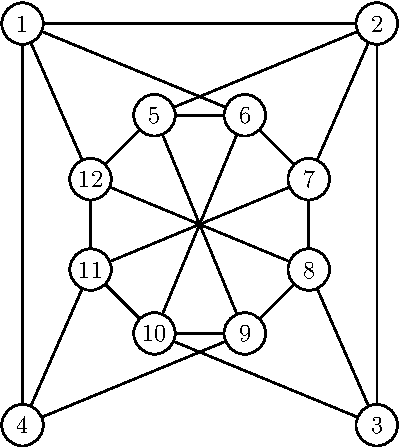
\includegraphics{graph-nocolor.pdf}
\caption{The graph $\mathcal{G}(V, E)$.\label{fig-graph-nocolor}}\end{figure}

The question, if $\mathcal{G}$ is $3$--colorable or not, is easy to answer by trial and error. We
are, however, an interested in algorithmic solution to the problem, so lets first encode $V$ and
$E$ of the graph $\mathcal{G}$ using Python's built--in data structures:

\begin{Verbatim}[commandchars=@\[\]]
@PYG[g+gp][@textgreater[]@textgreater[]@textgreater[] ]@PYG[n][V] @PYG[o][=] @PYG[n+nb][range]@PYG[p][(]@PYG[l+m+mi][1]@PYG[p][,] @PYG[l+m+mi][12]@PYG[o][+]@PYG[l+m+mi][1]@PYG[p][)]
@PYG[g+gp][@textgreater[]@textgreater[]@textgreater[] ]@PYG[n][E] @PYG[o][=] @PYG[p][@PYGZlb[]]@PYG[p][(]@PYG[l+m+mi][1]@PYG[p][,]@PYG[l+m+mi][2]@PYG[p][)]@PYG[p][,]@PYG[p][(]@PYG[l+m+mi][2]@PYG[p][,]@PYG[l+m+mi][3]@PYG[p][)]@PYG[p][,]@PYG[p][(]@PYG[l+m+mi][1]@PYG[p][,]@PYG[l+m+mi][4]@PYG[p][)]@PYG[p][,]@PYG[p][(]@PYG[l+m+mi][1]@PYG[p][,]@PYG[l+m+mi][6]@PYG[p][)]@PYG[p][,]@PYG[p][(]@PYG[l+m+mi][1]@PYG[p][,]@PYG[l+m+mi][12]@PYG[p][)]@PYG[p][,]@PYG[p][(]@PYG[l+m+mi][2]@PYG[p][,]@PYG[l+m+mi][5]@PYG[p][)]@PYG[p][,]@PYG[p][(]@PYG[l+m+mi][2]@PYG[p][,]@PYG[l+m+mi][7]@PYG[p][)]@PYG[p][,]@PYG[p][(]@PYG[l+m+mi][3]@PYG[p][,]@PYG[l+m+mi][8]@PYG[p][)]@PYG[p][,]
@PYG[g+gp][... ]@PYG[p][(]@PYG[l+m+mi][3]@PYG[p][,]@PYG[l+m+mi][10]@PYG[p][)]@PYG[p][,]@PYG[p][(]@PYG[l+m+mi][4]@PYG[p][,]@PYG[l+m+mi][11]@PYG[p][)]@PYG[p][,]@PYG[p][(]@PYG[l+m+mi][4]@PYG[p][,]@PYG[l+m+mi][9]@PYG[p][)]@PYG[p][,]@PYG[p][(]@PYG[l+m+mi][5]@PYG[p][,]@PYG[l+m+mi][6]@PYG[p][)]@PYG[p][,]@PYG[p][(]@PYG[l+m+mi][6]@PYG[p][,]@PYG[l+m+mi][7]@PYG[p][)]@PYG[p][,]@PYG[p][(]@PYG[l+m+mi][7]@PYG[p][,]@PYG[l+m+mi][8]@PYG[p][)]@PYG[p][,]@PYG[p][(]@PYG[l+m+mi][8]@PYG[p][,]@PYG[l+m+mi][9]@PYG[p][)]@PYG[p][,]@PYG[p][(]@PYG[l+m+mi][9]@PYG[p][,]@PYG[l+m+mi][10]@PYG[p][)]@PYG[p][,]
@PYG[g+gp][... ]@PYG[p][(]@PYG[l+m+mi][10]@PYG[p][,]@PYG[l+m+mi][11]@PYG[p][)]@PYG[p][,]@PYG[p][(]@PYG[l+m+mi][11]@PYG[p][,]@PYG[l+m+mi][12]@PYG[p][)]@PYG[p][,]@PYG[p][(]@PYG[l+m+mi][5]@PYG[p][,]@PYG[l+m+mi][12]@PYG[p][)]@PYG[p][,]@PYG[p][(]@PYG[l+m+mi][5]@PYG[p][,]@PYG[l+m+mi][9]@PYG[p][)]@PYG[p][,]@PYG[p][(]@PYG[l+m+mi][6]@PYG[p][,]@PYG[l+m+mi][10]@PYG[p][)]@PYG[p][,]@PYG[p][(]@PYG[l+m+mi][7]@PYG[p][,]@PYG[l+m+mi][11]@PYG[p][)]@PYG[p][,]@PYG[p][(]@PYG[l+m+mi][8]@PYG[p][,]@PYG[l+m+mi][12]@PYG[p][)]@PYG[p][@PYGZrb[]]
\end{Verbatim}
\noindent
We encoded the set of vertices as a list of consecutive integers and the set of edges as a list
of tuples of adjacent vertex indices. Next we will transform the graph into an algebraic form by
mapping vertices to variables and tuples of indices into tuples of variables:

\begin{Verbatim}[commandchars=@\[\]]
@PYG[g+gp][@textgreater[]@textgreater[]@textgreater[] ]@PYG[n][Vx] @PYG[o][=] @PYG[p][@PYGZlb[]] @PYG[n][Symbol]@PYG[p][(]@PYG[l+s][']@PYG[l+s][x]@PYG[l+s]['] @PYG[o][+] @PYG[n+nb][str]@PYG[p][(]@PYG[n][i]@PYG[p][)]@PYG[p][)] @PYG[k][for] @PYG[n][i] @PYG[o+ow][in] @PYG[n][V] @PYG[p][@PYGZrb[]]
@PYG[g+gp][@textgreater[]@textgreater[]@textgreater[] ]@PYG[n][Ex] @PYG[o][=] @PYG[p][@PYGZlb[]] @PYG[p][(]@PYG[n][Vx]@PYG[p][@PYGZlb[]]@PYG[n][i]@PYG[o][-]@PYG[l+m+mi][1]@PYG[p][@PYGZrb[]]@PYG[p][,] @PYG[n][Vx]@PYG[p][@PYGZlb[]]@PYG[n][j]@PYG[o][-]@PYG[l+m+mi][1]@PYG[p][@PYGZrb[]]@PYG[p][)] @PYG[k][for] @PYG[n][i]@PYG[p][,] @PYG[n][j] @PYG[o+ow][in] @PYG[n][E] @PYG[p][@PYGZrb[]]
\end{Verbatim}
\noindent
As the last step of this construction we write equations for $F_3$ and $F_{\mathcal{G}}$:

\begin{Verbatim}[commandchars=@\[\]]
@PYG[g+gp][@textgreater[]@textgreater[]@textgreater[] ]@PYG[n][F3] @PYG[o][=] @PYG[p][@PYGZlb[]] @PYG[n][x]@PYG[o][*]@PYG[o][*]@PYG[l+m+mi][3] @PYG[o][-] @PYG[l+m+mi][1] @PYG[k][for] @PYG[n][x] @PYG[o+ow][in] @PYG[n][Vx] @PYG[p][@PYGZrb[]]
@PYG[g+gp][@textgreater[]@textgreater[]@textgreater[] ]@PYG[n][Fg] @PYG[o][=] @PYG[p][@PYGZlb[]] @PYG[n][x]@PYG[o][*]@PYG[o][*]@PYG[l+m+mi][2] @PYG[o][+] @PYG[n][x]@PYG[o][*]@PYG[n][y] @PYG[o][+] @PYG[n][y]@PYG[o][*]@PYG[o][*]@PYG[l+m+mi][2] @PYG[k][for] @PYG[n][x]@PYG[p][,] @PYG[n][y] @PYG[o+ow][in] @PYG[n][Ex] @PYG[p][@PYGZrb[]]
\end{Verbatim}
\noindent
Everything is set following the theoretical introduction, so now we can compute the Gröbner
basis of $F_3 \cup F_{\mathcal{G}}$ with respect to \emph{lexicographic} ordering of terms:

\begin{Verbatim}[commandchars=@\[\]]
@PYG[g+gp][@textgreater[]@textgreater[]@textgreater[] ]@PYG[n][G] @PYG[o][=] @PYG[n][groebner]@PYG[p][(]@PYG[n][F3] @PYG[o][+] @PYG[n][Fg]@PYG[p][,] @PYG[n][Vx]@PYG[p][)]
\end{Verbatim}
\noindent
We know that if the constructed system of polynomial equations has a solution then $G$ should be
non--trivial, i.e. $G \not= \emptyset$, which can be easily verified in SymPy:

\begin{Verbatim}[commandchars=@\[\]]
@PYG[g+gp][@textgreater[]@textgreater[]@textgreater[] ]@PYG[n][G] @PYG[o][!=] @PYG[p][@PYGZlb[]]@PYG[l+m+mi][1]@PYG[p][@PYGZrb[]]
@PYG[g+go][True]
\end{Verbatim}
\noindent
The answer is that the graph $\mathcal{G}$ is colorable with $3$ colors. A sample coloring is shown
in figure \ref{fig-graph-color}. Suppose we add an edge between vertices $i = 3$ and $j = 4$. Is
the new graph $3$--colorable? To check this it is sufficient to construct $F_{\mathcal{G'}}$ by
extending $F_{\mathcal{G}}$ with $x_3^2 + x_3 x_4 + x_4^2$ equation and recompute the Gröbner
basis:

\begin{Verbatim}[commandchars=@\[\]]
@PYG[g+gp][@textgreater[]@textgreater[]@textgreater[] ]@PYG[n][x3]@PYG[p][,] @PYG[n][x4] @PYG[o][=] @PYG[n][Vx]@PYG[p][@PYGZlb[]]@PYG[l+m+mi][2]@PYG[p][@PYGZrb[]]@PYG[p][,] @PYG[n][Vx]@PYG[p][@PYGZlb[]]@PYG[l+m+mi][3]@PYG[p][@PYGZrb[]]

@PYG[g+gp][@textgreater[]@textgreater[]@textgreater[] ]@PYG[n][G] @PYG[o][=] @PYG[n][groebner]@PYG[p][(]@PYG[n][F3] @PYG[o][+] @PYG[n][Fg] @PYG[o][+] @PYG[p][@PYGZlb[]]@PYG[n][x3]@PYG[o][*]@PYG[o][*]@PYG[l+m+mi][2] @PYG[o][+] @PYG[n][x3]@PYG[o][*]@PYG[n][x4] @PYG[o][+] @PYG[n][x4]@PYG[o][*]@PYG[o][*]@PYG[l+m+mi][2]@PYG[p][@PYGZrb[]]@PYG[p][,] @PYG[n][Vx]@PYG[p][)]

@PYG[g+gp][@textgreater[]@textgreater[]@textgreater[] ]@PYG[n][G] @PYG[o][!=] @PYG[p][@PYGZlb[]]@PYG[l+m+mi][1]@PYG[p][@PYGZrb[]]
@PYG[g+go][False]
\end{Verbatim}
\noindent
We got a trivial Gröbner basis as the result, so the graph $\mathcal{G'}$ isn't $3$--colorable. We
could continue this discussion asking if $\mathcal{G'}$ is $4$--colorable or if the number of colors
required to color the original graph could be lowered to $2$ colors.
\begin{figure}[htbp]
\centering

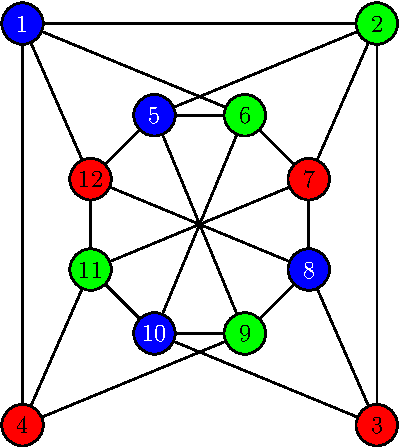
\includegraphics{graph-color.pdf}
\caption{A sample $3$--coloring of the graph $\mathcal{G}(V, E)$.\label{fig-graph-color}}\end{figure}

Before we compare SymPy`s syntax for computing Gröbner bases with other systems, let us clarify an
issue arising around list indexing (e.g. why we write \code{x3 = Vx{[}2{]}}). SymPy is a library built on top
of Python, so it utilizes Python's built--in data structures and their indexing schemes. Python, as a
general purpose programming language, uses well established zero--based indexing scheme, contrary to the
natural way of \emph{indexing} things, i.e. saying 1st, 2nd, 3rd etc. (to which we are accustomed in real life
and mathematics). The zero--based indexing scheme dates back to the time of first programming languages,
which were hardware oriented (e.g. assemblers) and an index was understood as an offset from a particular
location in memory (the start of a container) to the requested item (for a more detailed discussion about
this issue see \cite{Dijkstra1982zero}). General purpose programming languages, even those interpreted like
Python, coherently follow this scheme. For SymPy, this is a cost of building the system on top of a general
purpose language. As we will see in the following examples, other symbolic manipulation systems, i.e. those
which invent their own programming language, use \emph{natural indexing} scheme. Currently a workaround to have
one--based indexing in SymPy, is to append a dummy element in front of a list, e.g. to index \code{Vx} this
way we could issue \code{Vx = {[}None{]} + Vx} and then \code{x3 = Vx{[}3{]}}.


\subsubsection{Vertex coloring using other systems}

We showed so far how to solve classical vertex coloring problem with SymPy. Lets now compare SymPy`s
syntax and semantics of Gröbner bases functionality with three other mathematical software: Maxima,
Axiom and Mathematica.

One feature that makes SymPy different from other mathematical systems is that SymPy utilizes a general
purpose programming language for its core, modules and interaction with the user, whereas Maxima, Axiom
and Mathematica invent their own special languages for implementing their mathematical libraries and for
user interaction. This will require us to make some remarks also on the syntactic level.

Maxima, available at \href{http://maxima.sourceforge.net}{http://maxima.sourceforge.net}, implements Gröbner bases in an extension library.
Detailed documentation can be found in \cite{MaximaGroebner}. We will reuse the same example and, as much as
possible, the same computational approach. Maxima first requires us to load the Gröbner bases library.
Note that we write \code{grobner} in this case. User should also remember about putting a semicolon at the end
of every line. Next we define edges of the graph using a list of two element lists (there are no tuples in
Maxima).  Maxima uses very unusual syntax for variable assignment, utilizing colon for this purpose. In the
next step we define the list of variables \code{Vx} and systems of polynomial equations \code{F3} and \code{Fg}.
Instead of list comprehensions we use \code{makelist()} function. One should note that Maxima uses \code{\textasciicircum{}}
symbol for exponentiation, whereas Python uses this symbol for bitwise XOR operation. Finally we can compute
the Gröbner basis using \code{poly\_reduced\_grobner()}. Maxima by default assumes \emph{lexicographic} ordering
of monomials. This information can be changed only by setting a global variable. As the last step we
check if the computed basis is non--trivial, utilizing \code{is()} and \code{notequal()} functions. Lets
see full source code for this example:

\begin{Verbatim}[commandchars=@\[\]]
(i1) load(grobner);

(i2) E: @PYGZlb[]@PYGZlb[]1,2@PYGZrb[],@PYGZlb[]2,3@PYGZrb[],@PYGZlb[]1,4@PYGZrb[],@PYGZlb[]1,6@PYGZrb[],@PYGZlb[]1,12@PYGZrb[],@PYGZlb[]2,5@PYGZrb[],@PYGZlb[]2,7@PYGZrb[],@PYGZlb[]3,8@PYGZrb[],
@PYGZlb[]3,10@PYGZrb[],@PYGZlb[]4,11@PYGZrb[],@PYGZlb[]4,9@PYGZrb[],@PYGZlb[]5,6@PYGZrb[],@PYGZlb[]6,7@PYGZrb[],@PYGZlb[]7,8@PYGZrb[],@PYGZlb[]8,9@PYGZrb[],@PYGZlb[]9,10@PYGZrb[],@PYGZlb[]10,11@PYGZrb[],
@PYGZlb[]11,12@PYGZrb[],@PYGZlb[]5,12@PYGZrb[],@PYGZlb[]5,9@PYGZrb[],@PYGZlb[]6,10@PYGZrb[],@PYGZlb[]7,11@PYGZrb[],@PYGZlb[]8,12@PYGZrb[]@PYGZrb[];

(i3) Vx: makelist(concat("x", i), i, 1, 12);

(i4) F3: makelist(Vx@PYGZlb[]i@PYGZrb[]@textasciicircum[]3 - 1, i, 1, 12);
(i5) Fg: @PYGZlb[]@PYGZrb[];

(i6) for e in E do
        Fg: endcons(Vx@PYGZlb[]e@PYGZlb[]1@PYGZrb[]@PYGZrb[]@textasciicircum[]2 + Vx@PYGZlb[]e@PYGZlb[]1@PYGZrb[]@PYGZrb[]*Vx@PYGZlb[]e@PYGZlb[]2@PYGZrb[]@PYGZrb[] + Vx@PYGZlb[]e@PYGZlb[]2@PYGZrb[]@PYGZrb[]@textasciicircum[]2, Fg);

(i7) G: poly@_reduced@_grobner(append(F3, Fg), Vx);

(i8) is(notequal(G, @PYGZlb[]1@PYGZrb[]));
(o8) true
\end{Verbatim}
\noindent
Axiom, available at \href{http://axiom-developer.org}{http://axiom-developer.org}, implements Gröbner bases toolkit in its
core algebra library. The documentation on this matter, thought not very extensive, can be found in
\cite{Daly2003horizon}. Axiom uses a sophisticated autoloader of its library components, so explicit package
loading in not necessary.  As previously we start with the definition of the set of edges using a list of
list. On should notice that, this time, the assignment operator is \code{:=}. Semicolons at the end of lines
are not obligatory, however, useful for preventing printing of the results of computations. Next we define
\code{Vx} and \code{Ex} in a way very similar to Python, as Axiom supports list comprehensions. The main difference
is Axiom's approach to indexing lists. Axiom does not use an object oriented language, as one might presume
looking at the source code, and it doesn't support properties. This give opportunity for reusing the dot
operator for indexing purpose (notice also one--base indexes). Next definitions of \code{F3} and \code{Fg} are
almost equivalent to what we wrote using SymPy. Finally we compute the Gröbner basis using \code{groebner()}
function. Notice the \code{::} operator. It tells that the previously constructed polynomials should belong
to the domain that is on its right hand side, i.e. distributed multivariate polynomial in symbols from
\code{Vx} with coefficients over integers. At the end we check that the basis in non--trivial using \code{\textasciitilde{}=}
operator. Note that \code{\textasciitilde{}=} is not a comparison operator by default, but returns an unequality, so we
need to use coercion operator \code{@} to tell \code{\textasciitilde{}=} to end up with a \code{Boolean} result immediately.
Here is the full source code for this example:

\begin{Verbatim}[commandchars=@\[\]]
(1) -@textgreater[] E := @PYGZlb[]@PYGZlb[]1,2@PYGZrb[],@PYGZlb[]2,3@PYGZrb[],@PYGZlb[]1,4@PYGZrb[],@PYGZlb[]1,6@PYGZrb[],@PYGZlb[]1,12@PYGZrb[],@PYGZlb[]2,5@PYGZrb[],@PYGZlb[]2,7@PYGZrb[],
@PYGZlb[]3,8@PYGZrb[],@PYGZlb[]3,10@PYGZrb[],@PYGZlb[]4,11@PYGZrb[],@PYGZlb[]4,9@PYGZrb[],@PYGZlb[]5,6@PYGZrb[],@PYGZlb[]6,7@PYGZrb[],@PYGZlb[]7,8@PYGZrb[],@PYGZlb[]8,9@PYGZrb[],@PYGZlb[]9,10@PYGZrb[],
@PYGZlb[]10,11@PYGZrb[],@PYGZlb[]11,12@PYGZrb[],@PYGZlb[]5,12@PYGZrb[],@PYGZlb[]5,9@PYGZrb[],@PYGZlb[]6,10@PYGZrb[],@PYGZlb[]7,11@PYGZrb[],@PYGZlb[]8,12@PYGZrb[]@PYGZrb[];

(2) -@textgreater[] Vx := @PYGZlb[] concat("x", i::String)::Symbol for i in 1..12 @PYGZrb[];
(3) -@textgreater[] Ex := @PYGZlb[] @PYGZlb[]Vx.(e.1), Vx.(e.2)@PYGZrb[] for e in E @PYGZrb[];

(4) -@textgreater[] F3 := @PYGZlb[] x**3 - 1 for x in Vx @PYGZrb[];
(5) -@textgreater[] Fg := @PYGZlb[] e.1**2 + e.1*e.2 + e.2**2 for e in Ex@PYGZrb[];

(6) -@textgreater[] G := groebner(@PYGZlb[] f::DMP(Vx, INT) for f in concat(F3, Fg) @PYGZrb[]);

(7) -@textgreater[] (G @textasciitilde[]= @PYGZlb[]1@PYGZrb[]) @PYGZat[] Boolean
   (7) true
\end{Verbatim}
\noindent
Mathematica, available at \href{http://www.wolfram.com/mathematica/}{http://www.wolfram.com/mathematica/}, has extensive built--in support
for Gröbner bases. Detailed documentation on this matter can be found in \cite{MathematicaGroebner}.
Mathematica has a very peculiar language for interaction with the user and its syntax, which was
influence by the infix dialect of lisp (or m--lisp), is very different from other languages used
in symbolic mathematics, so will skip detailed syntactic comparison and refer the reader to
\cite{Wolfram2003book}.

\begin{Verbatim}[commandchars=@\[\]]
In@PYGZlb[]1@PYGZrb[]:= Unprotect@PYGZlb[]E@PYGZrb[];
In@PYGZlb[]2@PYGZrb[]:= E := {{1,2},{2,3},{1,4},{1,6},{1,12},{2,5},{2,7},
{3,8},{3,10},{4,11},{4,9},{5,6},{6,7},{7,8},{8,9},{9,10},
{10,11},{11,12},{5,12},{5,9},{6,10},{7,11},{8,12}}

In@PYGZlb[]3@PYGZrb[]:= Vx := Table@PYGZlb[]Symbol@PYGZlb[]"x" @textless[]@textgreater[] ToString@PYGZlb[]i@PYGZrb[]@PYGZrb[], {i,1,12}@PYGZrb[]
In@PYGZlb[]4@PYGZrb[]:= h@PYGZlb[]{i@_, j@_}@PYGZrb[] := Vx@PYGZlb[]@PYGZlb[]i@PYGZrb[]@PYGZrb[]@textasciicircum[]2 + Vx@PYGZlb[]@PYGZlb[]i@PYGZrb[]@PYGZrb[] Vx@PYGZlb[]@PYGZlb[]j@PYGZrb[]@PYGZrb[] + Vx@PYGZlb[]@PYGZlb[]j@PYGZrb[]@PYGZrb[]@textasciicircum[]2

In@PYGZlb[]5@PYGZrb[]:= F3 := Map@PYGZlb[](@#@textasciicircum[]3-1)@&, Vx@PYGZrb[]
In@PYGZlb[]6@PYGZrb[]:= Fg := Map@PYGZlb[]h, E@PYGZrb[]

In@PYGZlb[]7@PYGZrb[]:= G := GroebnerBasis@PYGZlb[]Join@PYGZlb[]F3, Fg@PYGZrb[], Vx@PYGZrb[]

In@PYGZlb[]8@PYGZrb[]:= G != {1}
Out@PYGZlb[]8@PYGZrb[]= True
\end{Verbatim}
\noindent
We showed how to perform classical vertex coloring of a graph based on the Gröbner bases method
using SymPy and three other mathematical systems. It is interesting to compare the times that were
needed to compute the Gröbner basis $G$ by each of those systems. Timings (average of multiple
runs) were collected in figure \ref{fig-groebner-time-compare}. This simple study shows that both
SymPy and Maxima are significantly slower than Axiom and Mathematica. This happens, because the
implementation of Gröbner bases in both systems is done in an interpreted language (Python and
Maxima language, respectively). Possibly they also implement less(--powerful) criteria for eliminating
useless critical pairs.
\begin{figure}[htbp]
\centering

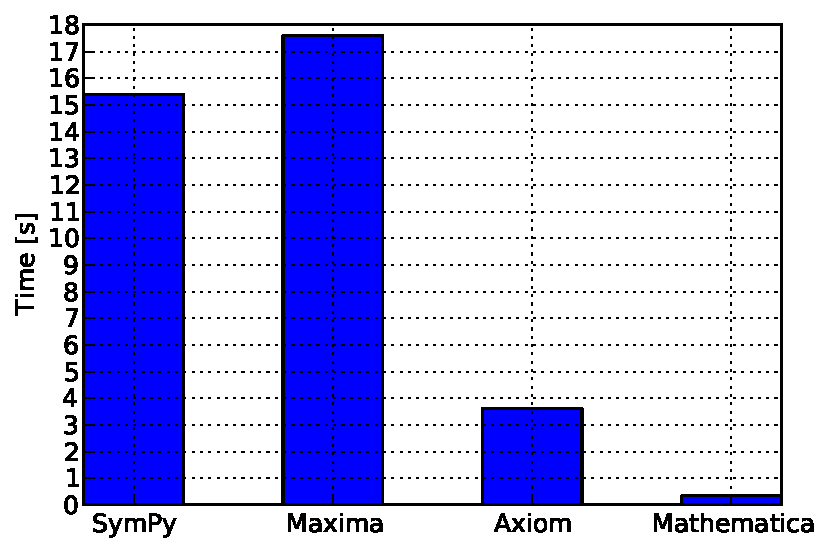
\includegraphics{groebner-time-compare.pdf}
\caption{Average timing for computing Gröbner basis of graph $\mathcal{G}(V, E)$.\label{fig-groebner-time-compare}}\end{figure}


\subsubsection{The structure of vertex coloring}

Till this point we showed how to check with SymPy that a graph is $k$--colorable or not. However, using
the Gröbner bases method, we can obtain a much more exciting result. Suppose that $G$ is a lexicographic
Gröbner basis of a system of polynomials $F$ describing a vertex $k$--coloring problem. To prove
that a graph is $k$--colorable we used the fact that $G \not= \{1\}$. We know that $G$ and $F$ have
the same set of solutions, however, $G$ has more structure than $F$. We can take advantage of this
and find all possible $k$--colorings of a graph by solving $G$ over the complex field.

Lets first revise our approach to vertex coloring. To transform a graph problem in a polynomial problem,
we mapped colors to primitive roots of unity. In our example of $3$--coloring, the three colors were, say
red, green and blue, were mapped to $1$, $\zeta$, $\zeta^2$, where $\zeta = \exp(\frac{2\pi\I}{k})$. In
other words we worked in a field generated by $\zeta$:

\begin{Verbatim}[commandchars=@\[\]]
@PYG[g+gp][@textgreater[]@textgreater[]@textgreater[] ]@PYG[n][zeta] @PYG[o][=] @PYG[n][exp]@PYG[p][(]@PYG[l+m+mi][2]@PYG[o][*]@PYG[n][pi]@PYG[o][*]@PYG[n][I]@PYG[o][/]@PYG[l+m+mi][3]@PYG[p][)]@PYG[o][.]@PYG[n][expand]@PYG[p][(]@PYG[n+nb][complex]@PYG[o][=]@PYG[n+nb+bp][True]@PYG[p][)]

@PYG[g+gp][@textgreater[]@textgreater[]@textgreater[] ]@PYG[n][zeta]
@PYG[g+go][    @_@_@_]
@PYG[g+go][I*@textbackslash[]/ 3]
@PYG[g+go][------- - 1/2]
@PYG[g+go][   2]
\end{Verbatim}
\noindent
Thus to tell that every vertex should be assigned a color we wrote a system of equations of the form
$x_i^3 - 1$, where $i \in \{1, \ldots, |V|\}$. Lets factor this polynomial over $\Q[\zeta]$:

\begin{Verbatim}[commandchars=@\[\]]
@PYG[g+gp][@textgreater[]@textgreater[]@textgreater[] ]@PYG[n][factor]@PYG[p][(]@PYG[n][x]@PYG[o][*]@PYG[o][*]@PYG[l+m+mi][3] @PYG[o][-] @PYG[l+m+mi][1]@PYG[p][,] @PYG[n][extension]@PYG[o][=]@PYG[n][zeta]@PYG[p][)]
@PYG[g+go][        /        @_@_@_      @textbackslash[] /        @_@_@_      @textbackslash[]]
@PYG[g+go][        |    I*@textbackslash[]/ 3       | |    I*@textbackslash[]/ 3       |]
@PYG[g+go][(x - 1)*|x + ------- + 1/2|*|x - ------- + 1/2|]
@PYG[g+go][        @textbackslash[]       2         / @textbackslash[]       2         /]
\end{Verbatim}
\noindent
We obtained the splitting factorization of $x_i^3 - 1$ and we can clearly see how our mapping works.
Lets now solve each of the above linear obtaining a list of primitive roots of unity of order three:

\begin{Verbatim}[commandchars=@\[\]]
@PYG[g+gp][@textgreater[]@textgreater[]@textgreater[] ]@PYG[p][@PYGZlb[]] @PYG[n][solve]@PYG[p][(]@PYG[n][arg]@PYG[p][)]@PYG[p][@PYGZlb[]]@PYG[l+m+mi][0]@PYG[p][@PYGZrb[]] @PYG[k][for] @PYG[n][arg] @PYG[o+ow][in] @PYG[n][@_]@PYG[o][.]@PYG[n][args] @PYG[p][@PYGZrb[]]
@PYG[g+go][[         @_@_@_            @_@_@_      ]]
@PYG[g+go][[     I*@textbackslash[]/ 3         I*@textbackslash[]/ 3       ]]
@PYG[g+go][[1, - ------- - 1/2, ------- - 1/2]]
@PYG[g+go][[        2              2         ]]
\end{Verbatim}
\noindent
Going one step ahead, lets declare three variables which will literally represent colors in the studied
$3$--coloring problem and lets put together, in an arbitrary but fixed order, those variables and the
previously computed roots of unity:

\begin{Verbatim}[commandchars=@\[\]]
@PYG[g+gp][@textgreater[]@textgreater[]@textgreater[] ]@PYG[n][var]@PYG[p][(]@PYG[l+s][']@PYG[l+s][red,green,blue]@PYG[l+s][']@PYG[p][)]
@PYG[g+go][(red, green, blue)]

@PYG[g+gp][@textgreater[]@textgreater[]@textgreater[] ]@PYG[n][colors] @PYG[o][=] @PYG[n+nb][zip]@PYG[p][(]@PYG[n][@_@_]@PYG[p][,] @PYG[n][@_]@PYG[p][)]

@PYG[g+gp][@textgreater[]@textgreater[]@textgreater[] ]@PYG[n][colors]
@PYG[g+go][[          /      @_@_@_             @textbackslash[]  /    @_@_@_            @textbackslash[]]]
@PYG[g+go][[          |  I*@textbackslash[]/ 3              |  |I*@textbackslash[]/ 3             |]]
@PYG[g+go][[(1, red), |- ------- - 1/2, green|, |------- - 1/2, blue|]]
@PYG[g+go][[          @textbackslash[]     2                /  @textbackslash[]   2               /]]
\end{Verbatim}
\noindent
Now we are prepared to study the structure of the Gröbner basis $G$. To make the analysis easier, we
we will split $G$ into groups, discriminating polynomials by their degree and their number of terms:

\begin{Verbatim}[commandchars=@\[\]]
@PYG[g+gp][@textgreater[]@textgreater[]@textgreater[] ]@PYG[n][key] @PYG[o][=] @PYG[k][lambda] @PYG[n][f]@PYG[p][:] @PYG[p][(]@PYG[n][degree]@PYG[p][(]@PYG[n][f]@PYG[p][)]@PYG[p][,] @PYG[n+nb][len]@PYG[p][(]@PYG[n][f]@PYG[o][.]@PYG[n][args]@PYG[p][)]@PYG[p][)]
@PYG[g+gp][@textgreater[]@textgreater[]@textgreater[] ]@PYG[n][groups] @PYG[o][=] @PYG[n][split]@PYG[p][(]@PYG[n][G]@PYG[p][,] @PYG[n][key]@PYG[p][,] @PYG[n][reverse]@PYG[o][=]@PYG[n+nb+bp][True]@PYG[p][)]

@PYG[g+gp][@textgreater[]@textgreater[]@textgreater[] ]@PYG[n+nb][len]@PYG[p][(]@PYG[n][groups]@PYG[p][)]
@PYG[g+go][4]
\end{Verbatim}
\noindent
We obtained four groups of polynomials, so lets analyzed them one--by--one:

\begin{Verbatim}[commandchars=@\[\]]
@PYG[g+gp][@textgreater[]@textgreater[]@textgreater[] ]@PYG[n][groups]@PYG[p][@PYGZlb[]]@PYG[l+m+mi][0]@PYG[p][@PYGZrb[]]
@PYG[g+go][[   3    ]]
@PYG[g+go][[x12  - 1]]
\end{Verbatim}
\noindent
In the first group we have just a single polynomial of the well known form. This tells us that $x_{12}$
can be assigned any of the three possible colors. This wasn't very interesting, so lets move the next
group:

\begin{Verbatim}[commandchars=@\[\]]
@PYG[g+gp][@textgreater[]@textgreater[]@textgreater[] ]@PYG[n][groups]@PYG[p][@PYGZlb[]]@PYG[l+m+mi][1]@PYG[p][@PYGZrb[]]
@PYG[g+go][[   2                2]]
@PYG[g+go][[x11  + x11*x12 + x12 ]]
\end{Verbatim}
\noindent
From the construction of the system of polynomials $F_{\mathcal{G}}$, which describes an admissible
vertex coloring for the graph $\mathcal{G}$, we know that the above equation is zero when $x_{11}$
is different from $x_{12}$. Still we didn't learn anything new, so lets move to the third group:

\begin{Verbatim}[commandchars=@\[\]]
@PYG[g+gp][@textgreater[]@textgreater[]@textgreater[] ]@PYG[n][groups]@PYG[p][@PYGZlb[]]@PYG[l+m+mi][2]@PYG[p][@PYGZrb[]]
@PYG[g+go][@PYGZlb[]x1 + x11 + x12, x11 + x12 + x5, x11 + x12 + x8, x10 + x11 + x12@PYGZrb[]]
\end{Verbatim}
\noindent
This time we got a lot more polynomials, which are of a new form. We should recall that we use
primitive roots of unity for color assignment. Roots of this kind have the property that their
sum is zero. So, from the above equations we can read that triples of vertices $x_i$, $x_{11}$
and $x_{12}$, where $i \in \{1, 5, 8, 10\}$, should be assigned different colors. This is a
piece of knowledge that we didn't see in $F$ but we were able to learn from $G$. Lets move
to the last group:

\begin{Verbatim}[commandchars=@\[\]]
@PYG[g+gp][@textgreater[]@textgreater[]@textgreater[] ]@PYG[n][groups]@PYG[p][@PYGZlb[]]@PYG[l+m+mi][3]@PYG[p][@PYGZrb[]]
@PYG[g+go][@PYGZlb[]-x11 + x2, -x12 + x3, -x12 + x4, -x11 + x6, -x12 + x7, -x11 + x9@PYGZrb[]]
\end{Verbatim}
\noindent
In the last group we got a set of trivial equations of the form $x_i = x_j$, which tell us that
particular pairs of vertices should have the same color assigned. What we described here is a
complete knowledge necessary to invent a $3$--coloring for $\mathcal{G}$.

Following this analysis of the structure of the Gröbner basis $G$, to find a $3$--coloring of
the graph $\mathcal{G}$, first we need to choose a color for $x_{12}$. Suppose we let $x_{12}$ to
have red color assigned. Then we have to assign a color other than red to $x_{11}$. Let it be green.
From the fourth group of equations from $G$ we know that $x_3$, $x_4$ and $x_7$ will be assigned the
same color as $x_{12}$, i.e. red, and $x_2$, $x_6$ and $x_9$ will have the same color as $x_{11}$,
i.e. blue. Then it is sufficient to assign other vertices, mainly $x_1$, $x_5$, $x_8$ and $x_{10}$,
with green color. This way we obtained a single admissible $3$--coloring of the graph $\mathcal{G}$
(the same as the coloring of figure \ref{fig-graph-color}).

What about other admissible $3$--colorings? We can continue with the above procedure and generate
more colorings. It would be, however, more interesting if we could get all solutions to our graph
problem at once. To do this with SymPy, we will simply solve $G$:

\begin{Verbatim}[commandchars=@\[\]]
@PYG[g+gp][@textgreater[]@textgreater[]@textgreater[] ]@PYG[n][colorings] @PYG[o][=] @PYG[n][solve]@PYG[p][(]@PYG[n][G]@PYG[p][,] @PYG[n][Vx]@PYG[p][)]

@PYG[g+gp][@textgreater[]@textgreater[]@textgreater[] ]@PYG[n+nb][len]@PYG[p][(]@PYG[n][colorings]@PYG[p][)]
@PYG[g+go][6]
\end{Verbatim}
\noindent
We got six admissible $3$--colorings for $\mathcal{G}$. This is correct because there are three ways
to assign $x_{12}$ a color, then there are only two ways to assign $x_{11}$ a color for each possible
coloring of $x_{12}$, and, with colors assigned to $x_{11}$ and $x_{12}$, there is only one way to
assign colors to other vertices.

At this point we could simply print the computed solutions to see what are the admissible $3$--colorings.
This is, however, not a good idea, because we use algebraic numbers (roots of unity) for representing colors
and \code{solve()} returned solutions in terms of those algebraic number, possibly even in a non--simplified
form. To overcome this difficulty we will use previously defined mapping between roots of unity and literal
colors:

\begin{Verbatim}[commandchars=@\[\]]
@PYG[g+gp][@textgreater[]@textgreater[]@textgreater[] ]@PYG[k][for] @PYG[n][coloring] @PYG[o+ow][in] @PYG[n][colorings]@PYG[p][:]
@PYG[g+gp][... ]    @PYG[k][print] @PYG[p][@PYGZlb[]] @PYG[n][elt]@PYG[o][.]@PYG[n][expand]@PYG[p][(]@PYG[n+nb][complex]@PYG[o][=]@PYG[n+nb+bp][True]@PYG[p][)]@PYG[o][.]@PYG[n][subs]@PYG[p][(]@PYG[n][colors]@PYG[p][)] @PYG[k][for] @PYG[n][elt] @PYG[o+ow][in] @PYG[n][coloring] @PYG[p][@PYGZrb[]]
@PYG[g+gp][...]
@PYG[g+gp][...]
@PYG[g+go][@PYGZlb[]blue, green, red, red, blue, green, red, blue, green, blue, green, red@PYGZrb[]]
@PYG[g+go][@PYGZlb[]green, blue, red, red, green, blue, red, green, blue, green, blue, red@PYGZrb[]]
@PYG[g+go][@PYGZlb[]green, red, blue, blue, green, red, blue, green, red, green, red, blue@PYGZrb[]]
@PYG[g+go][@PYGZlb[]red, green, blue, blue, red, green, blue, red, green, red, green, blue@PYGZrb[]]
@PYG[g+go][@PYGZlb[]blue, red, green, green, blue, red, green, blue, red, blue, red, green@PYGZrb[]]
@PYG[g+go][@PYGZlb[]red, blue, green, green, red, blue, green, red, blue, red, blue, green@PYGZrb[]]
\end{Verbatim}
\noindent
This is the result we were looking for, but a few words of explanation are needed. As \code{solve()} may
return unsimplified results, we need to simplify any algebraic numbers that don't match structurally with
the precomputed roots of unity. Taking advantage of the domain of computation, we use complex expansion
algorithm for this purpose. Having the solutions in a normal form, to get this nice form with literal
colors it is sufficient to substitute \emph{color} variables for roots of unity.

There is one more important thing, which we must emphasise. When solving the Gröbner basis $G$, we
specified the list of symbols explicitly using \code{Vx}. In general this is unnecessary and \code{solve()}
can work perfectly without this knowledge. However, in our case this additional piece of information
was significant, because it guaranteed proper order of color assignments in the solution. Most functions
in SymPy can derive variables of the problem being solved on their own, but in complex situations this
may lead to wrong results or at least can complicate analysis of solutions. If unsure what a particular
function will do, always specify variables explicitly.


\subsection{Algebraic geometry}

Geometry is one of the primary subjects taught during elementary mathematics classes and using SymPy for
studying theorems of Euclidean geometry seems a very promising idea. For example, lets consider a rhombus
(in a fixed coordinate system). We would like to prove a theorem that diagonals of a rhombus are mutually
perpendicular. We are of course interested in a purely algorithmic approach to solve this problem. To prove
this theorem we will use the machinery of Gröbner bases.

Following \cite{Winkler1990geometry}, lets consider a geometric entity which properties can be translated into a
system of $m$ polynomials, say $\mathcal{H} = \{f_1, \ldots, f_m\}$. We will call $\mathcal{H}$ a hypothesis.
Given a theorem concerning this geometric entity, the algebraic formulation is as follows:
\begin{gather}
\begin{split}\forall_{x_1, \ldots, x_n, y_1, \ldots, y_n} (f_1 = 0 \vee \ldots \vee f_m = 0) \Rightarrow g = 0\end{split}\notag
\end{gather}
where $g$ is the conclusion of the theorem and $f_1, \ldots f_m$ and $g$ are polynomials in $\K[x_1, \ldots,
x_n, y_1, \ldots, y_n]$. It follows from the Gröbner bases theory that the above statement is true when $g$
belongs to the ideal generated by $\mathcal{H}$. To check this, i.e. to prove the theorem, it is sufficient
to compute Gröbner basis of $\mathcal{H}$ and reduce $g$ with respect to this basis. If the theorem is
true then the remainder from the reduction will vanish. In this example, for the sake of simplicity, we
assume that the geometric entity is non--degenerate, i.e. it does not collapse into a line or a point.
Anyway, the Gröbner basis approach allows to prove theorems in algebraic geometry in full generality
and derive automatically non--degeneracy conditions.
\begin{figure}[htbp]
\centering

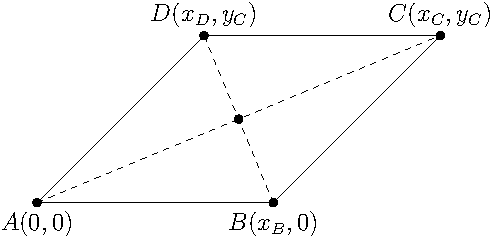
\includegraphics{geometry-rhombus.pdf}
\caption{A rhombus in a fixed coordinate system.\label{fig-geometry-rhombus}}\end{figure}

Lets consider the rhombus of figure \ref{fig-geometry-rhombus}. This geometric entity consists of four
points $A$, $B$, $C$ and $D$. To setup a fixed coordinate system, without loss of generality, we can
assume that $A = (0, 0)$, $B = (x_B, 0)$, $C = (x_C, y_C)$ and $D = (x_D, y_D)$. This is possible by
taking rotational invariance of the geometric entity. We will prove that the diagonals of this rhombus,
i.e. $AD$ and $BC$ are mutually perpendicular. We have the following conditions describing $ABCD$:
\begin{enumerate}
\item {} 
Line $AD$ is parallel to $BC$, i.e. $AD \parallel BC$.

\item {} 
Sides of $ABCD$ are of the equal length, i.e. $AB = BC$.

\item {} 
The rhombus is non--degenerate, i.e. is not a line or a point.

\end{enumerate}

Our conclusion is that $AC \bot BD$. To prove this theorem, first we need to transform the above conditions
and the conclusion into a set of polynomials. How we can achieve this? Lets focus on the first condition. In
general, we are given two lines $A_1A_2$ and $B_1B_2$. To express the relation between those two lines, i.e.
that $A_1A_2$ is parallel $B_1B_2$, we can relate slopes of those lines:
\begin{gather}
\begin{split}\frac{y_{A_2} - y_{A_1}}{x_{A_2} - x_{A_1}} = \frac{y_{B_2} - y_{B_1}}{x_{B_2} - x_{B_1}}\end{split}\notag
\end{gather}
Clearing denominators in the above expression and putting all terms on the left hand side of the equation, we
derive a general polynomial describing the first condition. This can be literally translated into Python:

\begin{Verbatim}[commandchars=@\[\]]
@PYG[k][def] @PYG[n+nf][parallel]@PYG[p][(]@PYG[n][A1]@PYG[p][,] @PYG[n][A2]@PYG[p][,] @PYG[n][B1]@PYG[p][,] @PYG[n][B2]@PYG[p][)]@PYG[p][:]
    @PYG[l+s+sd]["""Line @PYGZlb[]A1, A2@PYGZrb[] is parallel to line @PYGZlb[]B1, B2@PYGZrb[]. """]
    @PYG[k][return] @PYG[p][(]@PYG[n][A2]@PYG[o][.]@PYG[n][y] @PYG[o][-] @PYG[n][A1]@PYG[o][.]@PYG[n][y]@PYG[p][)]@PYG[o][*]@PYG[p][(]@PYG[n][B2]@PYG[o][.]@PYG[n][x] @PYG[o][-] @PYG[n][B1]@PYG[o][.]@PYG[n][x]@PYG[p][)] @PYG[o][-] @PYG[p][(]@PYG[n][B2]@PYG[o][.]@PYG[n][y] @PYG[o][-] @PYG[n][B1]@PYG[o][.]@PYG[n][y]@PYG[p][)]@PYG[o][*]@PYG[p][(]@PYG[n][A2]@PYG[o][.]@PYG[n][x] @PYG[o][-] @PYG[n][A1]@PYG[o][.]@PYG[n][x]@PYG[p][)]
\end{Verbatim}
\noindent
assuming that \code{A1}, \code{A2}, \code{B1} and \code{B2} are instances of \code{Point} class. In the case of our
rhombus, we will take advantage of the fixed coordinate system and simplify the resulting polynomials as
much as possible. The same approach can be used to derive polynomial representation for other conditions
and the conclusion. To construct $\mathcal{H}$ and $g$ we will use the following functions:

\begin{Verbatim}[commandchars=@\[\]]
@PYG[k][def] @PYG[n+nf][distance]@PYG[p][(]@PYG[n][A1]@PYG[p][,] @PYG[n][A2]@PYG[p][)]@PYG[p][:]
    @PYG[l+s+sd]["""The squared distance between points A1 and A2. """]
    @PYG[k][return] @PYG[p][(]@PYG[n][A2]@PYG[o][.]@PYG[n][x] @PYG[o][-] @PYG[n][A1]@PYG[o][.]@PYG[n][x]@PYG[p][)]@PYG[o][*]@PYG[o][*]@PYG[l+m+mi][2] @PYG[o][+] @PYG[p][(]@PYG[n][A2]@PYG[o][.]@PYG[n][y] @PYG[o][-] @PYG[n][A1]@PYG[o][.]@PYG[n][y]@PYG[p][)]@PYG[o][*]@PYG[o][*]@PYG[l+m+mi][2]

@PYG[k][def] @PYG[n+nf][equal]@PYG[p][(]@PYG[n][A1]@PYG[p][,] @PYG[n][A2]@PYG[p][,] @PYG[n][B1]@PYG[p][,] @PYG[n][B2]@PYG[p][)]@PYG[p][:]
    @PYG[l+s+sd]["""Lines @PYGZlb[]A1, A2@PYGZrb[] and @PYGZlb[]B1, B2@PYGZrb[] are of the same width. """]
    @PYG[k][return] @PYG[n][distance]@PYG[p][(]@PYG[n][A1]@PYG[p][,] @PYG[n][A2]@PYG[p][)] @PYG[o][-] @PYG[n][distance]@PYG[p][(]@PYG[n][B1]@PYG[p][,] @PYG[n][B2]@PYG[p][)]

@PYG[k][def] @PYG[n+nf][perpendicular]@PYG[p][(]@PYG[n][A1]@PYG[p][,] @PYG[n][A2]@PYG[p][,] @PYG[n][B1]@PYG[p][,] @PYG[n][B2]@PYG[p][)]@PYG[p][:]
    @PYG[l+s+sd]["""Line @PYGZlb[]A1, A2@PYGZrb[] is perpendicular to line @PYGZlb[]B1, B2@PYGZrb[]. """]
    @PYG[k][return] @PYG[p][(]@PYG[n][A2]@PYG[o][.]@PYG[n][x] @PYG[o][-] @PYG[n][A1]@PYG[o][.]@PYG[n][x]@PYG[p][)]@PYG[o][*]@PYG[p][(]@PYG[n][B2]@PYG[o][.]@PYG[n][x] @PYG[o][-] @PYG[n][B1]@PYG[o][.]@PYG[n][x]@PYG[p][)] @PYG[o][+] @PYG[p][(]@PYG[n][A2]@PYG[o][.]@PYG[n][y] @PYG[o][-] @PYG[n][A1]@PYG[o][.]@PYG[n][y]@PYG[p][)]@PYG[o][*]@PYG[p][(]@PYG[n][B2]@PYG[o][.]@PYG[n][y] @PYG[o][-] @PYG[n][B1]@PYG[o][.]@PYG[n][y]@PYG[p][)]
\end{Verbatim}
\noindent
The non--degeneracy statement requires a few words of comment. Many theorems in geometry are true only
in the non--degenerative case and false or undefined otherwise. In our approach to theorem proving in
algebraic geometry, we must supply sufficient non--degeneracy conditions manually. In the case of our
rhombus this is $x_B > 0$ and $y_C > 0$ (we don't need to take $x_C$ into account because $AB = BC$).
At first, this seems to be a show stopper, as Gröbner bases don't support inequalities. However,
we can use Rabinovich trick and transform those inequalities into a single polynomial condition by
introducing an additional variable, say $a$, about which we will assume that is positive. This gives
us a non--degeneracy condition $x_B y_C - a$.

With all this knowledge we are ready to prove the main theorem. First, lets declare variables:

\begin{Verbatim}[commandchars=@\[\]]
@PYG[g+gp][@textgreater[]@textgreater[]@textgreater[] ]@PYG[n][var]@PYG[p][(]@PYG[l+s][']@PYG[l+s][x@_B, x@_C, y@_C, x@_D, a]@PYG[l+s][']@PYG[p][)]
@PYG[g+go][(x@_B, x@_C, y@_C, x@_D, a)]

@PYG[g+gp][@textgreater[]@textgreater[]@textgreater[] ]@PYG[n+nb][vars] @PYG[o][=] @PYG[n][@_]@PYG[p][@PYGZlb[]]@PYG[p][:]@PYG[o][-]@PYG[l+m+mi][1]@PYG[p][@PYGZrb[]]
\end{Verbatim}
\noindent
We had to declare the additional variable $a$, but we don't consider it a variable of our problem. This
will lead to a new case in SymPy`s implementation of Gröbner bases, because we will be computing not
over rationals, as we did in all previous examples, but the computations will be done over the field of
univariate rational functions. Lets now define the four points $A$, $B$, $C$ and $D$:

\begin{Verbatim}[commandchars=@\[\]]
@PYG[g+gp][@textgreater[]@textgreater[]@textgreater[] ]@PYG[n][A] @PYG[o][=] @PYG[n][Point]@PYG[p][(]@PYG[l+m+mi][0]@PYG[p][,] @PYG[l+m+mi][0]@PYG[p][)]
@PYG[g+gp][@textgreater[]@textgreater[]@textgreater[] ]@PYG[n][B] @PYG[o][=] @PYG[n][Point]@PYG[p][(]@PYG[n][x@_B]@PYG[p][,] @PYG[l+m+mi][0]@PYG[p][)]
@PYG[g+gp][@textgreater[]@textgreater[]@textgreater[] ]@PYG[n][C] @PYG[o][=] @PYG[n][Point]@PYG[p][(]@PYG[n][x@_C]@PYG[p][,] @PYG[n][y@_C]@PYG[p][)]
@PYG[g+gp][@textgreater[]@textgreater[]@textgreater[] ]@PYG[n][D] @PYG[o][=] @PYG[n][Point]@PYG[p][(]@PYG[n][x@_D]@PYG[p][,] @PYG[n][y@_C]@PYG[p][)]
\end{Verbatim}
\noindent
Using the previously defined functions we can define the hypothesis:

\begin{Verbatim}[commandchars=@\[\]]
@PYG[g+gp][@textgreater[]@textgreater[]@textgreater[] ]@PYG[n][h1] @PYG[o][=] @PYG[n][parallel]@PYG[p][(]@PYG[n][A]@PYG[p][,] @PYG[n][D]@PYG[p][,] @PYG[n][B]@PYG[p][,] @PYG[n][C]@PYG[p][)]
@PYG[g+gp][@textgreater[]@textgreater[]@textgreater[] ]@PYG[n][h2] @PYG[o][=] @PYG[n][equal]@PYG[p][(]@PYG[n][A]@PYG[p][,] @PYG[n][B]@PYG[p][,] @PYG[n][B]@PYG[p][,] @PYG[n][C]@PYG[p][)]
@PYG[g+gp][@textgreater[]@textgreater[]@textgreater[] ]@PYG[n][h3] @PYG[o][=] @PYG[n][x@_B]@PYG[o][*]@PYG[n][y@_C] @PYG[o][-] @PYG[n][a]
\end{Verbatim}
\noindent
and compute its Gröbner basis:

\begin{Verbatim}[commandchars=@\[\]]
@PYG[g+gp][@textgreater[]@textgreater[]@textgreater[] ]@PYG[n][G] @PYG[o][=] @PYG[n][groebner]@PYG[p][(]@PYG[p][@PYGZlb[]]@PYG[n][h1]@PYG[p][,] @PYG[n][h2]@PYG[p][,] @PYG[n][h3]@PYG[p][@PYGZrb[]]@PYG[p][,] @PYG[n+nb][vars]@PYG[p][,] @PYG[n][order]@PYG[o][=]@PYG[l+s][']@PYG[l+s][grlex]@PYG[l+s][']@PYG[p][)]
\end{Verbatim}
\noindent
Two things need a comment here. Previously we specified variables in \code{groebner()}, when we were
concerned about the order of variables. This was necessary when the task was to eliminate particular
variables, before proceeding to the other steps of an algorithm. However, in this case we are rather
concerned about not letting the variable $a$ to be considered as a significant variable in the problem,
because we treat $a$ as a parameter. The other thing is that we can compute the Gröbner basis with
respect to any admissible ordering of monomials. We chose the standard total degree scheme, over the
default lexicographic ordering, because leads to shorter computation times.

Lets now verify the theorem:

\begin{Verbatim}[commandchars=@\[\]]
@PYG[g+gp][@textgreater[]@textgreater[]@textgreater[] ]@PYG[n][reduced]@PYG[p][(]@PYG[n][perpendicular]@PYG[p][(]@PYG[n][A]@PYG[p][,] @PYG[n][C]@PYG[p][,] @PYG[n][B]@PYG[p][,] @PYG[n][D]@PYG[p][)]@PYG[p][,] @PYG[n][G]@PYG[p][,] @PYG[n+nb][vars]@PYG[p][,] @PYG[n][order]@PYG[o][=]@PYG[l+s][']@PYG[l+s][grlex]@PYG[l+s][']@PYG[p][)]@PYG[p][@PYGZlb[]]@PYG[l+m+mi][1]@PYG[p][@PYGZrb[]]
@PYG[g+go][0]
\end{Verbatim}
\noindent
This proves that $AC \bot BD$. Although, the theorem we described and proved was a simple one, one can
handle much more complicated problems as well. One should refer to Winkler's paper for more interesting
examples, especially concerning issues with degenerate cases.


\subsection{Other applications}

So far several detailed examples of practical applications of the Gröbner bases method were
presented, which explained most interesting features of Gröbner bases and their use patterns
in SymPy. Following the list from the beginning of this section, there are, however, many more
applications. We will give reference to several of them in this part.

Besides the obvious application of solving systems of polynomial equations and the less obvious
for computing LCMs and GCDs of multivariate polynomials, the Gröbner basis method is also used
in SymPy for computing minimal polynomials of algebraic numbers, primitive elements of algebraic
fields and isomorphisms between algebraic fields (for a detailed theoretical discussion see
\cite{Adams1994intro} and algorithms refer to \cite{Cohen1993course}). For all those tasks there
are much more efficient algorithms implemented in SymPy. However, Gröbner bases remain the
fallback tool if any of the fast algorithms isn't suitable for a particular job. For example,
minimal polynomials can be relatively easily computed using PSLQ algorithm (see \code{pslq()}
function in mpmath library) but only in the case of real algebraic numbers. In the more general
case of complex algebraic numbers the Gröbner bases method is the only choice.

Gröbner bases can be also directly applicable in symbolic manipulation systems for computing
factorizations of multivariate polynomials \cite{Gianni1985groebner} or evaluating symbolic summations
and integrals \cite{Chyzak1998groebner}.


\section{Complexity of computing Gröbner bases}

Depending on our point of view, the complexity of the Gröbner bases method may vary. Gröbner
bases can be considered easy when we are discussing the general idea that stands behind them, or
the structure of Buchberger algorithm. As we saw in section \ref{gb-construct}, the operations
needed to compute a Gröbner basis are elementary and taught in high--school, and it shouldn't be
very difficult, for a high--school student, to experiment with Gröbner bases, especially in Python.

However, the algorithmic complexity of the Gröbner basis method is very high. This is not a
surprise, as in the examples we were able to solve several problems which intrinsic complexity
is exponential. Thus, in the general setup, the Buchberger has exponential complexity as well,
whereas in \emph{pathological} cases its complexity may increase to doubly exponential. It should be
emphasised that the Buchberger algorithm is very fragile to the choice of the ordering of
monomials, so it often happens that a Gröbner basis, for a set of polynomials, with respect
to one ordering is computable in relatively short time, whereas to compute it with respect to
another ordering one would have to wait ages. Lexicographic Gröbner bases are considered to
be the most expensive ones. In \cite{Buchberger2001systems} we can find a simple--looking system
of three polynomials in three variables:
\begin{gather}
\begin{split}\left\{
\begin{array}{l}
    x y^3 - 2 y z - z^2 + 13          \\
    y^2 - x^2 z + x z^2 + 3           \\
    z^2 x - y^2 x^2 + x y + y^3 + 12
\end{array}
\right.\end{split}\notag
\end{gather}
for which a Gröbner basis with respect to lexicographic ordering can't be computed in a \emph{reasonable}
time in SymPy. However, if we switch to graded lexicographic ordering of monomials, SymPy requires
less than a second to construct the basis. For comparison, Mathematica can compute both bases at glance
(refer to \cite{MathematicaInternal} for a description of its implementation of Buchberger algorithm).

However, as the examples showed us, there is often a lot of \emph{structure} in the Gröbner bases found
in practical applications, so many non--trivial and interesting Gröbner bases are relatively simple
to compute.

There many improvements possible to the SymPy`s implementation of Buchberger algorithm. Techniques like
Gröbner Walk, which allows to compute a basis with respect to a \emph{cheaper} ordering of monomials first
and then convert it to a more expensive one, or linear algebra approach \cite{Faugere1999f4}, in which a
polynomial algebra problem is transformed in into a linear algebra problem and solved using efficient
algorithms available in this field, are all applicable in SymPy. Ideas for improving the Gröbner
bases module are listed, among other, as \emph{Google Summer of Code} proposals at \cite{SymPyGSoC2010}.

Currently the most promising approach for improving the Buchberger algorithm is SymPy, which is scheduled
for implementation in near future, is algorithm F5 due to Jean Charles Faugère (see \cite{Faugere2002f5} and
\cite{Stegers2006f5}). The algorithm has the same structure as Buchberger algorithm, however it utilizes a very
powerful criteria for elimination of useless critical pairs, significantly reducing the number of required
polynomial divisions.  In practical cases there are \emph{no} reductions to zero in F5 algorithm. Reductions to
zero may happen in certain situations, however, their number is still less than in any other algorithm for
computing Gröbner bases. Thus F5 is considered to be at least one order of magnitude faster than the
fastest algorithm previously available.


\section{Conclusions}

The Gröbner bases method is a powerful tool in symbolic and algebraic computing, which is currently
not yet fully utilized in SymPy. Also implementation of Buchberger's algorithm is quite limited at
the moment. However, as we showed in this chapter, SymPy can be used for solving practical problems
in symbolic mathematics, specifically problems which involve solving systems of polynomials. We hope
that, in foreseeable future, improved algorithms for computing Gröbner bases will be implemented,
so that SymPy will be able to tackle more complex problems.



\chapter{Final words and conclusions}\label{thesis-conclusions}

In this thesis the author summed up three years of his work on computer algebra module for
SymPy, a library for symbolic mathematics in pure Python. We showed the state of art in
symbolic and algebraic computing, and described SymPy and its goals as a side effect. We
also introduced polynomials manipulation module, which was the central part of this thesis.
In three chapters we described the internal design and algorithms of the module, and showed
some practical examples of its applications. Not everything could have be written in this
volume, due to its limited capacity, however, the author hopes that this text have given
at least basic insight into what symbolic and algebraic computing in pure Python is. Time
and users' interest (or not) in SymPy and its polynomials manipulation module, will show
if it was the right decision to design and implement such software from scratch, in an
interpreted, dynamically typed programming language. In the remainder of this chapter we
will briefly describe the future of the module and possible further developments.


\section{Future plans}

After three years of development and, especially, after such an important milestone as master's
thesis is, a question arises: is this the end? Or, if this is not an end, how much work is still
in front of us? In this thesis we already often speculated about future developments that could,
or better should, be done to improve polynomials manipulation module. In the field of symbolic
and algebraic computing, tree years are not enough to catch up with other software that is on
the market for 20, 30 or even 40 years. We hope that SymPy and its computer algebra module
will steadily grow and more cutting edge algorithms will be implemented in it. To point out
some of the future ways in which the module might be heading, we devote the rest of this section
to list some ideas for future development. This is obviously and more ideas can be found in
the source code, documentation and SymPy`s web pages, especially those concerning Google
Summer of Code program.


\subsection{Polynomial arithmetics}

We already said quite a lot about arithmetics of polynomials, also about possible improvements
in this area. Improvements that are commonly known the many people, not necessarily interested
very much in computer algebra. However, there are other, less familiar algorithms for doing
polynomial arithmetics, especially of large sparse multivariate polynomials, which are not
limited to integer or rational domains. A nice example are algorithms for polynomial multiplication
and division based on heaps \cite{Monagan2007heaps}. Experimental data reveals that this is currently
the best approach to compute with sparse polynomials in many variables (which is actually the
most important case when computing with polynomials). The algorithm can also be relatively
easily parallelized, see \cite{Monagan2009parallel} for detailed discussion.


\subsection{Power series expansion}

SymPy implements a very modern algorithm of Gruntz for computing limits symbolically \cite{Gruntz1996limits},
thus, as a side effect, SymPy is quite comprehensible in computing truncated power series of elementary
and special functions (Taylor and Laurent series). When the algorithms for those two tasks were implemented,
polynomials manipulation module was almost non--existent, so everything was implemented using slow symbolic
core. This makes any computations concerning limits and power series very slow, because the underlying
algorithms are implemented in an inefficient way. Many benchmarks show that SymPy can be enormously slow
when computing series expansions of composite functions or when many terms are requested.

It would be beneficial to improve this picture by employing efficient polynomials manipulation algorithms
whenever possible, when computing limits and power series. Additional algorithms would have to be added
to the module, to allow efficient compositions and reversions of power series \cite{Zippel1976expansions},
\cite{Brent1975series}, \cite{Brent1978fps}. This would be very advantageous for SymPy, because limits and
truncated power series are ubiquitous in other algorithms of symbolic mathematics and are also very
useful as standalone tools in many practical problems.


\subsection{Partial fraction decomposition}

Decomposition algorithms of rational functions into partial fractions are also very useful tools
in symbolic mathematics. In SymPy we currently implement an algorithm of Manuel Bronstein
\cite{Bronstein1993partial}, which allows to compute full partial fraction decompositions purely
formally, without introducing algebraic numbers. This is a spectacular approach, but also a
quite inefficient one. It would be beneficial to incorporate modular techniques into partial
fraction decomposition algorithms, for example using methods of \cite{Wang1981partial}. This would
allow computations of partial fractions efficiently whenever possible and Bronstein's algorithm
would be used as a fallback.


\subsection{Simplification of expressions}

Polynomial manipulation algorithms have a natural area of application, which is simplification
of expressions \cite{Moses1971simplification}. Currently we already employ algorithms related to
polynomials for this task, but we do not utilize their full potential in this case. Expression
simplification is ubiquitous in symbolic mathematics systems, thus it must be general on hand but
also very efficient on the other. One very interesting case is simplification of rational functions
with polynomial side relations (modulo polynomial ideals), which was already studied in detail in
literature \cite{Pearce2001relations}, \cite{Monagan2006modulo}. This kind of simplification would allow
the user to compute efficiently with expressions like trigonometric polynomials, which are an
important tool in geometry and robotics.


\subsection{Cylindrical algebraic decomposition}

Currently one of big weaknesses of polynomials manipulation module is lack of solvers for multivariate
polynomial inequalities and systems of polynomial inequalities. SymPy can solve many kinds of problems
related to polynomial equations and systems of polynomial equations, thanks to the Gröbner bases
method. It can also handle univariate inequalities via root isolation. However, multivariate inequalities,
especially over reals, are currently a no--go for SymPy. The real case is very important, because it is
related to the problem of quantifier elimination and theorem proving in algebraic geometry.

A tool that is needed to allow SymPy for handling multivariate inequalities is cylindrical algebraic
decomposition \cite{Arnon1984basic}, \cite{Jirstrand1995cylindrical}, or CAD for short. Given a multivariate
polynomial inequality or system of inequalities, CAD decomposes those inequalities to form a system
of inequalities that are easier to reason about. This has many applications in, already mentioned,
quantifier elimination and algebraic geometry, but also when evaluating multiple integrals and in
assumptions engine.


\subsection{Multiple algebraic extensions}

In section \ref{thesis-algebraic} we said that SymPy currently requires to compute a primitive
element of a field extension if multiple extensions are provided, when computing with algebraic
numbers. We also gave references to articles concerning polynomial factoring algorithms, which
can work directly with multiple extensions. There are, however, algorithms for other areas of
symbolic mathematics, for example for computing GCDs of polynomials \cite{vanHoeij2002modgcd}, that
also do not require primitive element computations. Although, it is uncertain if those algorithms
are truly advantageous, it might be still worthwhile to experiment with them.


\subsection{Using modular techniques elsewhere}

Work on polynomials manipulation module revealed that, so called, modular or p--adic techniques
\cite{Yun1976padic}, give very encouraging results when concerned about speed of computations. Many
classes of algorithms already benefit from this in SymPy, most notable are factorization and
resultant algorithms, and other, like polynomial GCD algorithms, will be in future implemented.

Following this success, we should incorporate modular techniques outside polynomials manipulation
module. We already pointed out a method for computing partial fraction decomposition, but there
are other areas where those methods are applicable. A good examples are algorithms for symbolic
summation and integration \cite{Gerhard2006modular}. Modular method limit the range of application
of algorithms to integers and rationals, but those are the most commonly used domains in SymPy,
so the hassle is definitely worthwhile.

